%!TEX TS-program = lualatex
% dissertation.tex -- main dissertation file
%
% Wisconsin dissertation template
% Copyright (c) 2008-2009 William C. Benton.  All rights reserved.
%
% This program can redistributed and/or modified under the terms
% of the LaTeX Project Public License Distributed from CTAN
% archives in directory macros/latex/base/lppl.txt; either
% version 1 of the License, or (at your option) any later version.
%
% This program includes other software that is licensed under the
% terms of the LPPL and the Perl Artistic License; see README for details.
%
% You, the user, still hold the copyright to any document you produce
% with this software (like your dissertation).
%

\DocumentMetadata{
    lang = en-US,
    pdfversion = 2.0,
    pdfstandard = ua-2,
    tagging = on,
    tagging-setup = {math/setup=mathml-SE},
    testphase = {phase-III, math, table, firstaid} 
}

%%% You'll want ``oneside'' for the deposit version, but probably not for any versions that don't need to meet the UW requirements
\documentclass[12pt,oneside,letterpaper]{report}

% preamble.tex -- packages to include
%
% Wisconsin dissertation template
% Copyright (c) 2008 William C. Benton.  All rights reserved.
%
% This program can redistributed and/or modified under the terms
% of the LaTeX Project Public License Distributed from CTAN
% archives in directory macros/latex/base/lppl.txt; either
% version 1 of the License, or (at your option) any later version.
%
% This program includes other software that is licensed under the
% terms of the LPPL and the Perl Artistic License; see README for details.
%
% You, the user, still hold the copyright to any document you produce
% with this software (like your dissertation).

%% You should use natbib
\IfFileExists{natbib.sty}{%
\usepackage[authoryear,round]{natbib}%
}{}

%% You probably need appendix, if you want appendices
\IfFileExists{appendix.sty}{%
\usepackage{appendix}%
}{}

% Page Setup
\usepackage[width=156mm,top=35mm,bottom=25.4mm,bindingoffset=0mm]{geometry}
\usepackage{fancyhdr}
\usepackage{setspace}
\pagestyle{fancyplain}
\fancyhf{}
\fancyhead[R]{\thepage}
\renewcommand{\headrulewidth}{0pt}
\setlength{\headheight}{15pt}

%% the spacing in memoir is weird, you'll need to use this
% \DisemulatePackage{setspace}
% \usepackage[onehalfspacing]{setspace}

\IfFileExists{enumitem.sty}{%
\usepackage[loadonly]{enumitem}[2007/06/30]%
\newlist{hanglist}{enumerate}{1}%
\setlist[hanglist]{label=\arabic*.}%
\setlist[hanglist,1]{leftmargin=0pt}%
}{%
\newenvironment{hanglist}{\begin{enumerate}}{\end{enumerate}}%
}

% For Feynman Diagrams
\usepackage{tikz}
\usepackage[compat=1.1.0]{tikz-feynman}

% For Feynman Diagrams
\usepackage{tikz}
\usepackage[compat=1.1.0]{tikz-feynman}

\usepackage{bookmark}
\makeatletter
\patchcmd{\@chapter}{%
  \m@mpn@new@chaptrue%
}{%
  \m@mpn@new@chaptrue%
  \ifdef\ch@pt@c{}{\def\ch@pt@c{}}%
}{}{\PackageWarning{dissertation}{Could not patch \protect\@chapter (ch@pt@c init)}}
\patchcmd{\@chapter}{%
  \def\f@rtoc{#2}%
  \def\f@rhdr{#2}%
}{%
  \gdef\f@rtoc{#2}%
  \gdef\f@rhdr{#2}%
}{}{\PackageWarning{dissertation}{Could not patch \protect\@chapter (branch 1)}}
\patchcmd{\@chapter}{%
  \let\f@rtoc\ch@pt@c
}{%
  \global\let\f@rtoc\ch@pt@c
}{}{\PackageWarning{dissertation}{Could not patch \protect\@chapter (branch 2)}}
\makeatother

\usepackage{todonotes}
\usepackage{subcaption}
\usepackage{url}

\IfFileExists{mathpartir.sty}{%
\usepackage{mathpartir}%
}{}

\IfFileExists{listings.sty}{%
\usepackage{listings}%
}{}

\hypersetup{pdfborder = 0 0 0}

\IfFileExists{microtype.sty}{%
\usepackage[protrusion=true,expansion=true]{microtype}%
}{}

\usepackage{boxedminipage}

\IfFileExists{booktabs.sty}{%
\usepackage{booktabs}%
}{}

\usepackage{ifpdf}

\usepackage{lmodern}
\usepackage[T1]{fontenc}

\IfFileExists{tgpagella.sty}{%
\usepackage{tgpagella}%
}{}

\usepackage{eulervm}

\usepackage{imakeidx}
\makeindex

\makeatletter
\newenvironment{wb-bib}[1]{%
  \chapter*{references}
\ifnobibintoc\else
\phantomsection
\addcontentsline{toc}{chapter}{References}
\fi
\prebibhook
  \begin{bibitemlist}{#1}}{\end{bibitemlist}\postbibhook}

\setcitestyle{square}
\newcommand{\prd}{Physical Review D}

\usepackage{tagpdf}
\tagpdfsetup{
  activate-all,
  math/alt/use,
  interwordspace=true,
}

\usepackage{tabularx}
\usepackage{siunitx}
\usepackage{array}
\usepackage{booktabs}
\newcolumntype{Y}{>{\centering\arraybackslash}X}

\usepackage{hyperref}
\hypersetup{
  pdftitle={Search for Neutrinos with Energy Greater than 10^16 eV Using All 5 Stations of the Askaryan Radio Array at the South Pole},
  pdfauthor={Abigail Bishop},
  pdfkeywords={Neutrino, Ultra-high energy, Askaryan, Radio},
  colorlinks=true,
  linkcolor=blue,
  urlcolor=blue,
  citecolor=black,
  pdfdisplaydoctitle=true,
}
\newcounter{Hfootnote}

\usepackage{unicode-math}
\setmathfont{Latin Modern Math} 

\newcommand{\arasim}{\texttt{AraSim}}
\newcommand{\araroot}{\texttt{AraRoot}}
\newcommand{\nuleptonsim}{\texttt{NuLeptonSim}}
\input{includes/defs}
\input{includes/thesisdefs}
\svnidlong{$LastChangedBy$}{$LastChangedRevision$}{$LastChangedDate$}{$HeadURL: http://freevariable.com/dissertation/branches/diss-template/dissertation.tex $} 

\begin{document}

\pagecolor{white}

% \clearpage
\pagenumbering{roman}  % This makes the page numbers Roman (i, ii, etc)

\makeatletter
\gdef\@title{Search for Neutrinos with Energy Greater than $\boldsymbol{10^{16}}$~eV Using All 5 Stations of the Askaryan Radio Array at the South Pole}
\gdef\@author{Abigail Rae Huffaker Bishop}
\gdef\@department{(Physics)}
\gdef\@date{2026}
\makeatother

%%% Uncomment the following if your .bib contains references that you will not 
%%% explicitly cite, but that should be in the final bibliography:
% \nocite{*}

\ifpdf
\DeclareGraphicsExtensions{.pdf, .jpg, .tif}
\else
\DeclareGraphicsExtensions{.eps, .jpg}
\fi

\maketitle

%% Add \part declarations if you want, but it's not necessary
%\part{Preliminaries}

\svnidlong{$LastChangedBy$}{$LastChangedRevision$}{$LastChangedDate$}{$HeadURL: http://freevariable.com/dissertation/branches/diss-template/frontmatter/frontmatter.tex $}
\vcinfo{}

%%% SOME OF THIS CODE IS ADAPTED FROM THE VENERABLE withesis.cls

% COPYRIGHT PAGE
%  - To include a copyright page use \copyrightpage
\copyrightpage

% DEDICATION
\begin{dedication}
	\emph{for all who accompanied me on this journey}
\end{dedication}


% ACKNOWLEDGMENTS
\begin{acks}
% \comment{Introduction, it takes a village.}

% I am very grateful to my advisor, Albrecht Karle, for his support in the many, different eras of my graduate school career. 
% Thank you for entrusting me to complete my work in Madison, Florida, Brussels, and at the South Pole. 
% I am so appreciative that every time I told you of scientific interest of mine, you connected me with avenues to explore them.
% Thank you for all the help with this thesis over the past few weeks and for everything over the past 6 years. 

% I would also like to thank my committee members, Keith Bechtol, Snežana Stanimirović, and Brian Clark, for extending their time and energy to helping me cross this finish line.

% I owe many thanks to the colleagues I collaborated with during my graduate career. 
% I am very grateful to Askaryan Radio Array (ARA) leadership for trusting me to redeploy our stations at the South Pole and to Radio Neutrino Observatory Greenland leadership for naming me as a backup for field deployment two years in a row.
% The operations and maintenance of the ARA discussed in Chapter~\ref{chap:ARA} would not be possible without the support of John Kelley, Cosmin Deaconu, Brian Clark. 
% The Operations Leads during my tenure included Jorge Torres, Alisa Nozdrina, Justin Flaherty, Alan Salcedo Gomez, Alex Machtay, and Shoukat Ali. 
% We also extend our utmost thanks to the support of the IceCube Maintenance and Operations team and Winter Overs for their support of ARA.
% We also thank the Wisconsin IceCube Particle Astrophysics Center for supporting ARA data and computation, namely Jim Bellinger, Patrick Meade, Steve Barnet, and David Schultz. 
% The simulation team I worked with which enabled the work of Chapter~\ref{chap:veff}, Appendix~\ref{app:AraSim}, and the simulations used in Chapter~\ref{chap:5sa_cleaning} and Chapter~\ref{chap:5sa_analysis} includes Alan Salcedo Gomez, Marco Muzio, Ryan Krebs, Austin Cummings, Brian Clark, and Will Luszczak.
% The analysis of ARA data presented in Chapter~\ref{chap:5sa_cleaning} and Chapter~\ref{chap:5sa_analysis} was completed by a team led by Marco Muzio and composed of myself, Alan Salcedo Gomez, Brian Clark, Mohammad Ful Hossain Seikh, Pawan Giri, and Alex Machtay. 
% Alan and I took over the analysis of A2 and A3 from Myoungchul Kim who's meticulous documentation we still consult years later.
% These simulation and analysis teams have been my primary associates over the past 4 years and I am so proud of what we have accomplished together.
% To Alan and Marco, I am especially thankful for our rapport of cheering each other up, helping each other through endless AraSim bugs, and standing by each other's sides.
% The initial CAD design for the antenna centralizers discussed in Appendix~\ref{app:spacers} was created by Jeff Cherwinka before I took over development with Albrecht Karle.
% Lastly, the study of event reconstruction using radio antennas in the IceCube-Gen2 Optical volume presented in Appendix~\ref{chap:gen2_infill} was completed with Lu Lu, Albrecht Karle, and Ben Hokanson-Fasig.

% I am grateful to countless colleagues who have supported me and believed in me on this journey. 
% At WIPAC this includes Ben, Kayla, Laura, Thomas, Ali, Luca, Zach, Hannah, Delaney, and Jessie who taught me more than I can express.
% My fellow graduate students Cameron, Sophia, Jack, Sassella, Jill, Rob, Juan, Trevor helped lighten any dark mood that was thrown our way.
% At the VUB and ULB, I have Simona, Nick, Dieder, Felix, Yarno, Simon DK, Jethro, Simon C, Quique, and Mitja to thank for many great lunches, random treats, and conversations about our field.
% I am also grateful to the Belgian American Education Foundation for the grant which supported my work in Belgium.
% I'd also like to thank Mike Zingale and Tom Shiland, previous mentors of mine who I have leaned on for support and encouragement throughout my academic journey. 
% And Steven Cotts, whose Calculus Cuisinart and electric lessons ignited my love for physics in the first place. 

% I lastly have many friends and family who deserve more thanks than I could possibly give.
% My dear friends Marie, Patrik, Sarah M, Lucie, Castro, and Jessie who have been by my side through thick and through thin.
% Skyler, Mackenzie, Mindi, and Bryan for cheering me on for as long as I can remember. 
% My brother, for loving my cat for me while I was travelling.
% My Papa, Uncle Bubble, Aunt Linda, and Uncle Darrel for all their encouragement and support.
% My Mama, for always being eager to hear me practice a talk or proofread an application statement for me. 
% And my best friend Sarah, for her boundless support, understanding, and kindness. 
% I'm thankful for the many, many years we have spent growing with each other and can't wait to see where we go next.
% I wouldn't be the person I am today if it weren't for her.
% Lastly, the real reason I got up every morning, was Melody, Leia, Ellie, and Rosie.
% I would not have made it through without their love and joy.
\end{acks}

% CONTENTS, TABLES, FIGURES

% \captionnamefont{\small\sffamily} 
% \captiontitlefont{\small\sffamily} 

% \renewcommand{\contentsname}{contents}
% \renewcommand{\listfigurename}{list of figures}
% \renewcommand{\listtablename}{list of tables}

\tableofcontents

\clearpage
\listoftables

\clearpage
\listoffigures

\clearpage
% NOMENCLATURE
% \begin{conventions}
% % \begin{description}
% % \item{\makebox[0.75in][l]{term}
% %        \parbox[t]{5in}{definition\\}}
% % \end{description}
% \input{conventions}
% \end{conventions}

%% The UW graduate school no longer wants a UMI abstract page
%% Should you need one for some reason, uncomment the following
%% lines.  Thanks to Matt Fredrikson for reporting this!

% \advisorname{Gottlob Frege}
% \advisortitle{Professor}
% \begin{umiabstract}
%  \svnidlong{$LastChangedBy$}{$LastChangedRevision$}{$LastChangedDate$}{$HeadURL: http://freevariable.com/dissertation/branches/diss-template/frontmatter/abstract.tex $}
\vcinfo{}

Ultra-high energy (UHE, $E>100$~PeV) neutrinos are a rare piece of multi-messenger astrophysics and are especially valuable for understanding the UHE cosmic ray flux and composition. 
When UHE neutrinos interact in dielectric media, they initiate particle cascades that emit optical-wavelength Cherenkov and radio-wavelength Askaryan emission.
The highest energy neutrino ever detected had an energy of $\sim220$~PeV and was found by KM3NeT via Cherenkov Radiation in the Mediterranean Sea emitted by the $\sim120$~PeV muon created in the parent neutrino's interaction~\citep{km3net_neutrino}. 
The IceCube Neutrino Observatory has also observed multiple neutrinos with energies over 1~PeV via Cherekov Radiation in the Antarctic Ice Sheet at the South Pole~\citep{icecube_ehe}.
Monitoring ice for Askaryan Radiation is also promising due to long attenuation and scattering lengths for radio emission in ice, allowing a single detector to observe UHE neutrino interactions many kilometers away. 
Radio-based UHE neutrino detectors have observed Askaryan emission in ice from cosmic ray showers \citep{ara_cr, arianna_cr, anita_cr} but no radio-based detector has observed a neutrino candidate yet. 

This thesis comprises simulations and analyses dedicated to finding UHE neutrinos using in-ice detectors at the South Pole and Greenland. 
Chapter~\ref{chap:intro} introduction to the field of UHE neutrino observations and it's place in multi-messenger astrophysics. 
A simulation study is then presented in Chapter~\ref{chap:gen2_infill} quantifying the benefits of joint Askaryan and Cherenkov emission observations in the proposed expansion of the IceCube Neutrino Observatory by placing radio antennas above all planned optical modules. 
Next, Chapter~\ref{chap:ARA} describes the Askaryan Radio Array (ARA) and a literature review of previous results from the ARA collaboration is presented.
The following Chapter~\ref{chap:veff} details simulation studies of ARA's sensitivity to UHE neutrinos, featuring the simulation of outgoing particles so that events like KM3NeT's UHE neutrino are considered in ARA's performance and characterized for potential observations. 
Chapter~\ref{chap:5sa_cleaning} and Chapter~\ref{chap:5sa_analysis} of this thesis describe the data cleaning and analysis of ARA's second station in the context of an array-wide, decadal neutrino search over the full array.
The thesis then concludes with Chapter~\ref{chap:conclusion} summarizing all discussed topics and presenting next steps and suggestions for future detectors and UHE neutrino analyses, especially in the context of the Radio Neutrino Observatory of Greenland and IceCube-Gen2 Radio \citep{rnog_design, icecube_gen2}. 

\comment{Can I share the antenna centering spacers somewhere in here?}
% \end{umiabstract}

\begin{abstract}
  \svnidlong{$LastChangedBy$}{$LastChangedRevision$}{$LastChangedDate$}{$HeadURL: http://freevariable.com/dissertation/branches/diss-template/frontmatter/abstract.tex $}
\vcinfo{}

Ultra-high energy (UHE, $E>100$~PeV) neutrinos are a rare piece of multi-messenger astrophysics and are especially valuable for understanding the UHE cosmic ray flux and composition. 
When UHE neutrinos interact in dielectric media, they initiate particle cascades that emit optical-wavelength Cherenkov and radio-wavelength Askaryan emission.
The highest energy neutrino ever detected had an energy of $\sim220$~PeV and was found by KM3NeT via Cherenkov Radiation in the Mediterranean Sea emitted by the $\sim120$~PeV muon created in the parent neutrino's interaction~\citep{km3net_neutrino}. 
The IceCube Neutrino Observatory has also observed multiple neutrinos with energies over 1~PeV via Cherekov Radiation in the Antarctic Ice Sheet at the South Pole~\citep{icecube_ehe}.
Monitoring ice for Askaryan Radiation is also promising due to long attenuation and scattering lengths for radio emission in ice, allowing a single detector to observe UHE neutrino interactions many kilometers away. 
Radio-based UHE neutrino detectors have observed Askaryan emission in ice from cosmic ray showers \citep{ara_cr, arianna_cr, anita_cr} but no radio-based detector has observed a neutrino candidate yet. 

This thesis comprises simulations and analyses dedicated to finding UHE neutrinos using in-ice detectors at the South Pole and Greenland. 
Chapter~\ref{chap:intro} introduction to the field of UHE neutrino observations and it's place in multi-messenger astrophysics. 
A simulation study is then presented in Chapter~\ref{chap:gen2_infill} quantifying the benefits of joint Askaryan and Cherenkov emission observations in the proposed expansion of the IceCube Neutrino Observatory by placing radio antennas above all planned optical modules. 
Next, Chapter~\ref{chap:ARA} describes the Askaryan Radio Array (ARA) and a literature review of previous results from the ARA collaboration is presented.
The following Chapter~\ref{chap:veff} details simulation studies of ARA's sensitivity to UHE neutrinos, featuring the simulation of outgoing particles so that events like KM3NeT's UHE neutrino are considered in ARA's performance and characterized for potential observations. 
Chapter~\ref{chap:5sa_cleaning} and Chapter~\ref{chap:5sa_analysis} of this thesis describe the data cleaning and analysis of ARA's second station in the context of an array-wide, decadal neutrino search over the full array.
The thesis then concludes with Chapter~\ref{chap:conclusion} summarizing all discussed topics and presenting next steps and suggestions for future detectors and UHE neutrino analyses, especially in the context of the Radio Neutrino Observatory of Greenland and IceCube-Gen2 Radio \citep{rnog_design, icecube_gen2}. 

\comment{Can I share the antenna centering spacers somewhere in here?} 
\end{abstract}

\clearpage\pagenumbering{arabic}

%%% END STUFF TAKEN FROM WITHESIS EXAMPLE FILE


%% Now include the tex files for each chapter, like so (I put these in separate dirs): 
\doublespacing 
% \include{intro/intro}
% \include{motivation/motivation}
% \include{related/related}
\chapter{Data Cleaning for the Five Station Analysis}

  The data taken by the Askaryan Radio Array have been analyzed a few times for neutrinos, solar flares, and to deduce the properties of the ice at the South Pole. 
  When the livetime of the five stations is added together, there are roughly 28 station-years of data but only 9 years of that data have been analyzed.
  This is partly because each station takes so long to calibrate and prepare for analysis but also because there is so much data to clean before one can perform an analysis. 
  For example, 8 of the station years that have been analyzed were analyzed by a team lead by two graduate students. 
  ARA currently has 5 graduate students, 2 postdoctoral researchers, and a faculty member who are devoted to analyzing the full 28 station-years of ARA data. 
  This process involves building an analysis pipeline from the ground up, cleaning years of data, and simulating neutrino and noise events then viewing how many are removed through the cleaning pipeline, and analyzing remaining events for neutrino signals. 
  
\section{Simulation Setup for Data Cleaning}

  It is important to consider how each cut translates to overall data loss and expected neutrino event data loss. 
  Neutrino events are therefore simulated uniformly in log( energy ) space with energies from $10^{15}$ eV to $10^{21}$ eV. 
  As in Chapter 4 Section 4, neutrinos are thrown in a forward simulation along trajectories that intersect with a cylinder 15~km in radius and 3~km in depth. % Fix this reference, use variables
  These neutrinos interact randomly within the Earth and all outgoing particles with energy greater than $10^{16}$ eV are simulated further. 
  Muon and tau stochastic losses, tau decays, and outgoing neutrino interactions are simulated. 
  
  Noise simulations are also generated using the spectral coefficients calculated from the "software trigger" events that are read out once per second, regardless of sufficient signal to trigger the detector. % Check the frequency of these events
  \missingfigure{Noise spectral coefficients for A2}
  \missingfigure{Example of a software trigger event and a simulated noise event.}
  
  The traces of the signal simulations and noise simulations are fed through the cleaning pipeline so that, as cuts are applied to remove backgrounds from the dataset, we can ensure that we are doing so in a way that maximized the potential residual neutrino event population. 
  At the end of data cleaning, the goal is that our data distributions for key analysis variables resemble the noise simulation distributions such that any outliers that may arise are due to neutrino events. 
  
\section{Defining Livetime Configurations for A2 \label{sec:a2configs}}

  The behavior of detector triggering and readout changes dramatically as the detector's configuration is changed. 
  This has serious effects on event reconstruction and analysis, so each station's livetime is divided into livetime configurations. 
  These livetime configurations are mostly based on antenna/string masking, trigger window, and the amount of waveform readout ahead of the bin that triggered the detector, called the pre-trigger readout window or the number of pre-RF blocks. 
  Each trigger block is 10~ns and the total trigger window is defined as 
  \begin{equation}
    TW = (N_{TB}+1) * 10~\text(ns)
    \ref{eq:trigwin}
  \end{equation}
  and the default trigger window is 10 blocks meaning 110~ns.
  Each RF block is 20~ns and the default setting for pre-RF blocks is 10, so the default pre-trigger readout window is 200~ns. 
  As a station needs three like-polarization antennas to trigger, there may be signal recorded one or more antennas in advance of the bin that triggered so it's important to tune the number of pre-RF blocks accordingly. 
  Having too few pre-RF blocks yielded poor reconstruction of calibration pulser events in configuration 6 of station 2 after String 1 was masked and was noticed in June 2020 on an Operations Call and adjusted. 
  \missingfigure{Examples of Calpulser events in A2C5, C6, and C7}
  \missingfigure{Reconstructed calpulser vs unixtime to show deterioration in C6}
  
  Figure~\ref{fig:configs} shows the evolution of these key parameters for the full station 2 livetime along with shaded regions indicating each defined livetime configuration. 
  What is not pictured in this figure is the masking of String 1 of Station 2 which began on run 15527 in January of 2020. 
  Note that these configurations have changed since the 4 year survey of Stations 2 and 3. 
  That analysis placed emphasis on the masked antennas, trigger window, presence of trigger delays, and full readout window length. 
  This analysis has discovered that the latter 2 settings are less impactful when defining run configurations compared to the antenna masking, trigger window, and recently appreciated pre-trigger readout window. 
  Further considering each new livetime configuration requires a distinct set of noise, signal, and effective volume simulations that take well over a hundred thousand CPU-hours to generate, livetime configuration permutations are minimized by only considering the trigger window, pre-trigger readout window, and the status of antenna masking. 
  \missingfigure{trigger window and pre RF blocks over time for A2 \label{fig:configs}}
  \missingfigure{Table of the configs like the one on the Wiki}
  
\section{Using the AraProc Analysis Pipeline}

  AraProc is a python-based framework spearheaded by Dr Marco Muzio and Professor Brian Clark that reads in L1 ARA data and converts it into condensed L2 data. % Provide the link
  The root-formatted L1 data include raw waveforms that take up roughly 7 GB of space per full run. 
  The root-formatted L2 data is created using the L1 data but only includes simple metadata and analysis variables describing each event, so full runs of L2 data only take up roughly 6 MB of space. 
  The preexisting metadata saved includes the time of an event, the trigger type, and the detector configuration among other settings. 
  The calculated analysis variables generated by AraProc include the reconstructed azimuth, zenith, and signal correlation for nearby "pulser" maps and distant 300m maps for each polarization (horizontal and vertical) as well as direct and refracted rays for the distant maps. 
  The radius of the pulser map used for the reconstruction is uniquely set to the physical distance from a station's pulser to the station's center.
  Other analysis variables include the SNR of the coherently summed waveform for an event, the average RMS of the waveforms, the impulsivity, and the spark power ratios. 
  Some of these analysis variables will be explained in more detail in the coming sections as they are used to employ various cuts. 
  The AraProc framework can be run on computing clusters so many runs may be processed in parallel. 
  \todo{Showcase some of the analysis variables}
  
\section{Removing Spoiled Data}

  The first genre of cuts that will be discussed are those that remove bad events from the data. 
  These events are usually the result of digitizing malfunctions. 
  
  \subsection{1st Minute Cut}
  
    During the first minute of a run, events from ARA stations are typically corrupted as the waveforms recorded usually have a large offset compared to the pedestal values of the waveform. 
    This is the result of unstable power draw in the station as it starts a new run. 
    Due to this large offset, it is expected that the average waveform RMS and SNR are abnormal during the first minute of a run compared to the remainder of the run. 
    Shown in Figure~\ref{fig:firstmin_waveform} are the waveforms in every ARA2 channel for an event in the first minute of a run. 
    Figure~\ref{fig:firstmin_2d} shows how the average waveform RMS changes in the first 10 minutes of a run as well. 
    The impulsive nature of these waveforms can mimic the neutrino signal this analysis is targeting so these events must be removed from the analysis. 
    
    
    \begin{figure}
      \centering
      \begin{subfigure}[t]{0.48\textwidth}
        \centering
        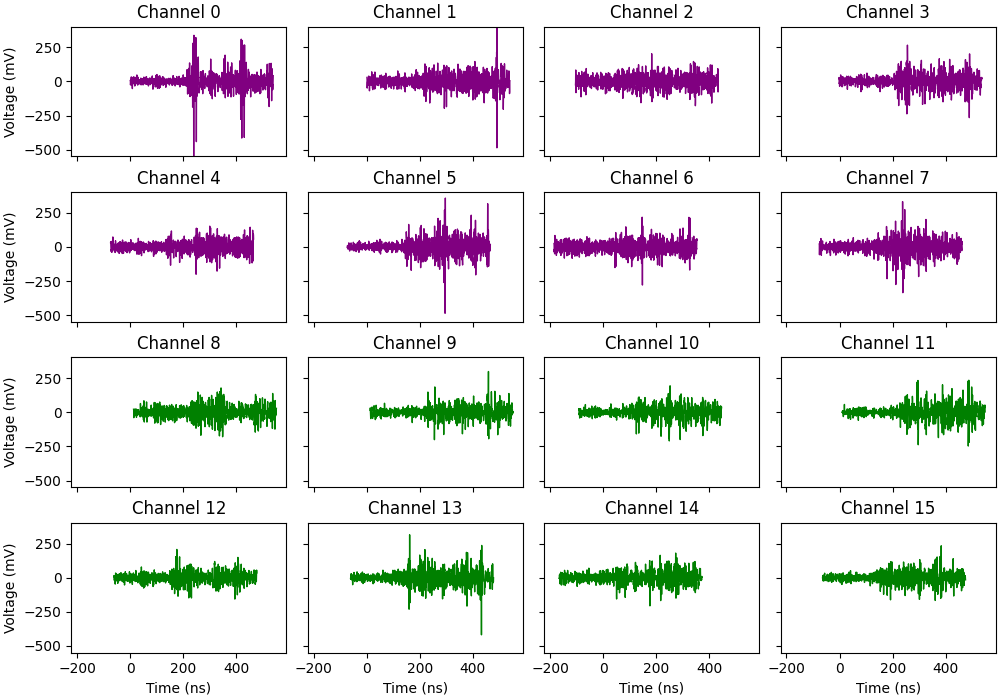
\includegraphics[width=\textwidth]{sections/5sa-cleaning/images/firstmin_station_2_run_17627_eventNo_2_trace.png}
      \end{subfigure}
      ~
      \begin{subfigure}[t]{0.48\textwidth}
        \centering
        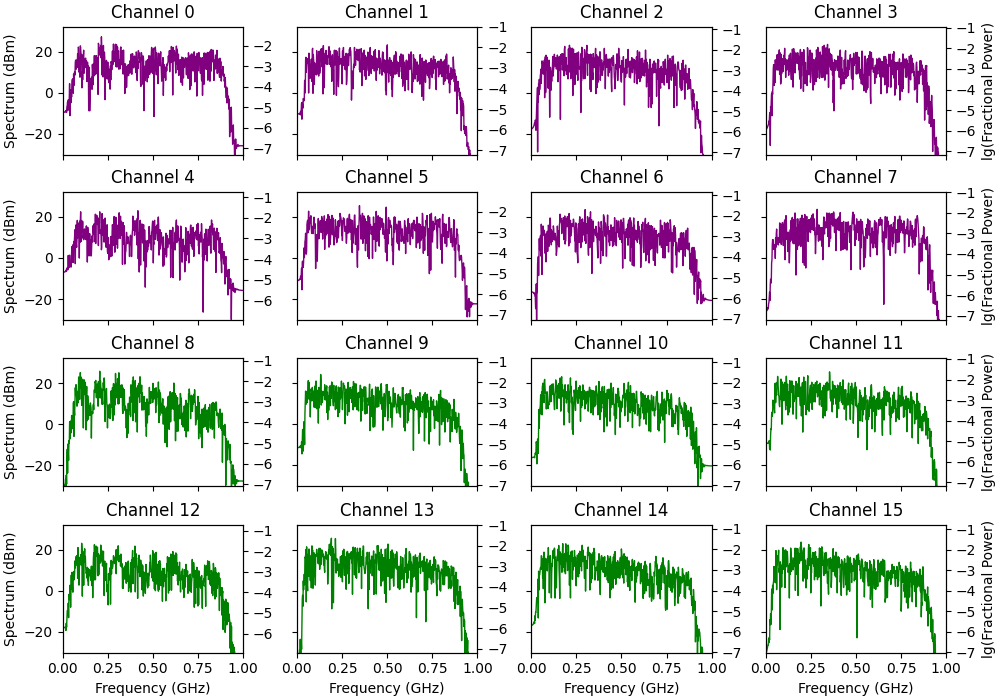
\includegraphics[width=\textwidth]{sections/5sa-cleaning/images/firstmin_station_2_run_17627_eventNo_2_spectrum.png}
      \end{subfigure}
      \caption{Example waveform (left) and spectrum (right) for an event taken within the first minute of a new run, motivating the removal of all events within the first minute of a run. This is the second event of run 17,627 of ARA2.}
      \label{fig:firstmin_waveform}
    \end{figure}
    
    % SNR or RMS vs unix time for the start of the run is not that telling. I don't remember which variables showed that the first minute of runs were bad but I'll have to remind myself
    % Myoungchul's wiki says its ADC. I'm not sure if we have anything related to ADC saved in L2 data
    % So I might have to go back to L1 data for this
    \missingfigure{2D plot showing ADC vs unixtime for the first 1 hour of a run. \label{fig:firstmin_2d}}

  \subsection{Spark Events}
  
    Another class of detector glitch backgrounds is called the Spark Event. 
    These events occur when one of the digitizing boards on the station's mainboard withstands a surge of current that inflates the digitized signal.
    Each digitizing board reads out one string for each ARA station so if one string has noticeably inflated RMS compared to the other strings, a spark event has likely taken place.
    To identify these events, the ratio in average waveform power is taken between the two strings with the greatest average power consumption. 
    Each station has a different threshold for removing an event based on this so called spark power ratio, but for ARA2 the threshold is approximately 3. 
    
    The waveform and spectrum of an example spark event is shown in Figure~\ref{fig:spark_waveform}
    
    \begin{figure}
      \centering
      \begin{subfigure}[t]{0.48\textwidth}
        \centering
        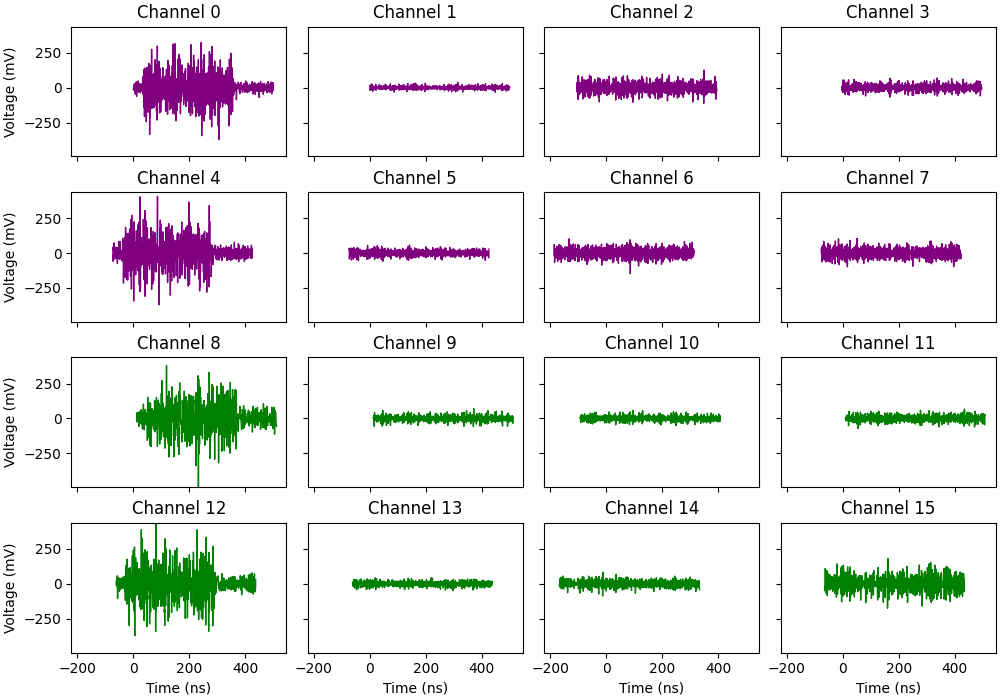
\includegraphics[width=\textwidth]{sections/5sa-cleaning/images/spark_station_2_run_7100_eventNo_1467_trace.png}
      \end{subfigure}
      ~
      \begin{subfigure}[t]{0.48\textwidth}
        \centering
        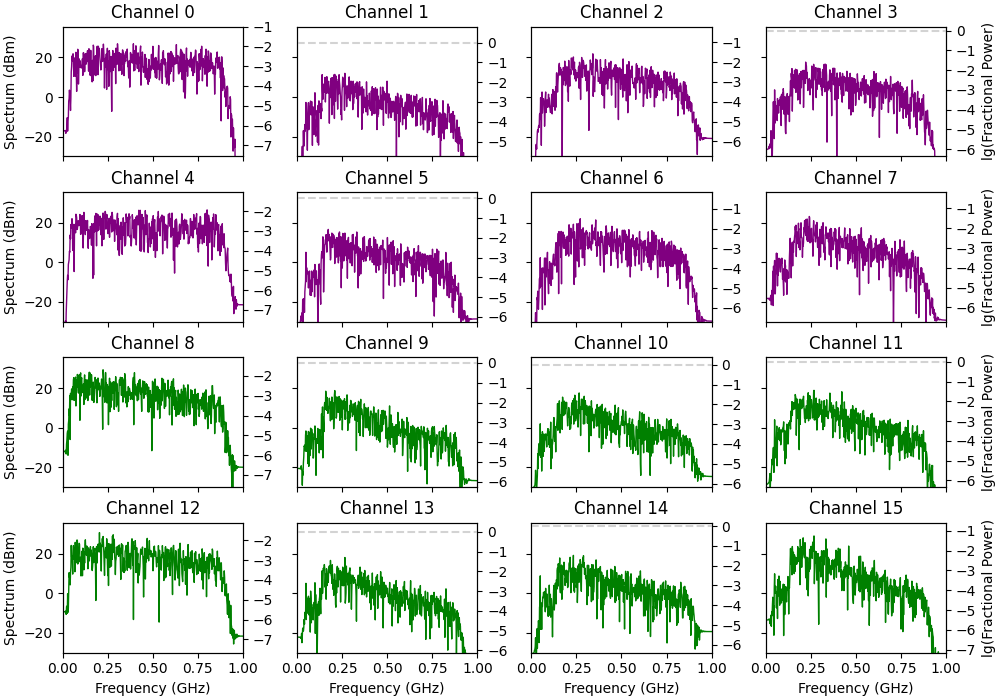
\includegraphics[width=\textwidth]{sections/5sa-cleaning/images/spark_station_2_run_7100_eventNo_1467_spectrum.png}
      \end{subfigure}
      \caption{Example waveform (left) and spectrum (right) for a spark event. Notice the significant waveform inflation in Channel 0, 4, 8, 12 (all from the same string, sharing a digitizing board) and the flattened spectrum that result from the digitizing board malfunction. This example is event 1467 of run 7100 in ARA2.}
      \label{fig:spark_waveform}
    \end{figure}

\section{Removing Anthropogenic and Science Backgrounds}

  After all erroneously digitized events are removed, events that include backgrounds we do not want to misclassify as neutrino signals must be removed. 
  This includes mis-tagged calibration pulser events, runs with known anthropogenic backgrounds, and potential cosmic ray events. 

  \subsection{Geometry Cut}
  
    The geometry cut is programmed to catch calibration pulser events that are not tagged as calibration pulser events. 
    % State how often this happens
    This may occur because the calibration pulser on a station is programmed to run once per second but it is the station's job to trigger naturally on the signals from the pulser. % Check the 1 per second bit
    The station records when the calibration pulser is firing and logs an event as a calibration event if the station triggers while the pulser is live. 
    Sometimes, calibration pulser events are not tagged as such and slip into the science dataset.
    For ARA2, events like these appear in the windows of reconstructed zenith and azimuth described in Table~\ref{tab:A2GC} on a configuration-by-configuration basis.
    The Geometry Cut enforces that events that fall within these windows are removed entirely from the analysis to remove unwanted pulser contamination from our samples.  
    
    The signals from calibration pulsers are usually recorded with strong pulses, making the interferometric reconstruction of the calpulser event obvious. 
    However pulser signals can shift in such a way that secondary solutions for the reconstruction overtake the correct solution. 
    This gives rise to populations of reconstructed calibration pulser events that are called "mirrors". 
    \missingfigure{calibration pulser mirror skymap and trace}
    \missingfigure{phi vs theta for all CP events with annotations pointing out CP5, CP5 mirror, and CP6}
    
    \begin{table}
      \centering
      \begin{tabular}{ | c | c c | c c |}
        \hline
        Object Being Cut & $\theta (^{\circ})$ & $\Delta\theta (^{\circ})$ & $\phi (^{\circ})$ & $\Delta\phi (^{\circ})$ \\
        \hline
        CP 5V & -23.5 & 4.5 & -26.35 & 4.7 \\
        CP 5V Mirror & 32.45 & 5.3 & -25.55 & 3.8 \\
        % CP 5V Mirror & 32.45 & 5.3 & -42.1 & 3.75 \\
        CP 6V & 4.5 & 5.95 & 62.9 & 6.25 \\
        \hline
      \end{tabular}
      \caption{Untagged Calibration Pulser reconstruction regions for ARA2. These cuts were inspired by the works of Myoungchul Kim from Chiba University.}
      \label{tab:A2GC}
    \end{table}
    
    To ensure that all potential untagged calibration pulser events are captured within the geometry cut, a gaussian kernel density equation is fit over the distribution of reconstructed zenith and azimuth of these events. 
    The gaussian kernel density equation was chosen by Brian Clark as the most appropriate for our data. 
    This allows us to model the tails of the reconstructed arrival directions to ensure no untagged calibration pulser events arise in our full data sample.
    
    \missingfigure{CP fits for CP5, CP5M, and CP6}
    % Should I show a plot motivating calpulser leakage? Or just cite somebody else

  \subsection{Bad Configuration Cut}
  
    Station configurations where the livetime of data, excluding bad runs, is less than 30 days are excluded from analysis. 
    Table~\ref{tab:badconfigs} shows the list of bad configurations for each station in the array. 
    Note that A2, the station focused on in this thesis, does not have any bad configurations so this cut is not applied in this thesis. 
    Due to challenges synchronizing the colocated A5 and PA instruments, A5 livetime recorded while the PA was recording are omitted to remove the possibility that duplicate events (events seen in both A5 and PA instruments) appear in the analysis. 
    Configuration 2 of A5 has more than 30 days of raw livetime, but after excluding data taken while the PA was running, A5 has less than 30 days of livetime and is therefore excluded from the analysis. 
    
    \begin{table}
      \centering
      \begin{tabular}{| c | c |}
        \hline
        Station & Bad Configurations \\
        \hline
        1 & 1 \\
        2 & None \\
        3 & None \\
        4 & 1 \\
        5 & 2 \\
        PA & 3 \\
      \end{tabular}
      \caption{Every ARA station's livetime configurations excluded from the analysis via the Bad Run Cut due to a lack of sufficient livetime. }
    \end{table}

  \subsection{Bad Run Cut}
    
    The Bad Run Cut draws directly from the Bad Run Log for the appropriate ARA station. 
    Runs are typically added to the Bad Run Log if there are known anthropogenic backgrounds present during the run. 
    This includes, but is not limited to, runs that are known to include surface pulsing calibration campaigns and heavy station activity that cannot be cleaned simply (for example, a geometry cut cannot remove snowmobile backgrounds that move in reconstructed azimuth and zenith). 
    
    Some runs can be cut due to unusual voltages in the digitizing daughter boards. \todo{explain the DDA run cut}
    Others can be cut because the station's configuration is abnormal as discussed in Section~\ref{sec:a2configs}
    
    \missingfigure{}
    
    For runs that include a large portion of anthropogenic background, it is safer to remove the entire run than to add dozens of multi-dimensional and hyper-specific cuts to remove the data. 
    The livetime reduction is not significant in doing so. 
    Brian Clark created a pipeline that systematically identifies runs with an excessive amount of outliers. 
    This pipeline takes the global maximum correlation for each RF event, plots them on a histogram, and fits two gamma Gumbel curves to the histogram. 
    The Gumbel curve is defined as % Cite Gumbel
    \begin{equation}
      f(x) = A \frac{ \beta^{\alpha} }{ \sigma ~ \Gamma(\alpha) } e^{- ( \alpha \frac{x-\mu}{\sigma} + \beta e^{({-\frac{x-\mu}{\sigma} })} ) }
      \label{eq:gumbel}
    \end{equation}
    where $A$ is a scaling factor, $\alpha=\beta$ and is initialized to 1 but free to fit, $\sigma$ is initialized as the average between the lower and upper 1$\sigma$ boundaries of the curve is called the scale parameter, and $\mu$ is initialized as peak of the histogram and called the location parameter. 
    This distribution is "suitable for modelling highly skewed and heavy-tailed data" and fits our thermal backgrounds and outliers well.  % cite http://www.kurims.kyoto-u.ac.jp/EMIS/journals/AMEN/2020/AMEN-190321.pdf and their 1st source
    The first gamma Gumbel curve is fit to the thermal background and the second is fit to the remaining outliers. 
    Examples of the gamma Gumbel curve fits to a clean and contaminated run of A2 are shown in Figure~\ref{fig:gumbel-clean} and Figure~\ref{fig:gumbel-dirty}, respectively.
    The difference between the test statistics of the Poisson negative log-likelihoods for each dual component gamma Gumbel distribution is then calculated. 
    This $\Delta TS$ parameter characterizes the separation between populations of thermal backgrounds and outliers in correlation-space. 
    A low $\Delta TS$ implies low separation and that the run is not polluted with abnormally correlated outliers. 
    A high $\Delta TS$ implies the opposite, that many events in the run are outliers in the regime of global max correlation. 
    A histogram of the $\Delta TS$ values for each run in each station's livetime configuration is plotted. 
    A run-level cut based on the value of $\Delta TS$ for the run is determined based on the presence of runs with copious outliers compared to the distribution of runs that are predominately thermal as shown in Figure~\ref{fig:deltaTS-per-config}. 
    
    \missingfigure{Gumbel for a clean run in A2 \label{fig:gumbel-clean}}
    \missingfigure{Gubmel for an outlier-y run in A2 \label{fig:gumbel-dirty}}
    \missingfigure{Distribution of gumbel curves for each config of A2 \label{fig:deltaTS-per-config}}
    
    
  \subsection{Spatio-Temporal Cut}
  
    Any anthropogenic background that is not removed by the Bad Run Cut is likely to be removed by the spatio-temporal cut. 
    
  \subsection{Zenith Cut}
  
    The Zenith Cut is employed at the end of the cleaning pipeline to remove any remaining anthropogenic surface events, such as continuous wave contaminated events that weren't fully filtered, and cosmic ray events. 
    The cosmic ray events that ARA can observe typically result from an ultra high energy cosmic ray (UHECR) interacting in the atmosphere, causing an airshower, and potentially impacting into the ice. 
    Depending on the energy and direction the UHECR is traveling in, an ARA station may see radio signals from the air shower portion and/or the ice-impacting core. 
    % Cite Nicolas, maybe show photos
    The Zenith Cut is harsh and strict and is employed last so that other cuts can be tuned as much as possible to remove backgrounds. 
    Continuous Wave contamination interferes with the reconstruction of a signal and can therefore make a surface event reconstruct in the ice. 
    Relying on the zenith cut to remove all surface related backgrounds is risky for this reason and should be employed near the end of cleaning. 
    
    We employ a conservative zenith cut at 0 degrees in elevation to ensure that all surface events are removed from the analysis. 
    
  \subsection{Low Reconstruction Confidence Cut}
    
    For the few remaining events, they are cleaned up using 
  
  % solar activity? 
  
\section{Employment of Cuts and Impact on Potential Neutrino Events}

  The cuts are applied to A2 data in the following order: 
  \begin{enumerate}
    \item Bad Run Cut
    \item Spark Event Cut
    \item Geometry Cut
    \item Spatio-Temporal Cut
    \item Zenith Cut
    \item Low Reconstruction Confidence Cut
  \end{enumerate}

  \missingfigure{For each configuration: efficiencies, snr-vs-corr for noise, neutrinos with no and all cuts, data with no and all cuts.}
  
  
  
  
  
  
\chapter{The Askaryan Radio Array's Five Station Analysis \label{chap:5sa_analysis}}

  After reducing our 10\% data to a predominantly thermal-like collection of events, we construct an analysis that separates potential signal from our background. 
  This is done by training a Linear Discriminant Analysis (LDA) algorithm on each station-configuration.
  The LDA determines the linear projection of the data that provides the best separation between signal and background relative to their statistical spread, discussed further in Section~\ref{sec:lda}.
  The distribution of LDA values for thermal-like events is modeled and passed, along with the model of surface-like events identified in Section~\ref{sec:zc_slc}, to an optimization algorithm that identifies the best LDA cut for each station-configuration in the context of each array-wide configuration and the best Zenith Cut for the 6 instruments. 
  The optimization is explained in Section~\ref{sec:optimization}.

  Once the LDA cut (discriminating signal from background) and the Zenith Cut (rejecting cosmic rays and unparameterized anthropogenic noise) are optimized based on the 10\% sample and simulated neutrino events, the analysis is applied to the 100\% dataset. 
  Post-unblinding, we assess the compatibility of the models built on the 10\% data which drove the optimized LDA Cut and Zenith Cut are compared with the now-unblinded 100\% data.
  Any events that survive all analysis cuts (cleaning and LDA) are then passed through an isolation condition that removes any events that occurred between 5 seconds and 5.8 hours of each other, as we don't expect to find multiple neutrino events in close succession, except events that observe multiple particles or cascades (muon and tau tracks of stochastic losses and a tau decay), like those quantified in Fig.~\ref{fig:secondaries_contribution}. 
  We outline a plan for how to assess any remaining (``passing'') events, in case they are due to unforeseen backgrounds not present in the 10\% sample. 
  Lastly, we use the expected background rates and the number of passing events to establish an upper limit on the flux of UHE neutrinos. 

\section{The Linear Discriminant Analysis \label{sec:lda}}

  In this analysis, thermal background discrimination from expected neutrino signal is performed using a Linear Discriminant Analysis (LDA).
  Previous analyses have used the Fisher Discriminant~\citep{fisherDiscriminant, ara_pa_analysis} or a cut in the 2 dimensional distribution of event correlation against signal strength~\citep{ara_a23}. 
  An LDA is a generalization of Fisher Discriminants and, if only using two variables, performs similarly to separating signal and background by drawing a line in the 2 dimensional histogram of event correlation versus signal strength. 
  LDAs, for each event, will take an array of analysis variables and combine them linearly into a single number by multiplying the variables for each event against a matrix that's been optimized to minimize LDA scores for background events and maximize scores for signal events. 
  This analysis uses the 19 variables summarized in Table~\ref{tab:LDAvars} to train the LDA. 
  These 19 variables are chosen based on their ability to distinguish thermal-like events from neutrino events while minimizing correlations between the variables.
  This LDA is trained on a signal dataset composed of simulated neutrino events following the global experimental upper limit on the cosmic neutrino set (defined by Ref.~\citep{icecube_search-ehe} and Ref.~\citep{anita_iv}), and a background dataset composed of all events from each station's cleaned 10\% sample.   
  
  \begin{table}
    \centering
    \resizebox{0.9\textwidth}{!}{ % Shrink the table since it overflows a bit
      \begin{tabular}{c | p{0.8\linewidth} }
        Variable Name & Definition \\
        \hline
        \texttt{global\_max\_corr} & Maximum correlation score between all waveforms \\
        \texttt{global\_max\_corr\_v} & Maximum correlation score between waveforms from VPol antennas\\
        \texttt{global\_max\_corr\_h} & Maximum correlation score between waveforms from HPol antennas\\
        \texttt{avg\_snr\_v} & Average SNR of signals from VPol antennas \\
        \texttt{avg\_snr\_h} & Average SNR of signals from HPol antennas \\
        \texttt{hilbert\_snr\_v} & Average Hilbert Enveloped SNR of signals from VPol antennas \\ 
        \texttt{corr\_snr\_v} & Average SNR of the correlation function between all pairs of VPol antennas \\
        \texttt{csw\_snr\_v} & Coherently Summed Signal to Noise Ratio  in VPol antennas \\
        \texttt{avg\_rpr\_v} & Average SNR of signal power in VPol antennas \\ % Get a better definition
        \texttt{csw\_rpr\_v} & SNR of the power in the CSW from signals in VPol antennas \\ % Get a better definition
        \texttt{impulsivity\_v} & Power consumption during period maximal power consumption in the CSW compared to the rest of the CSW \\
        \texttt{bImp\_v} & Y-intercept of the linear fit to the latter portion of the impulsivity curve\\
        \texttt{mImp\_v} & Slope of the linear fit to the latter portion of the impulsivity curve \\
        \texttt{rhoImp\_v} & R-value of the linear fit to the latter portion of the impulsivity curve\\
        \texttt{impLinChi2\_v} & Difference between the linear fit to the latter portion of the impulsivity curve and a perfectly non-impulsive curve with a slope of 1. \\
        \texttt{impErfA\_v} & $A$ term in the functional fit to the impulsivity curve given by Equation~\ref{eq:functionalimp} \\
        \texttt{impErfB\_v} & $B$ term in the functional fit to the impulsivity curve given by Equation~\ref{eq:functionalimp} \\
        \texttt{impErfLinChi2\_v} & $\chi^2$ of the functional fit to the impulsivity curve given by Equation~\ref{eq:functionalimp} \\
        \texttt{impSig\_v} & Significance of the functional impulsivity fit given by Equation~\ref{eq:functionalimp} compared to the linear fit via Wilk's Theorem \\
      \end{tabular}
    }
    \caption{
        Analysis Variables used in the Linear Discriminant analysis along with a short description. 
        Full definitions of each variable can be found in Appendix~\ref{app:5savariables}.
    }
    \label{tab:LDAvars}
  \end{table}

  \begin{figure}
      \centering
      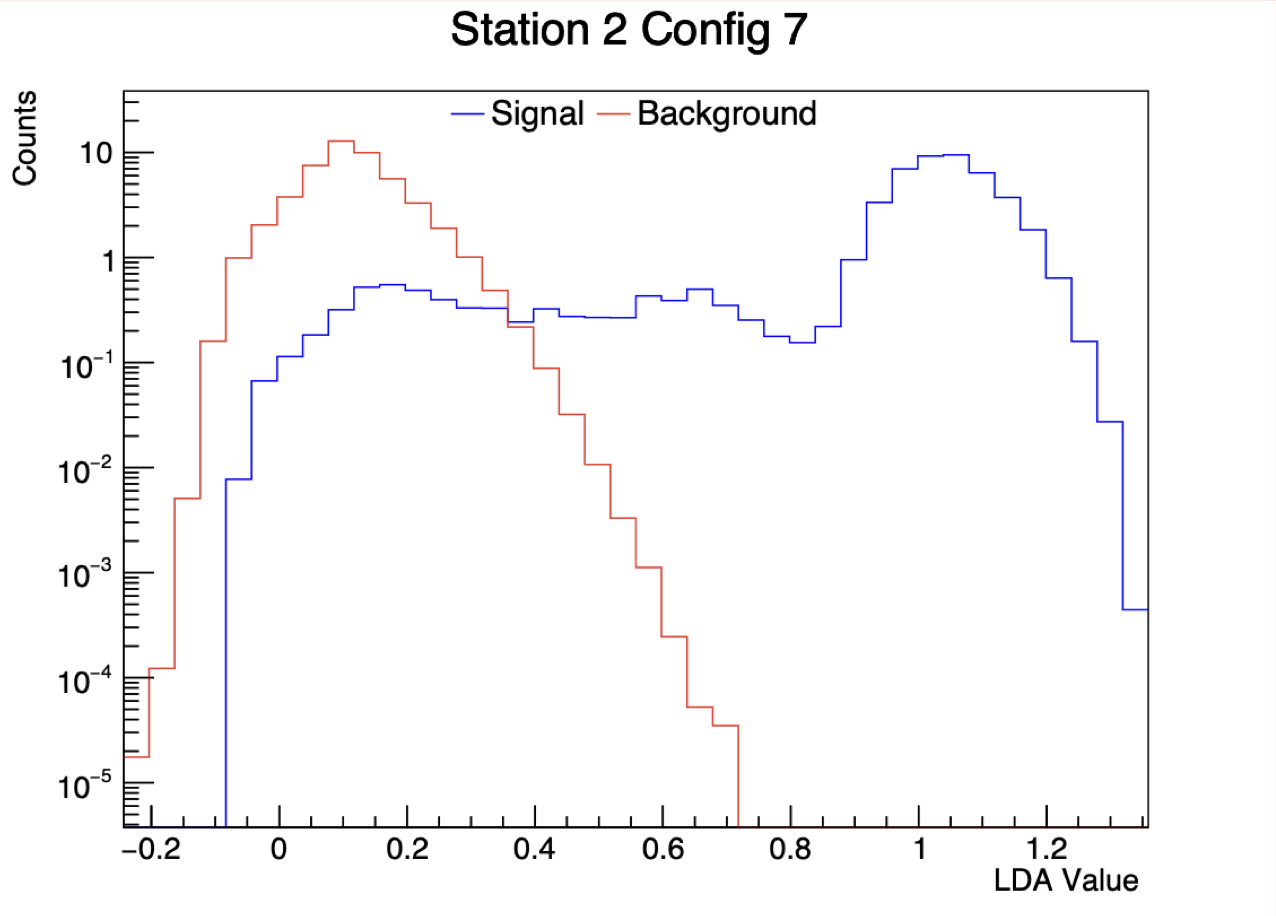
\includegraphics[
          width=0.75\textwidth,
          alt={}
      ]{sections/5sa-analysis/images/a2c7_lda_nudata.png}
      \caption{
        Distribution of Linear Discriminant Analysis scores for thermal-like background events (red, RF triggers that pass all cuts designed in Chapter~\ref{chap:5sa_cleaning}) from the 10\% sample and simulated neutrinos (blue) in A2 configuration 7.
      }
      \label{fig:ldafit}
  \end{figure}

  \begin{figure}
    \centering
    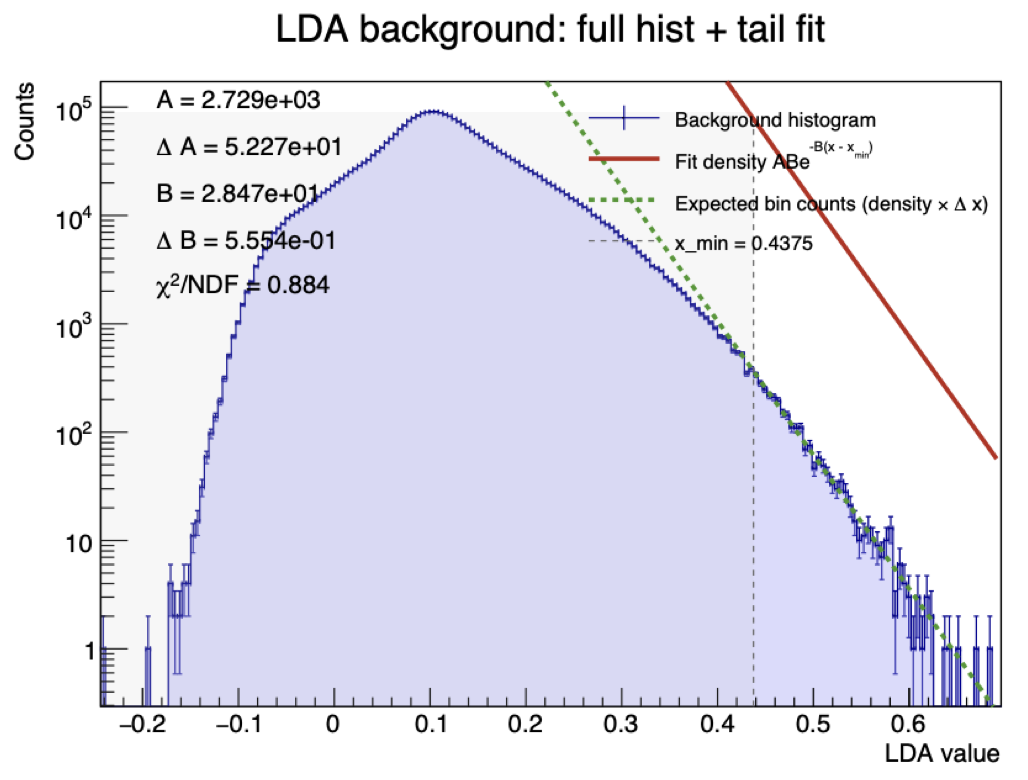
\includegraphics[
        width=0.75\textwidth,
        alt={}
    ]{sections/5sa-analysis/images/a2c7_10pct_lda_backgroundfit.png}
    \caption{
      Distribution of Linear Discriminant Analysis scores for the thermal-like background events (blue, RF triggers that pass all cuts designed in Chapter~\ref{chap:5sa_cleaning}) in the 10\% sample and from A2 configuration 7 fitted to an exponential (green).
      The fit is performed only on data $\geq x_{\text{min}}$.
      The fit is performed over a scan of $x_{\text{min}}$ values and the fit with the best reduced-$\chi^2$ is selected.
      The red curve shows the fit density (green line divided by the bin width, $\Delta x$).
    }
    \label{fig:backgroundfit_10pct}
  \end{figure}

  Once the LDA transformation matrix is optimized to separate thermal-like background events from neutrino events, we plot the LDA distributions for the signal and background datasets as show in Fig.~\ref{fig:ldafit}. 
  High statistics samples show that the tail of this distribution can be characterized by an exponential 
  \begin{equation}
    f(x) = A e^{-B (x-x_{\text{min}})}
    \label{eq:backgroundfit_exp}
  \end{equation}
  We fit the upper tail of the background event LDA distribution to this form and use it in the upcoming array-wide optimization. 
  In this context, $x$ is the central LDA value of the bin, $x_{\text{min}}$ is the LDA value above which the fitting is performed, and $A$ and $B$ are fit parameters. 
  An example of this fit is shown in Fig.~\ref{fig:backgroundfit_10pct} for the A2 configuration 7 thermal background LDA distribution. 

  We assess the integrity of the background tail fit via pseudoexperiments\index{Pseudoexperiment}.
  These pseudoexperiments use Poisson statistics to re-sample the LDA distribution shown in Fig.~\ref{fig:backgroundfit_10pct} according to a modified tail fit that has been subjected to Gaussian fluctuations.
  Variations in the model fit parameters characterize systematic uncertainties on the background model while re-sampling the LDA distribution characterizes statistical uncertainties. 
  Enumerated, this procedure is as follows: 
  \begin{enumerate}
    \item The parameters $A$ and $B$ in Eq.~\ref{eq:backgroundfit_exp} of the exponential tail model that was fit to real thermal background LDA values are re-sampled according to Gaussian fluctuations, obtaining a ``temporary" tail model. The fit error for $A$ and $B$ established when fitting the real thermal background model define the Gaussian widths for the fluctuations.
    \item For each bin in the LDA distribution, the temporary tail model is integrated over the bin to obtain a number of counts in the bin. This number of counts is then re-sampled following Poisson statistics.
    \item The log-likelihood of this re-sampled LDA distribution is calculated with respect to the original thermal background model.
    \item The above three steps are repeated 10,000 times and a distribution of log-likelihoods is plotted as shown in Fig.~\ref{fig:backgroundfit_10pct_toys}. The log-likelihood of the real observed distribution is also calculated with respect to the original thermal background model and plotted for reference. The fraction of toys with a log-likelihood greater than the observed log-likelihood (the p-value) is reported. 
  \end{enumerate}

  \begin{figure}
    \centering
    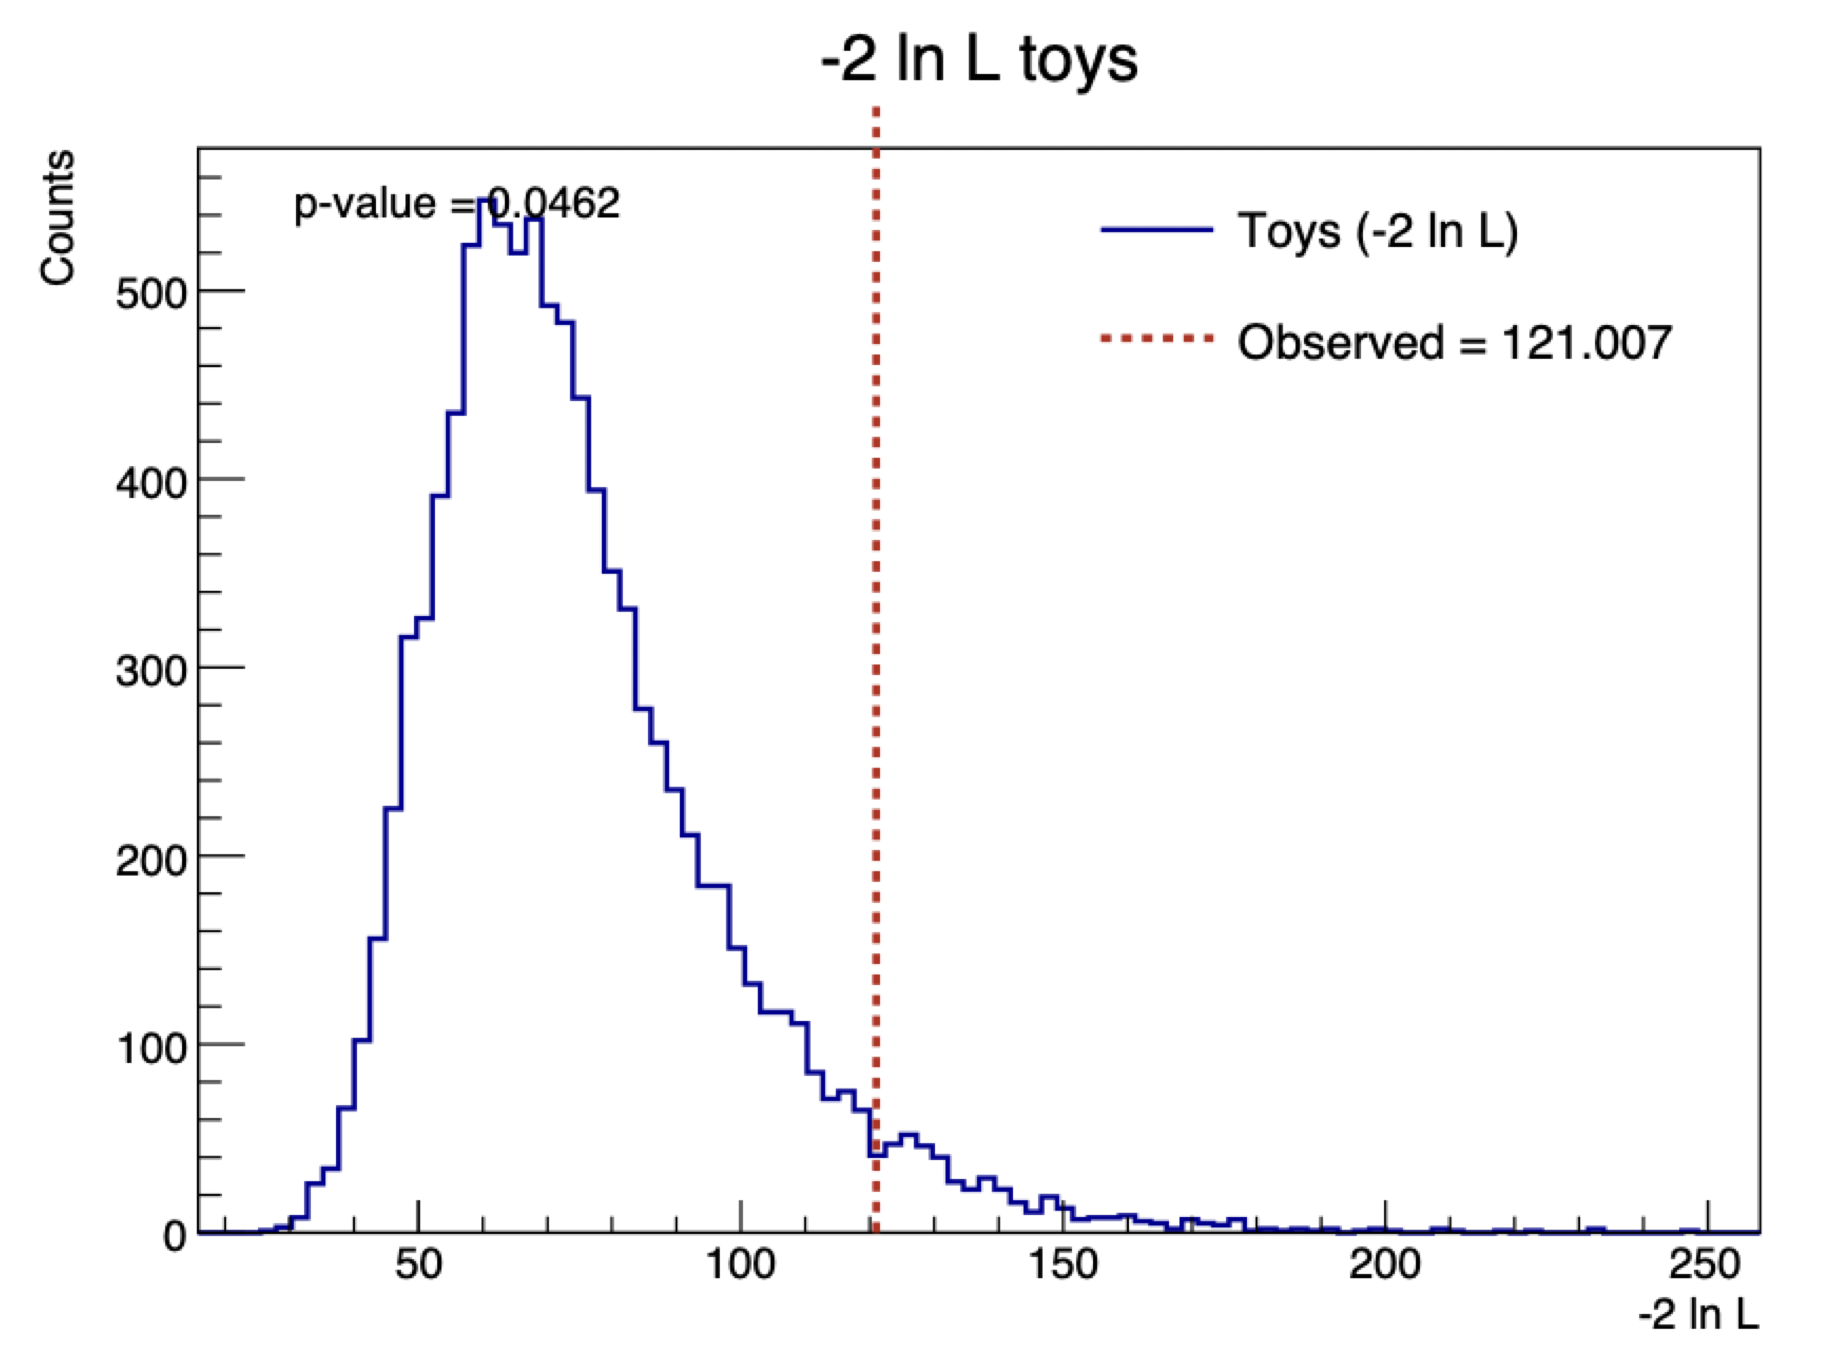
\includegraphics[
        width=0.75\textwidth,
        alt={}
    ]{sections/5sa-analysis/images/a2c7_100pct_lda_backgroundfit_toys.png}
    \caption{Distribution of log-likelihoods comparing background pseudoexperiments (blue) to the background model on observed 100\% A2 configuration 7 data (red).}
    \label{fig:backgroundfit_10pct_toys}
  \end{figure}

  At the end of this process, we have models of background LDA values for each station and configuration which will be combined for array-wide optimization.
  Note that as the LDA transformation matrix is optimized separately for each station-configuration, the resulting LDA scores for each station-configuration should not be compared to each other. 
  Said another way, if one station-configuration's LDA distribution ends at 1.2 and another ends at 1.4, this does not simply imply the former is better than the latter. 

\section{Optimization \label{sec:optimization}}

  After the thermal background LDA model determined in Section~\ref{sec:lda} and the surface event elevation models determined in Section~\ref{sec:zc_slc} for each station-configuration are set, we feed them both into an algorithm that determines the best LDA cut and Zenith Cut for each array-wide configuration. 
  An array-wide configuration is defined by the combination of active stations (in their respective station livetime configuration) over time periods of at least 1 week. 
  There are 50 total array-wide combinations of the 29 total station configurations, as shown in Fig.~\ref{fig:ARA_configurations}.
  Each LDA cut is established within each array-wide configuration. 
  For example, A2 configuration 7 is present in array-wide configurations 40, 42, 43, and 44 and has a different LDA cut optimized for each array-wide configuration in the parameter space of the same parent distribution.
  Expanding on this, across the full 50 array-wide configurations there are 144 LDA cuts to establish using the same 29 parent datasets. 
  We optimize just one zenith cut for each station (there are not enough statistics to do it based on station configuration like with the LDA).
  In total this results in 6 Zenith Cuts and 144 LDA Cuts to be optimized.
  The optimized A2 Zenith Cut is set to an elevation angle of $10.31^{\circ}$ and the minimum and maximum LDA cut for each A2 configuration are presented in Table~\ref{tab:ldacuts}. 
  The signal efficiency of the analysis over the entire array is plotted as a function of simulated neutrino energy in Fig.~\ref{fig:LDA_efficiency_wLDA} with the optimized LDA applied.

  \begin{table}
    \centering
    \begin{tabular}{cc}
      Livetime Configuration & LDA Cut Range \\
      \hline
      1 & 0.95 - 0.99 \\
      2 & 1.14 \\
      3 & 0.90 - 0.91 \\
      4 & 1.01 - 1.02 \\
      5 & 1.15 - 1.34 \\
      6 & 1.11 - 1.23 \\
      7 & 0.97 - 1.00 \\
    \end{tabular}
    \caption{
      Range of cuts used to distinguish thermal background events from neutrino signal events, after optimization. 
    }
    \label{tab:ldacuts}
  \end{table}

  \begin{figure}
    \centering
    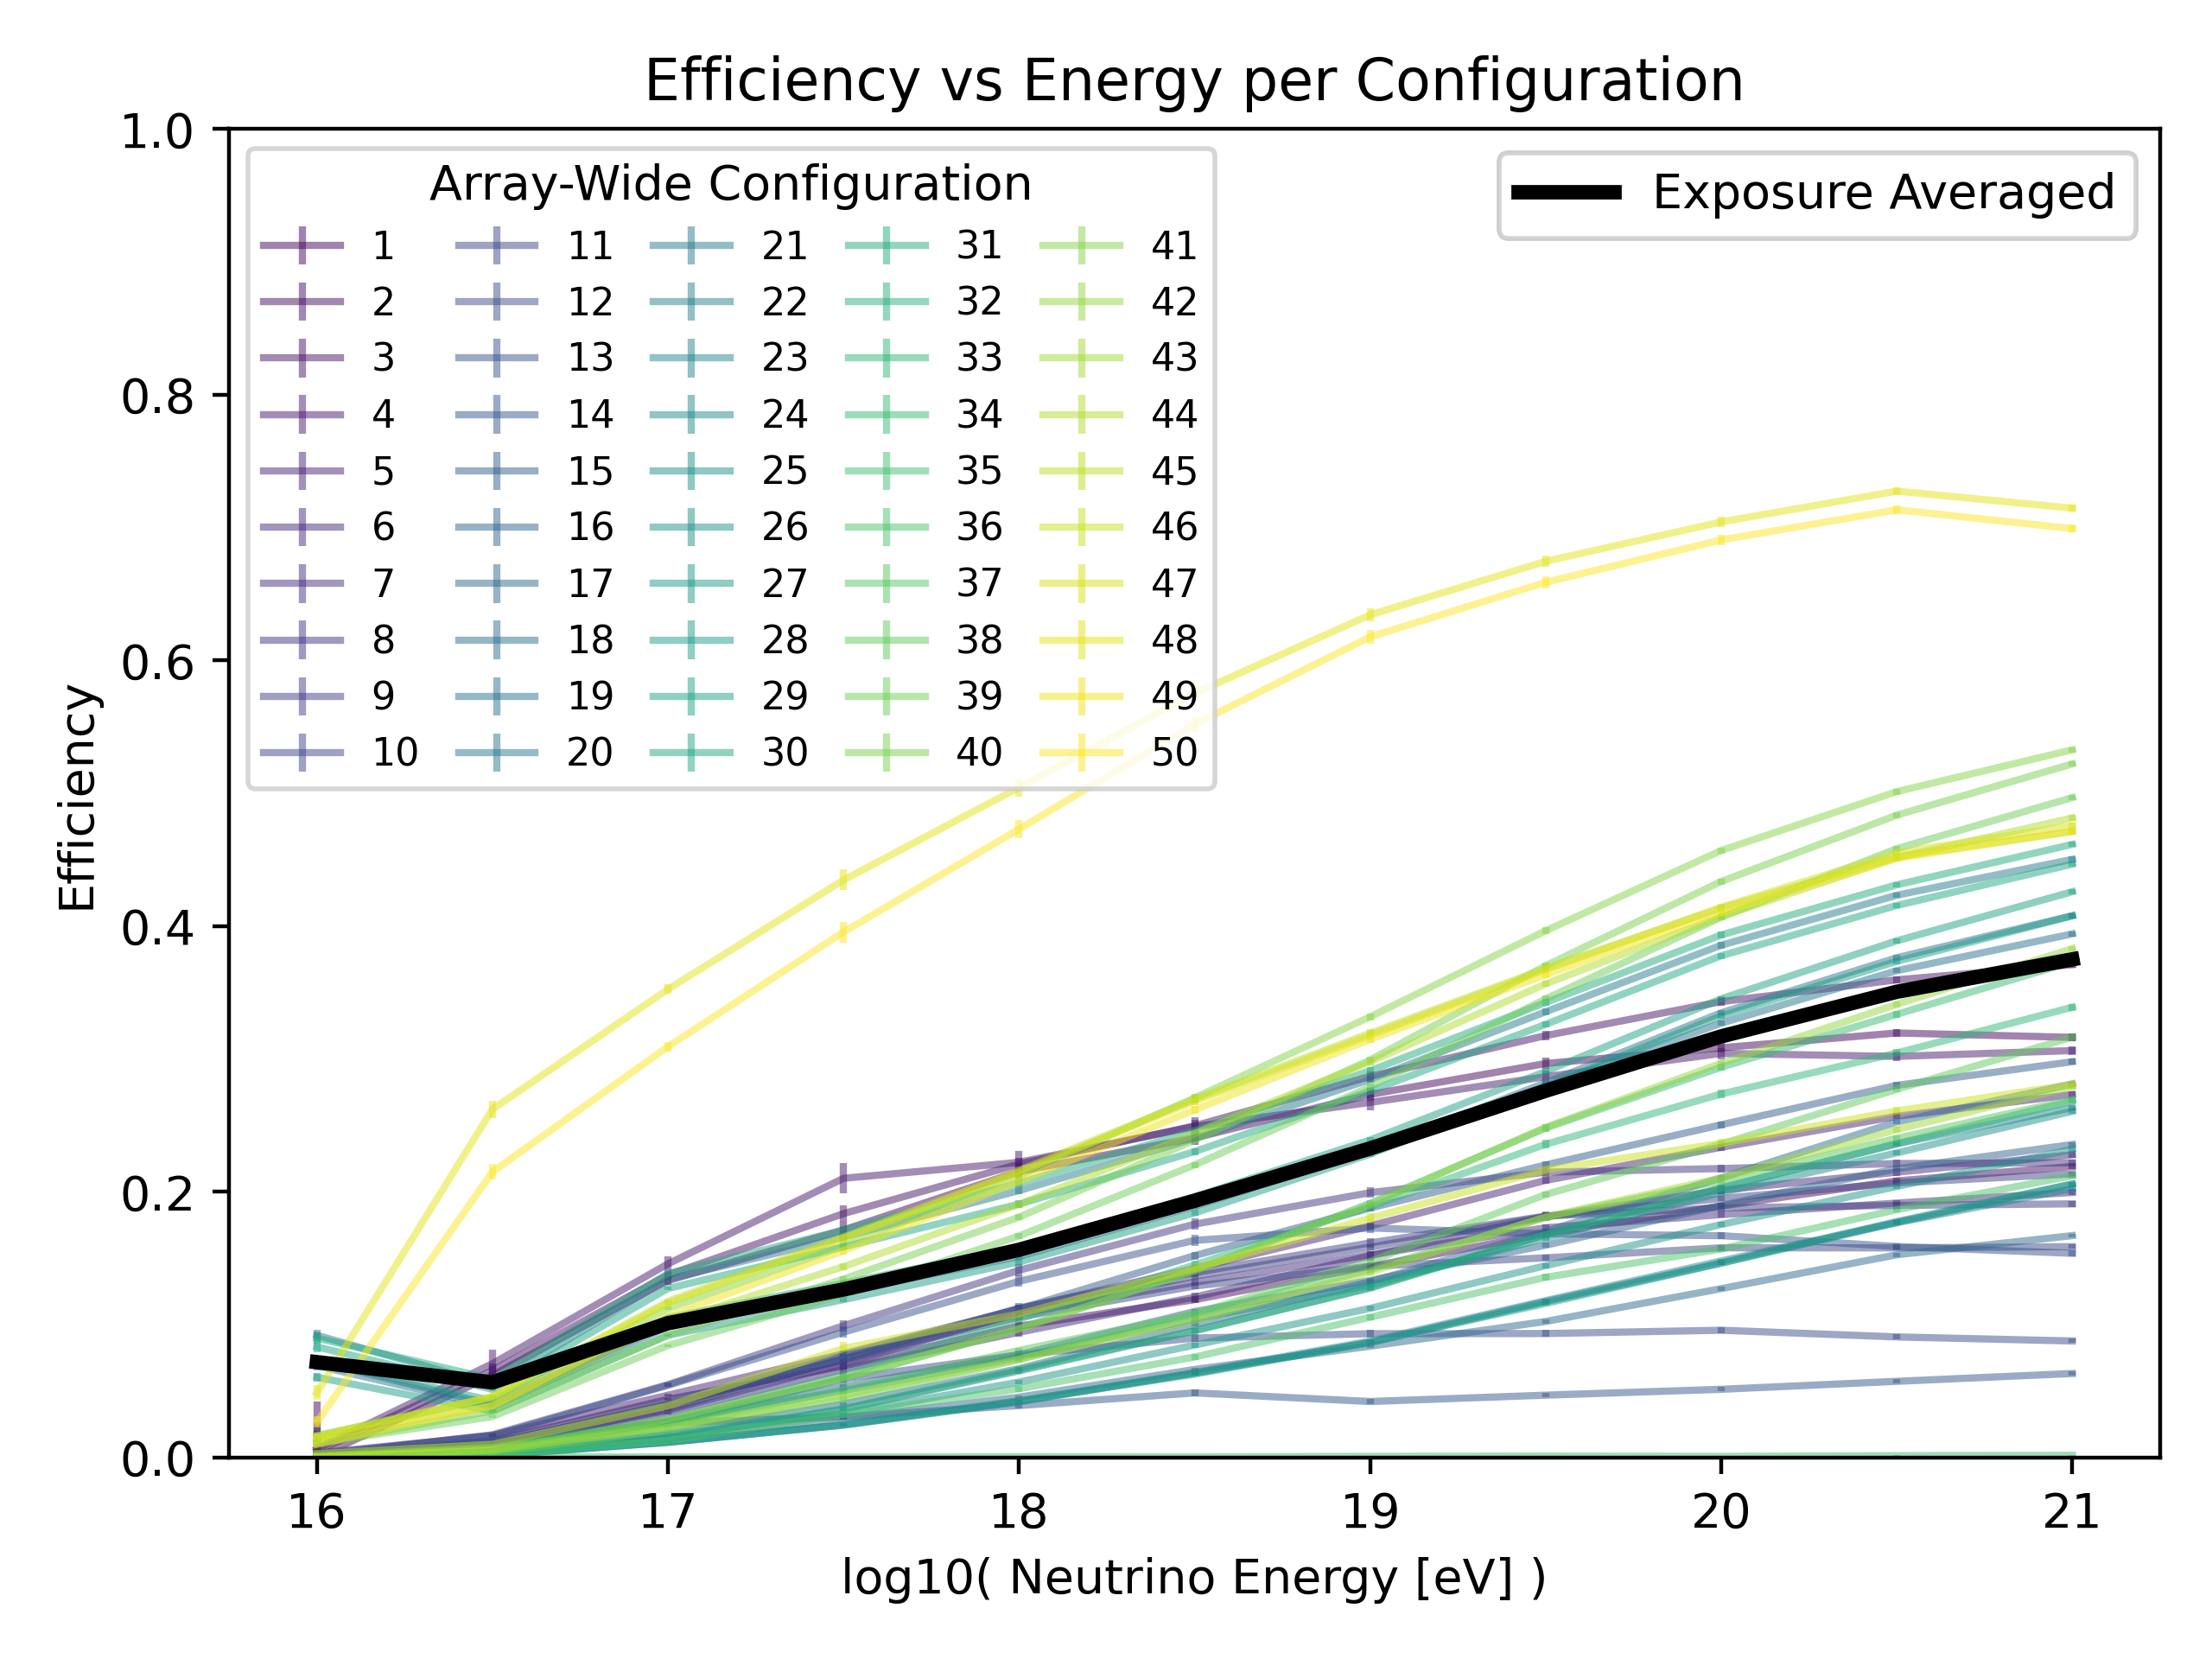
\includegraphics[
      width=0.7\linewidth,
      alt={}
    ]{sections/5sa-analysis/images/arraywide_efficiencies_vs_energy.png}
    \caption{
      Array-wide signal efficiency for each array-wide configuration (colored lines) and the exposure-weighted efficiency over all array-wide configurations (black lines) presented as a function of neutrino energy. 
      The two lines with the greatest signal efficiency are for array-wide configuration 48 and 50 during both of which, only the PA was active therefore demonstrating the signal efficiency of the PA detector in isolation.
      This represents the array-wide signal efficiency after all cleaning cuts defined in Chapter~\ref{chap:5sa_cleaning} were applied (using Zenith Cuts and Surface Like Cuts optimized in this section) and after the optimized LDA cut was applied.
    }
    \label{fig:LDA_efficiency_wLDA}
  \end{figure}

\section{Post-Unblinding Analysis \label{sec:unblinding}}

  Running the analysis pipeline over the full 100\% data and viewing which events survived all cuts for the first time is commonly referred to as ``opening the box". 
  After opening the box we investigate any events that pass the analysis and construct our analysis' sensitivity to UHE neutrinos.
  But, before we analyze the full data sample, we ensure that the surface background elevation model and the thermal background LDA model constructed with the 10\% dataset and used to establish the final Zenith and LDA Cuts are compatible with the 100\% data. 
  There is also one final cut to remove any array-wide temporal clusters of events which removes events that occur array-wide called the Time Isolation Cut.

  \subsection{Surface Cut Cross Checks}

    \begin{figure}
      \centering
      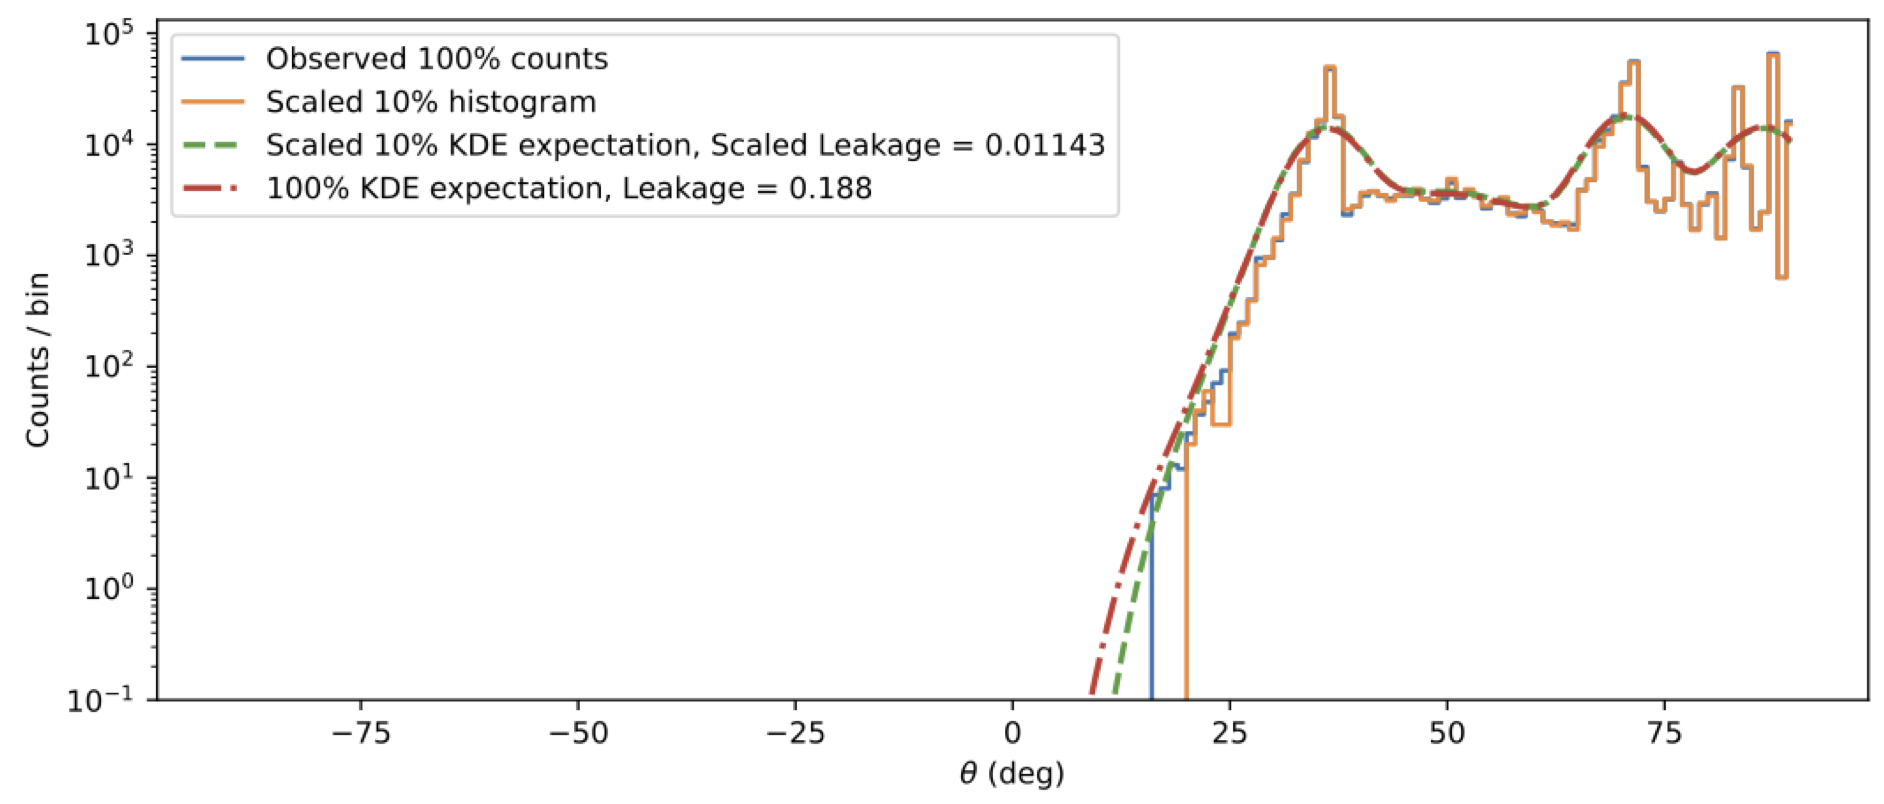
\includegraphics[
          width=\textwidth,
          alt={}
      ]{sections/5sa-analysis/images/a2_100pct_surfacecheck_zenithdist.png}
      \caption{
        The A2 surface background dataset built with the 10\% data and multiplied by 10 (orange) is compared to the surface background dataset built with the 100\% data (blue), as described in Section~\ref{sec:zc_slc}.
        The background model built on the 10\% dataset multiplied by 10 (green) compared to a model built on the 100\% dataset (red).
        The number of events that pass this cut is calculated as the number of events calculated using the red 100\% KDE line with an elevation angle below the optimized Zenith Cut of $10.31^{\circ}$.
      }
      \label{fig:backgroundcheck_zenith_dist}
    \end{figure}

    The first post-unblinding check is to build a surface event dataset and model (as described in Section~\ref{sec:zc_slc}) using the 100\% datasets then compare it to the model built with the 10\% data. 
    The distribution of event elevations in the surface dataset built with 100\% data is shown in Fig.~\ref{fig:backgroundcheck_zenith_dist} which shows strong visual agreement between the model built on the 10\% and the 100\% datasets. 
    All events in the 100\% distribution that have an elevation less than the lowest bin edge from the 10\% distribution have a \texttt{mindepth\_v} score greater than -5~m.
    This means that each event's highest reconstructed source origin (within 300~m) with a reconstruction correlation score at least 60\% of the all-sky maximum is at least -5~m. 
    Events originating from the surface have similar \texttt{mindepth\_v} scores.

    % \begin{figure}
    %   \centering
    %   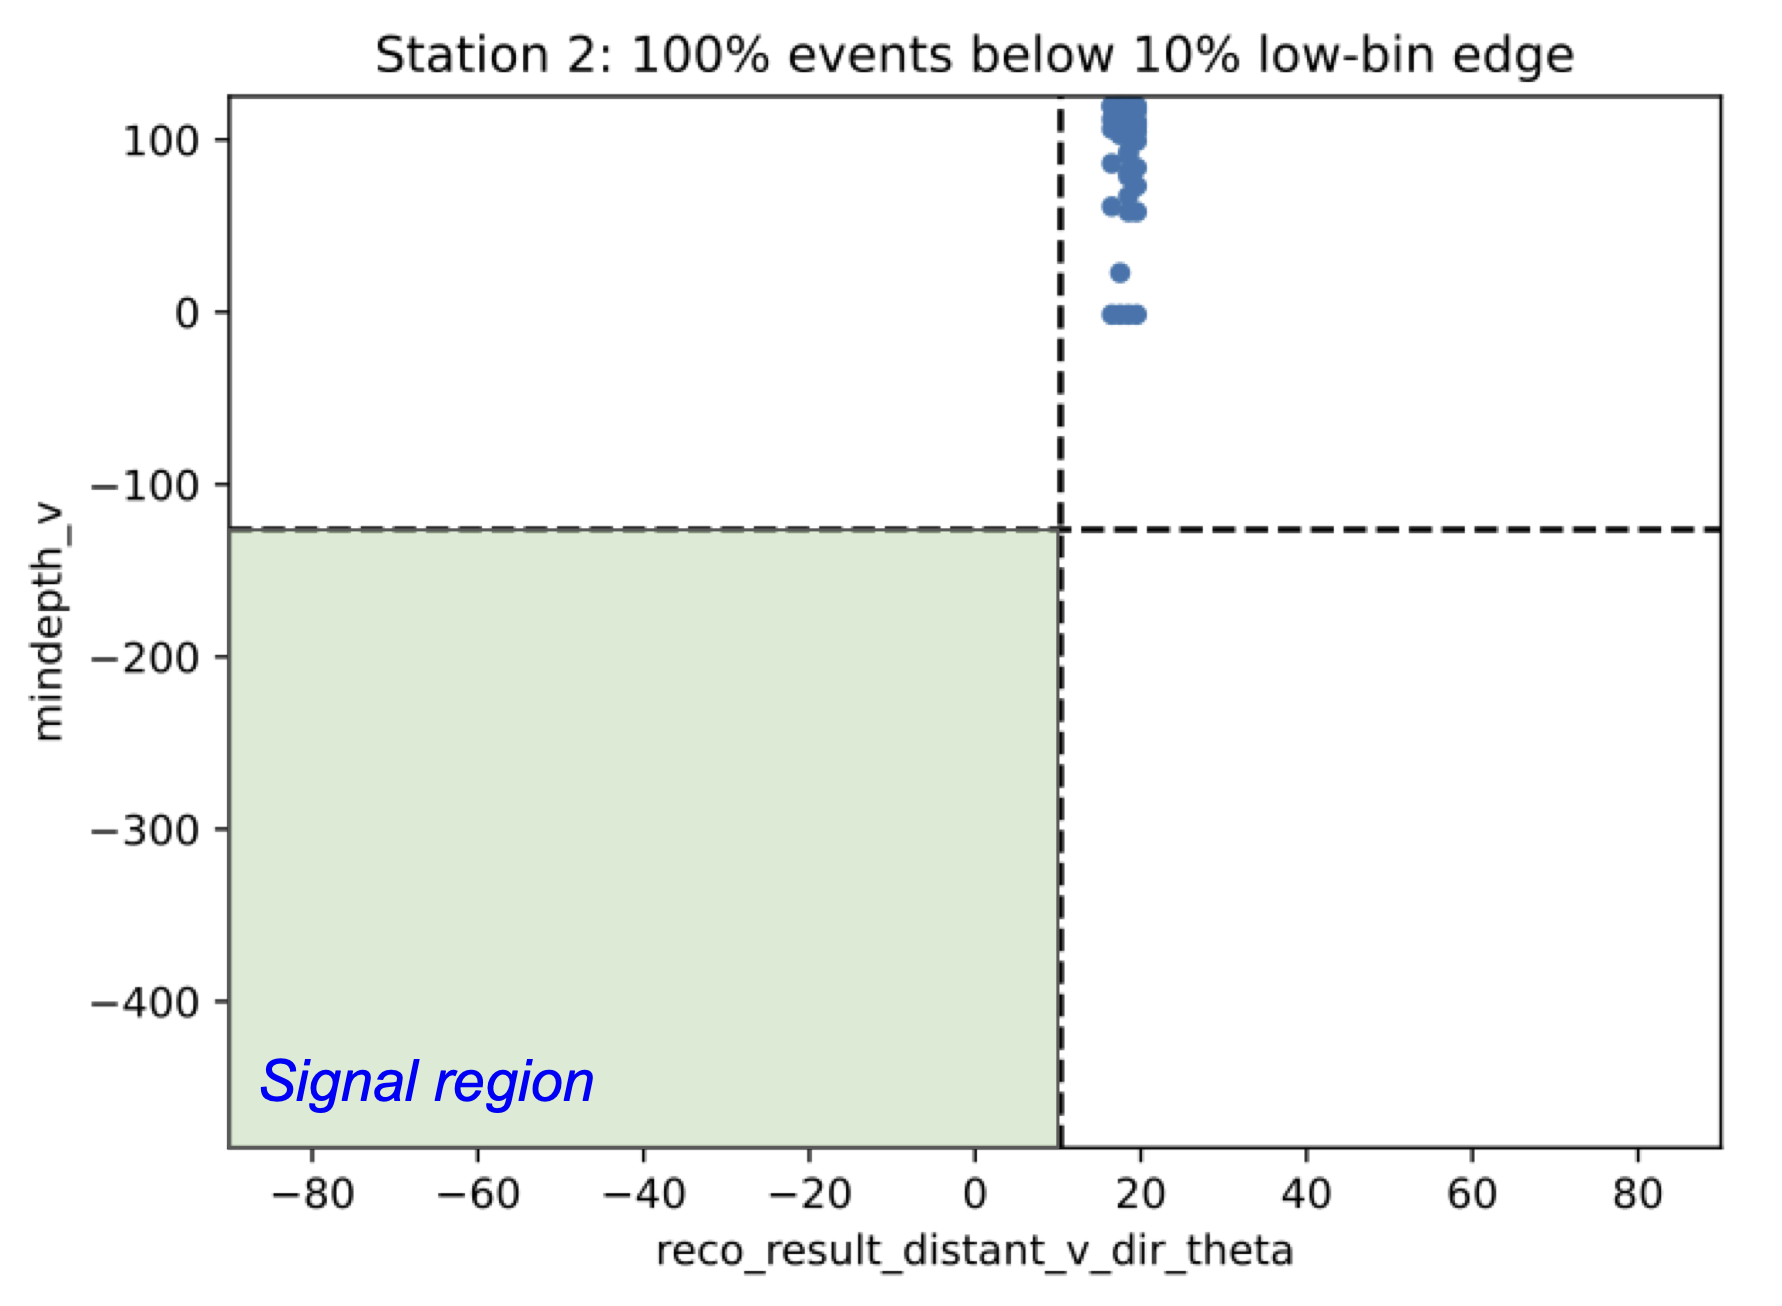
\includegraphics[
    %       width=0.75\textwidth,
    %       alt={}
    %   ]{sections/5sa-analysis/images/a2_100pct_surfacecheck_outliers.png}
    %   \caption{
    %     Distribution of events from the full 100\% dataset with reconstructed elevations less than the lowest bin in the 10\% dataset (as shown in Fig.~\ref{fig:backgroundcheck_zenith_dist}) plotted by their reconstructed elevation and \texttt{mindepth\_v}.
    %     As these events all have a \texttt{mindepth\_v} value sufficiently above the \texttt{mindepth\_v} cut established by the Zenith Cut optimization, these outliers do not suggest we have not modeled our surface background too loosely.
    %   }
    %   \label{fig:backgroundcheck_zenith_outliers}
    % \end{figure}

    % The 2 dimensional distribution of \texttt{mindepth\_v}\index{\texttt{L2 Variable: mindepth\_v}} and reconstructed elevations for events in the 100\% dataset that reconstruct below $20^{\circ}$, the lowest bin in the 10\% dataset, is shown in Fig.~\ref{fig:backgroundcheck_zenith_outliers}. 
    % The \texttt{mindepth\_v} parameter describes the minimum depth (converted from elevation angle) where the correlation score of an event's reconstruction is at least 60\% of the full reconstruction's maximum correlation score. 
    % Higher values of \texttt{mindepth\_v} indicate higher probabilities that an event originated from near and above the surface of the ice, where our data sample is largely contaminated by anthropogenic backgrounds and cosmic ray events.
    % This plot was created to ensure that none of these events in the 100\% surface data set with a reconstructed elevation less than $20^{\circ}$ were likely to have originated in the ice where we are searching for neutrinos. 
    % Figure~\ref{fig:backgroundcheck_zenith_outliers} shows that all of these events had a \texttt{mindepth\_v} of at least -1.7~m - meaning these events all had a high probability of originating near or above the surface and do not invalidate our background model.

    \begin{figure}
      \centering
      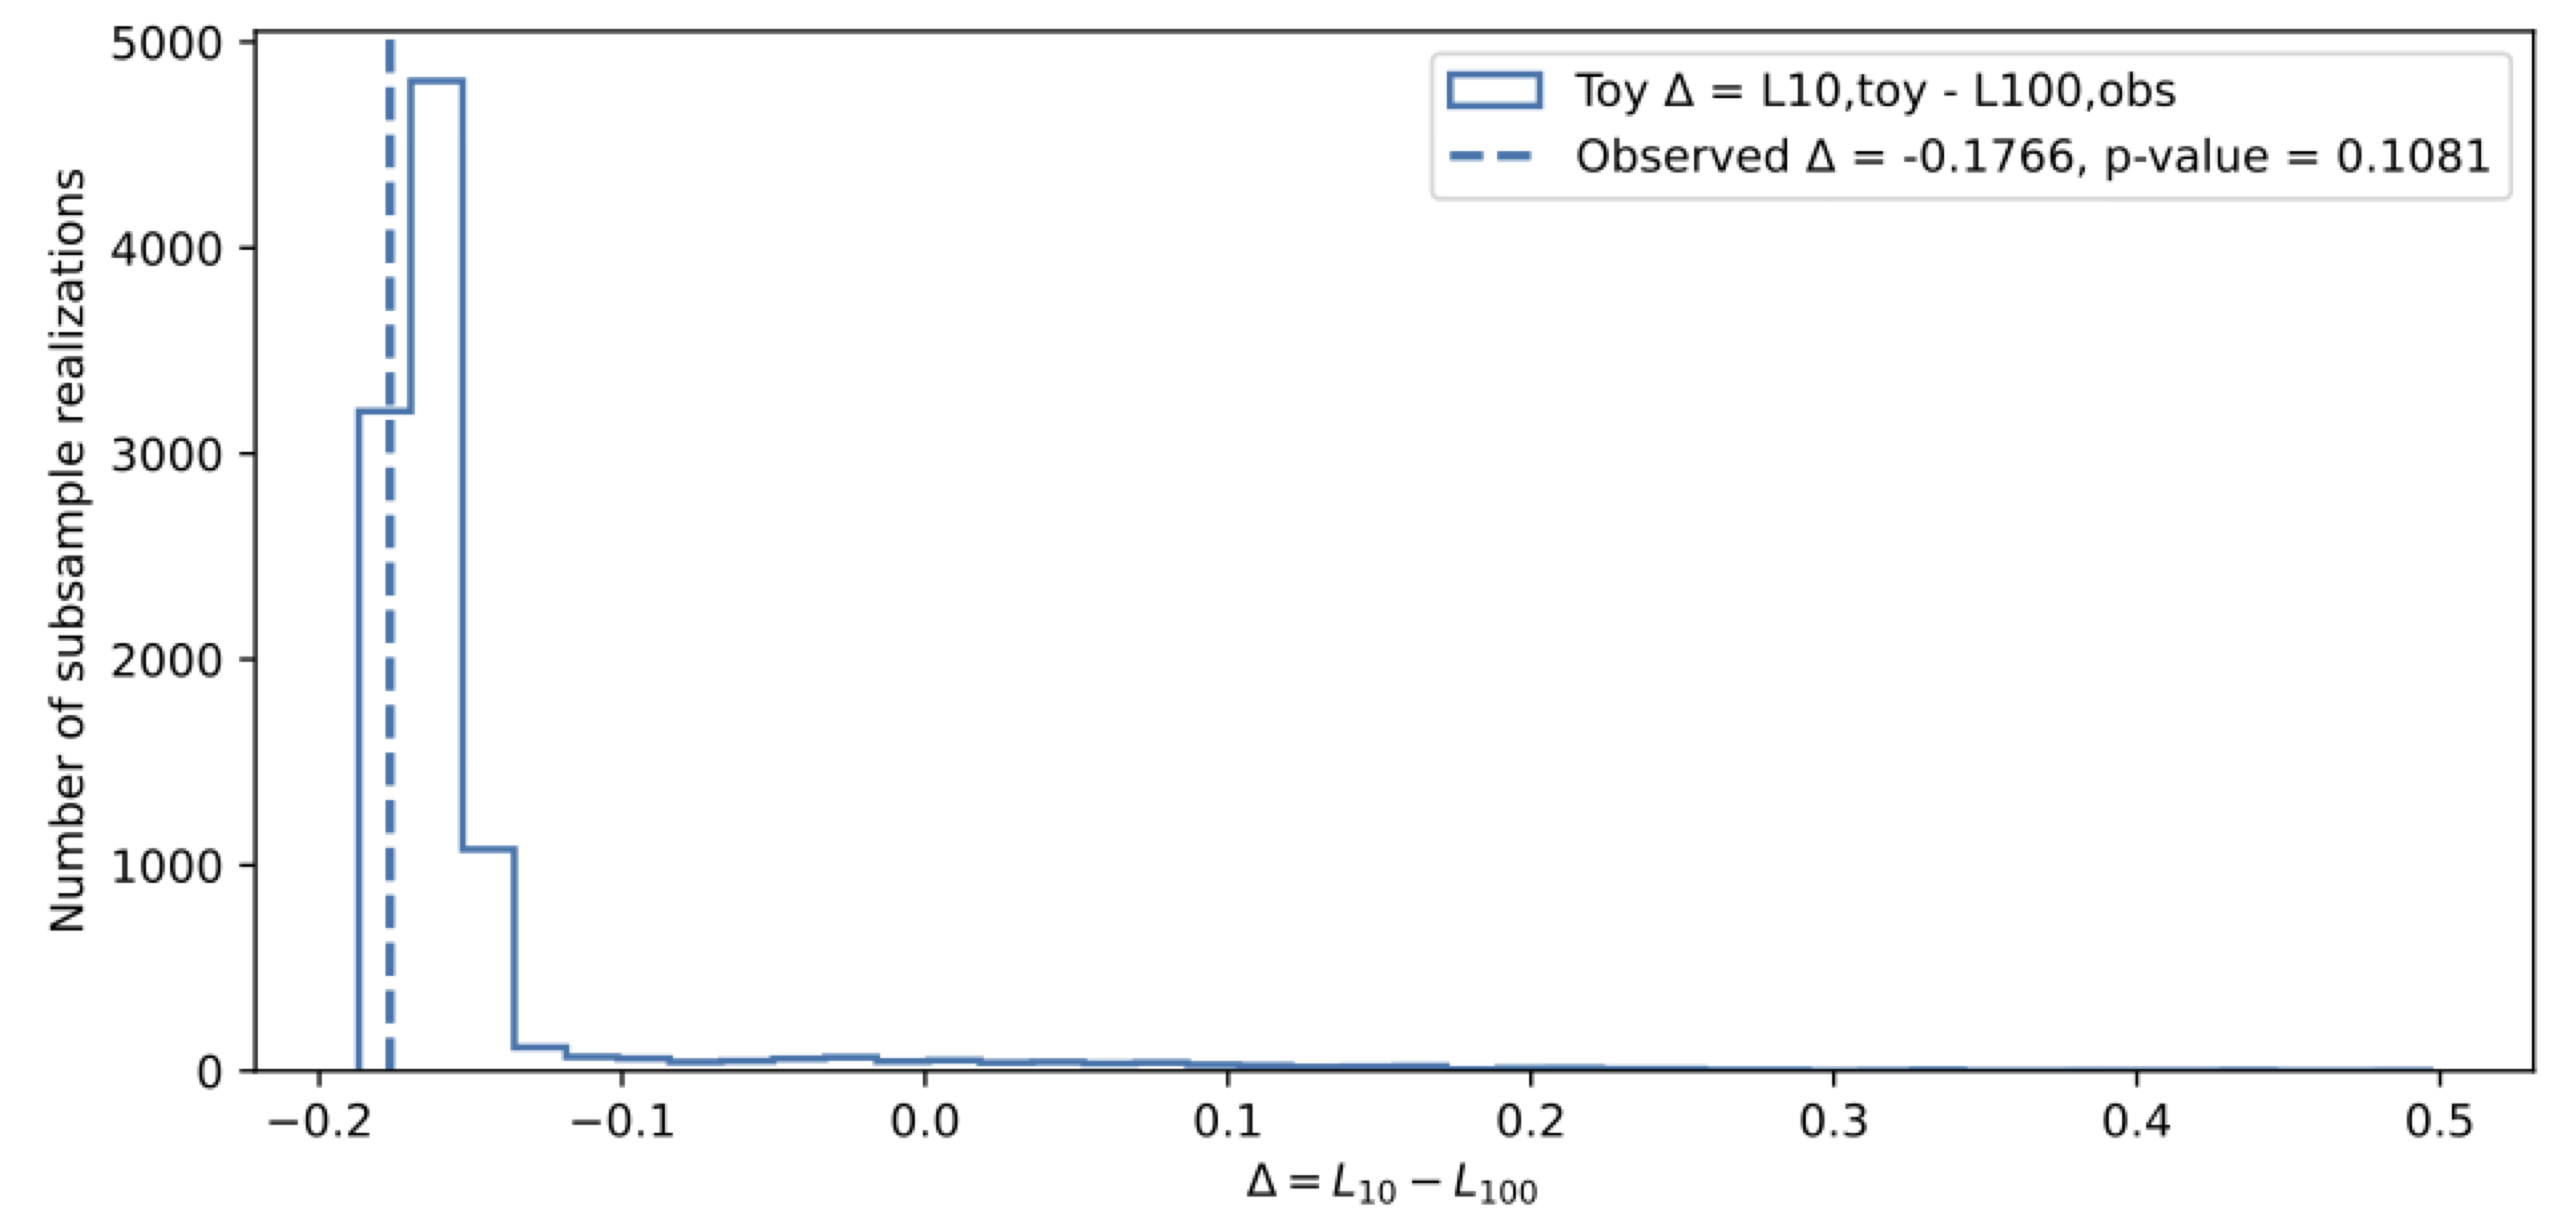
\includegraphics[
          width=\textwidth,
          alt={}
      ]{sections/5sa-analysis/images/a2_100pct_surfacecheck_toys.png}
      \caption{
        Distribution of the difference between surface background pseudoexperiments' log likelihood calculated against the model built on the 10\% and 100\% datasets (solid histogram). 
        The difference between the log likelihood of the 10\% and 100\% model compared to the observed 100\% surface background event distribution is plotted for comparison (dashed line).
      }
      \label{fig:backgroundcheck_zenith_toys}
    \end{figure}

    To quantify the agreement between the background model predicted by the 10\% sample and the one observed in the 100\% sample, we ran pseudoexperiments following a similar procedure used in Section~\ref{sec:optimization}. 
    The distribution of pseudoexperiments in relation to the observed log-likelihood with respect to the surface background model is shown in Fig.\ref{fig:backgroundcheck_zenith_toys}.
    The A2 model built on the 10\% data passed our check as the p-vale of the observed log-likelihood compared to the pseudoexperiments was greater than 0.05.
    The models for all other stations also passed this check. 

  \subsection{Thermal Background Cross Checks}

    Verifying the thermal background LDA model is performed similarly to the surface background elevation model. 
    We ensure that the thermal distribution of LDA values in the 100\% dataset is comparable to the fit made with 10\% sample via pseudoexperiments. 
    First, we plot the distribution of LDA values for thermal-like events in the 100\% data with LDA scores below the LDA cut value established in the optimization procedure defined in Section~\ref{sec:optimization}, as shown in Fig.~\ref{fig:backgroundcheck_a2c3} and Fig.~\ref{fig:backgroundcheck_a2c4} for configurations 3 and 4 of A2, respectively. 
    The pseudoexperiments are run next and if the observed log-likelihood is an outlier compared to the pseudoexperiments then the background model is assessed.
    This happened for both configurations 3 and 4 of A2 as shown in Fig.~\ref{fig:backgroundcheck_a2c3_toys} and Fig.~\ref{fig:backgroundcheck_a2c4_toys}, respectively.
    % How did we pick the outliers that we showed? 
    Results for the other stations are not discussed in this thesis but many configurations passed this thermal background check and those that did not were resolved in a similar fashion.

    \begin{figure}
      \centering
      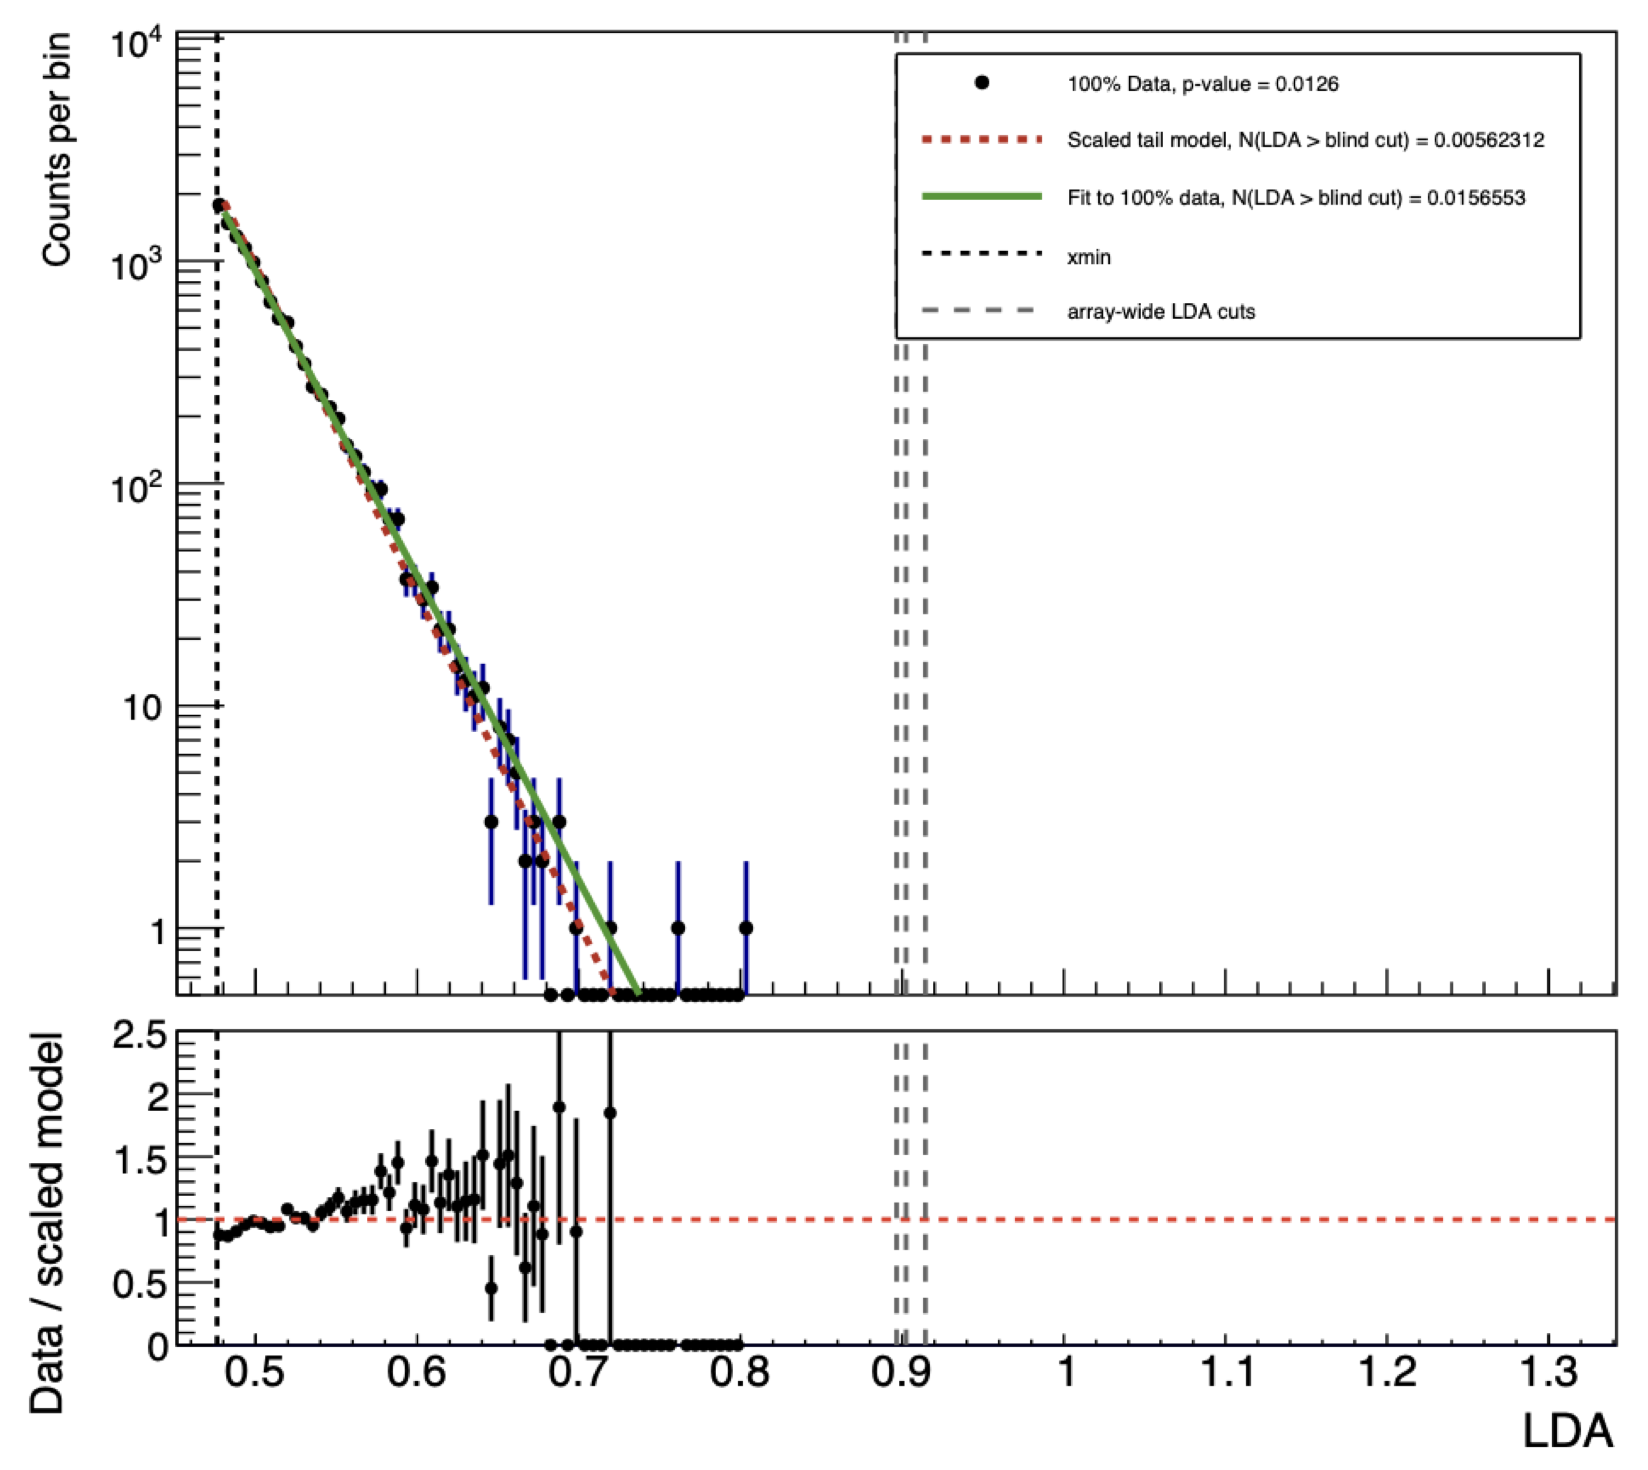
\includegraphics[
          width=0.75\textwidth,
          alt={}
      ]{sections/5sa-analysis/images/a2c3_100pct_lda_backgroundfit.png}
      \caption{
        Top: The distribution of thermal events (events that passed all cuts defined in Chapter~\ref{chap:5sa_cleaning}) from the 100\% sample of A2 configuration 3 (black dots with blue error bars).
        Only events with LDA scores greater than the $x_{\text{min}}$ used to fit the background model in Section~\ref{sec:lda} (black dotted line) and less than the appropriate LDA Cut established in Section~\ref{sec:optimization} are plotted (grey dashed lines).
        These are events are fit to an exponential (green line) plotted along the model built on the 10\% data multiplied by 10 (red dotted line).
        Bottom: Ratio of the 100\% LDA distribution of thermal events (black dots in top panel) divided by the model built on the 10\% data scaled up by a factor of 10 (red dotted line in top panel).
      }
      \label{fig:backgroundcheck_a2c3}
    \end{figure}

    \begin{figure}
      \centering
      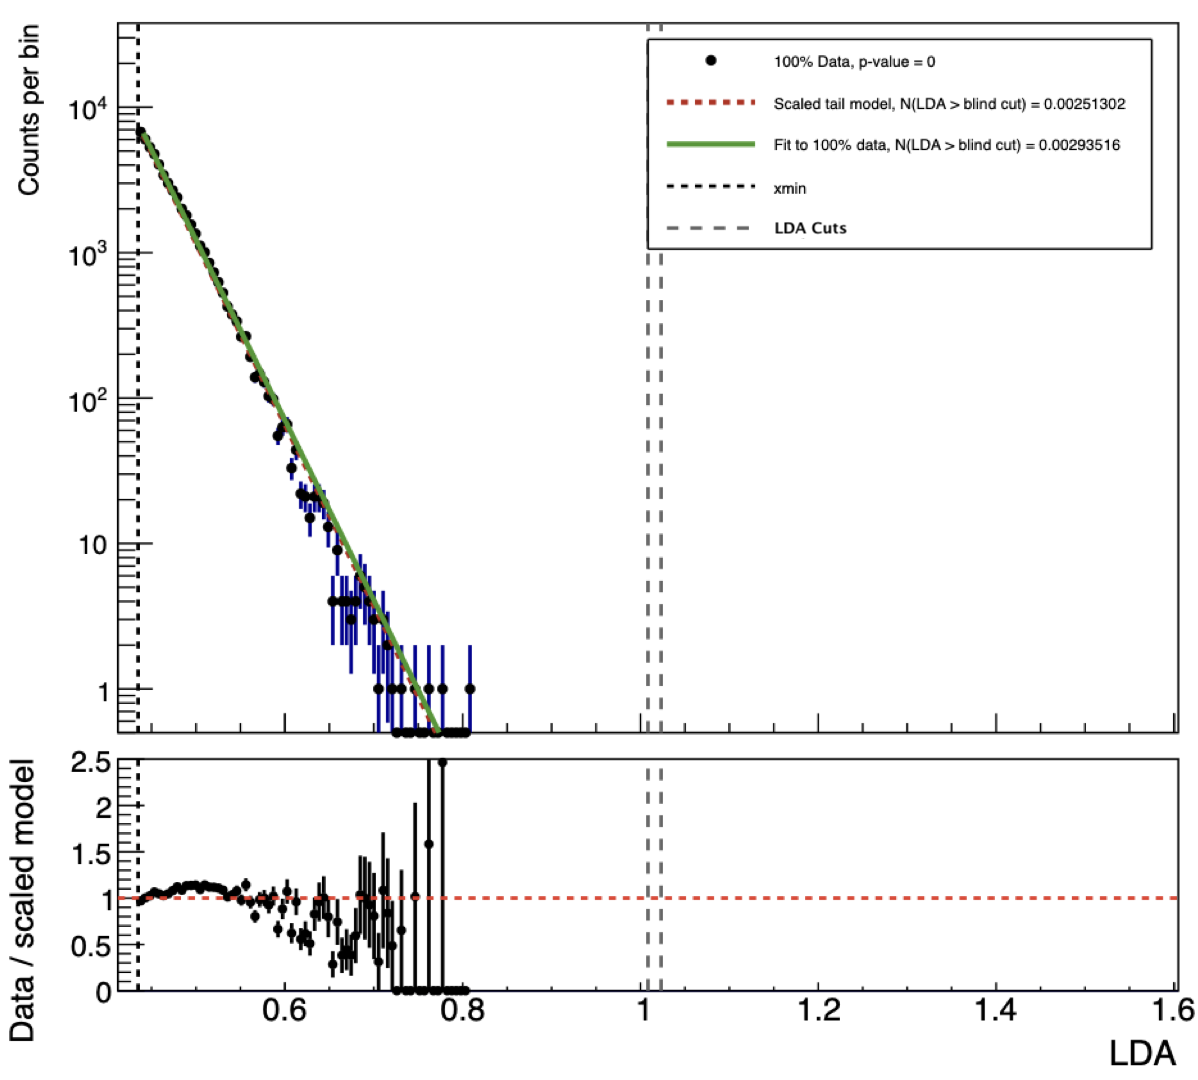
\includegraphics[
          width=0.75\textwidth,
          alt={}
      ]{sections/5sa-analysis/images/a2c4_100pct_lda_backgroundfit.png}
      \caption{
        Top: The distribution of thermal events (events that passed all cuts defined in Chapter~\ref{chap:5sa_cleaning}) from the 100\% sample of A2 configuration 4 (black dots with blue error bars).
        Only events with LDA scores greater than the $x_{\text{min}}$ used to fit the background model in Section~\ref{sec:lda} (black dotted line) and less than the appropriate LDA Cut established in Section~\ref{sec:optimization} are plotted (grey dashed lines).
        These are events are fit to an exponential (green line) plotted along the model built on the 10\% data multiplied by 10 (red dotted line).
        Bottom: Ratio of the 100\% LDA distribution of thermal events (black dots in top panel) divided by the model built on the 10\% data scaled up by a factor of 10 (red dotted line in top panel).
      }
      \label{fig:backgroundcheck_a2c4}
    \end{figure}

    \begin{figure}
      \centering
      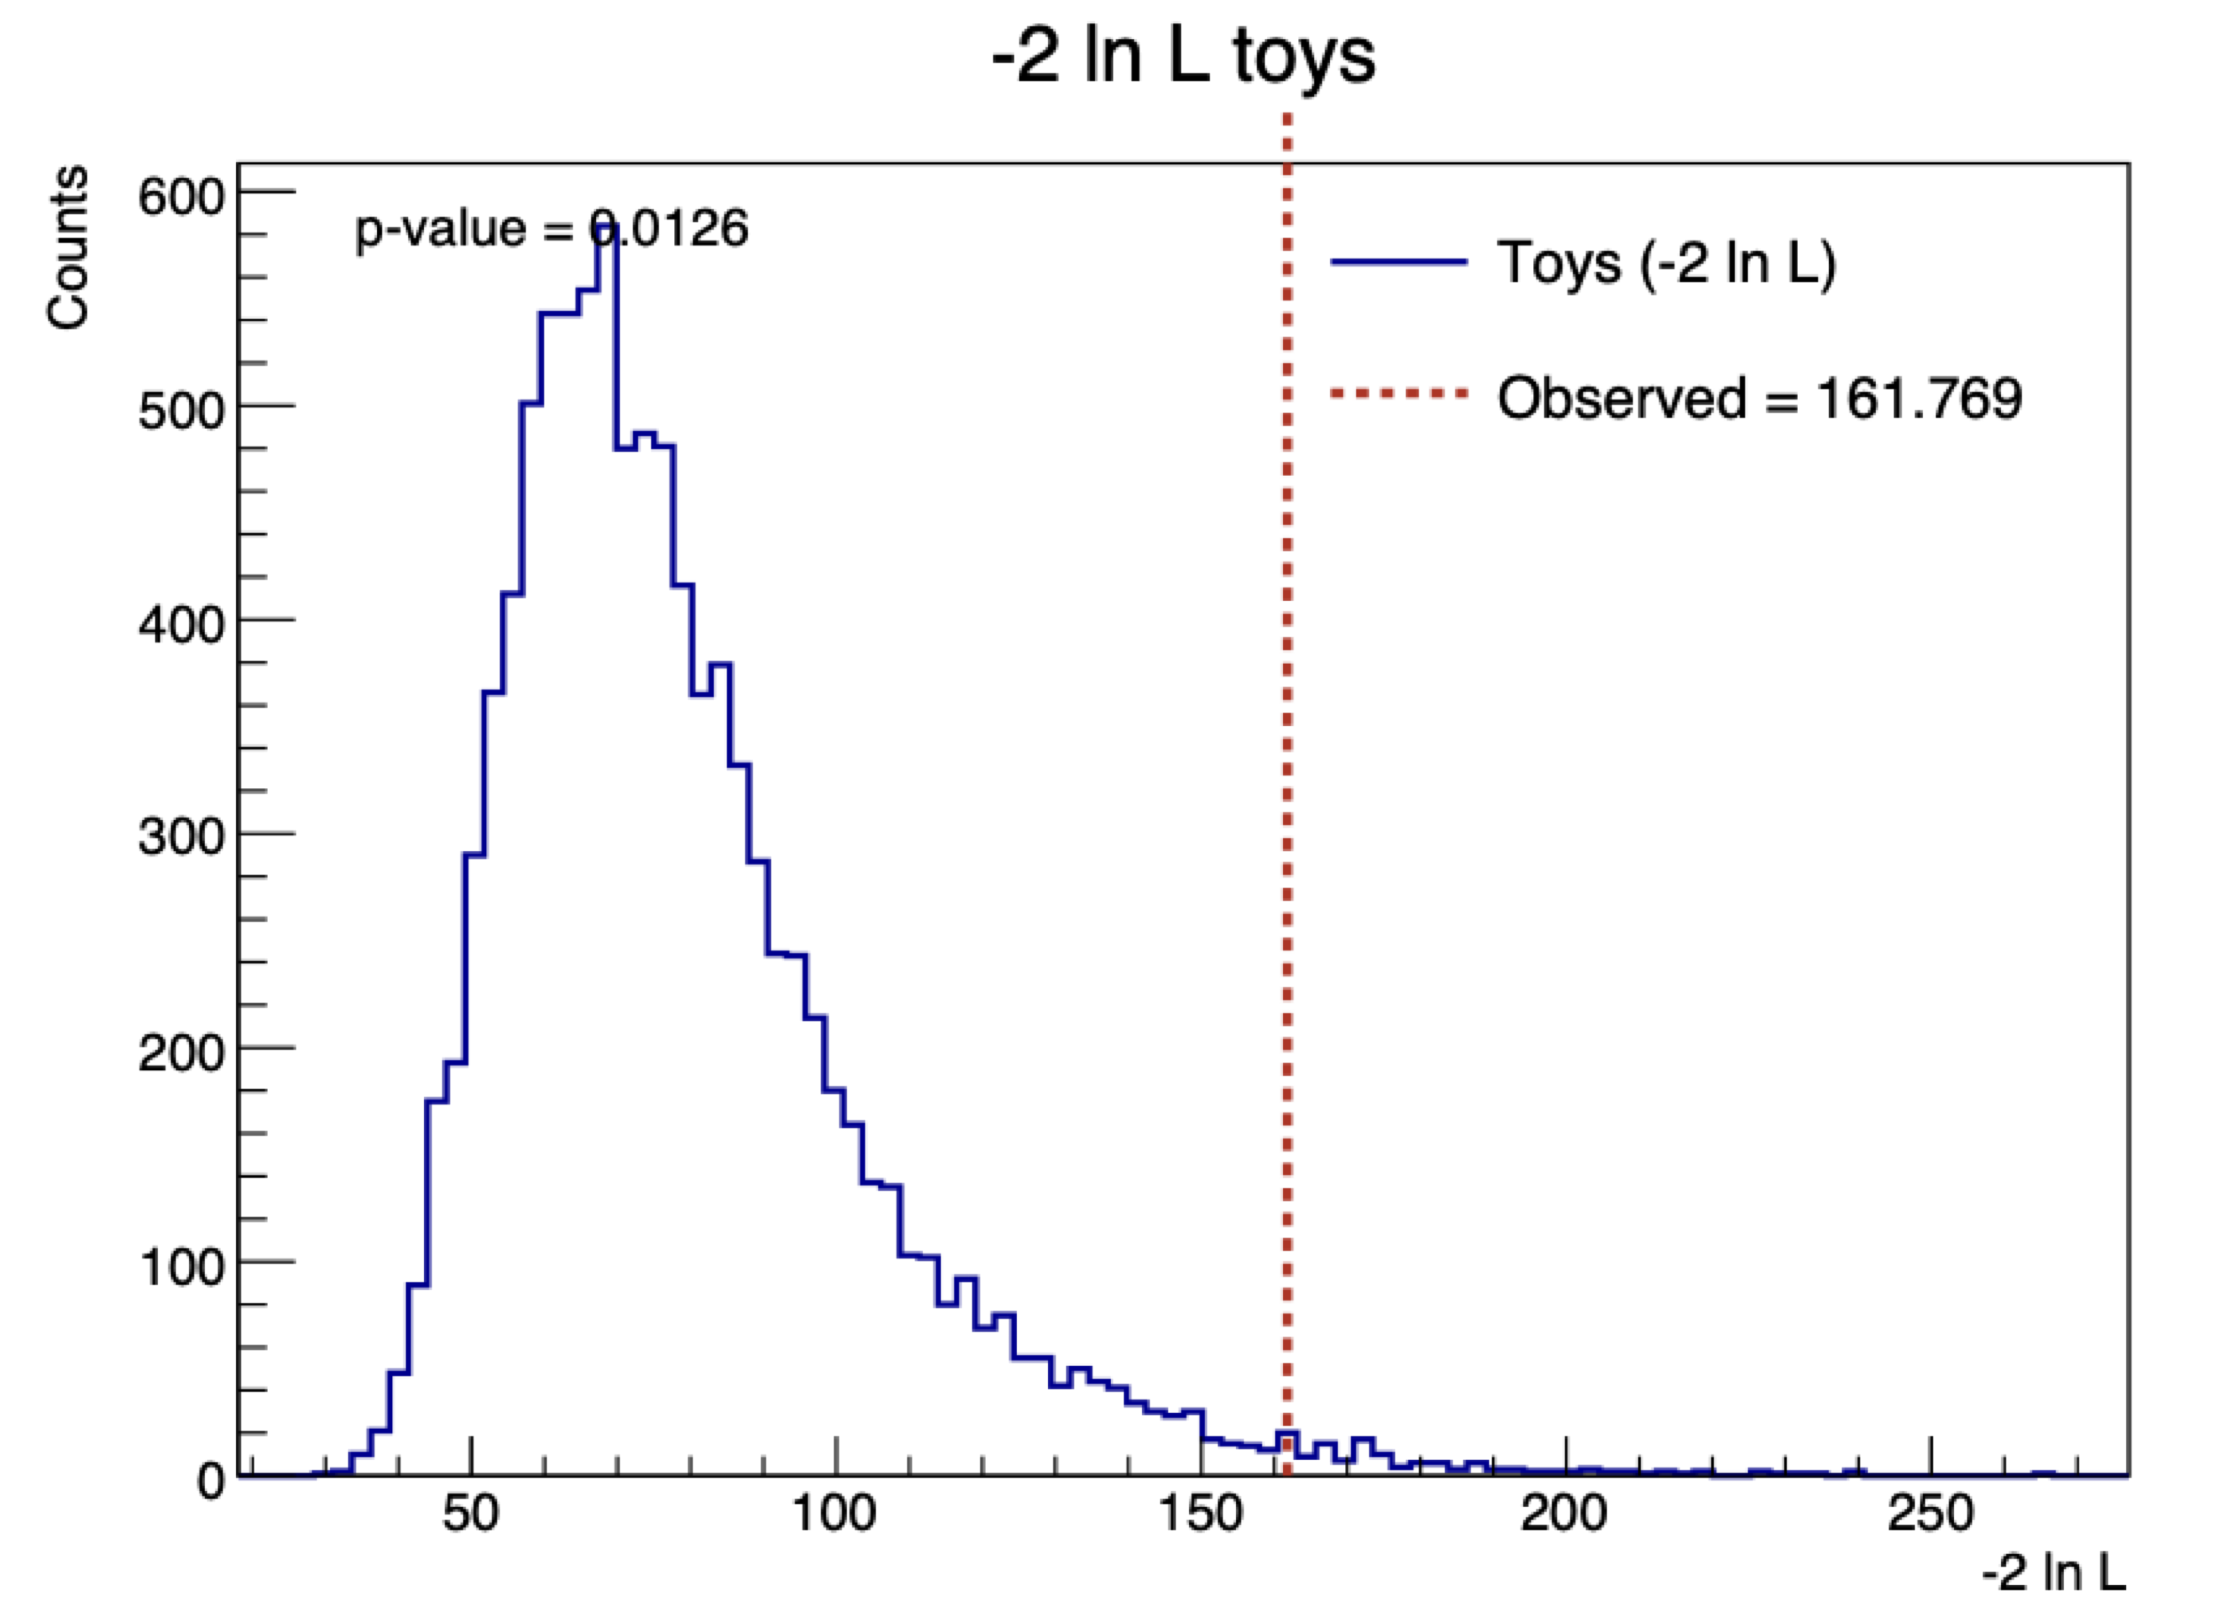
\includegraphics[
          width=0.75\textwidth,
          alt={}
      ]{sections/5sa-analysis/images/a2c3_100pct_lda_backgroundfit_toys.png}
      \caption{
        Distribution of the log-likelihood of pseudoexperiments built on 100\% A2 Configuration 3 data (blue distribution) compared to the log-likelihood of the observed 100\% data (red line) both calculated against the 10\% background model scaled up by a factor of 10.
      }
      \label{fig:backgroundcheck_a2c3_toys}
    \end{figure}

    \begin{figure}
      \centering
      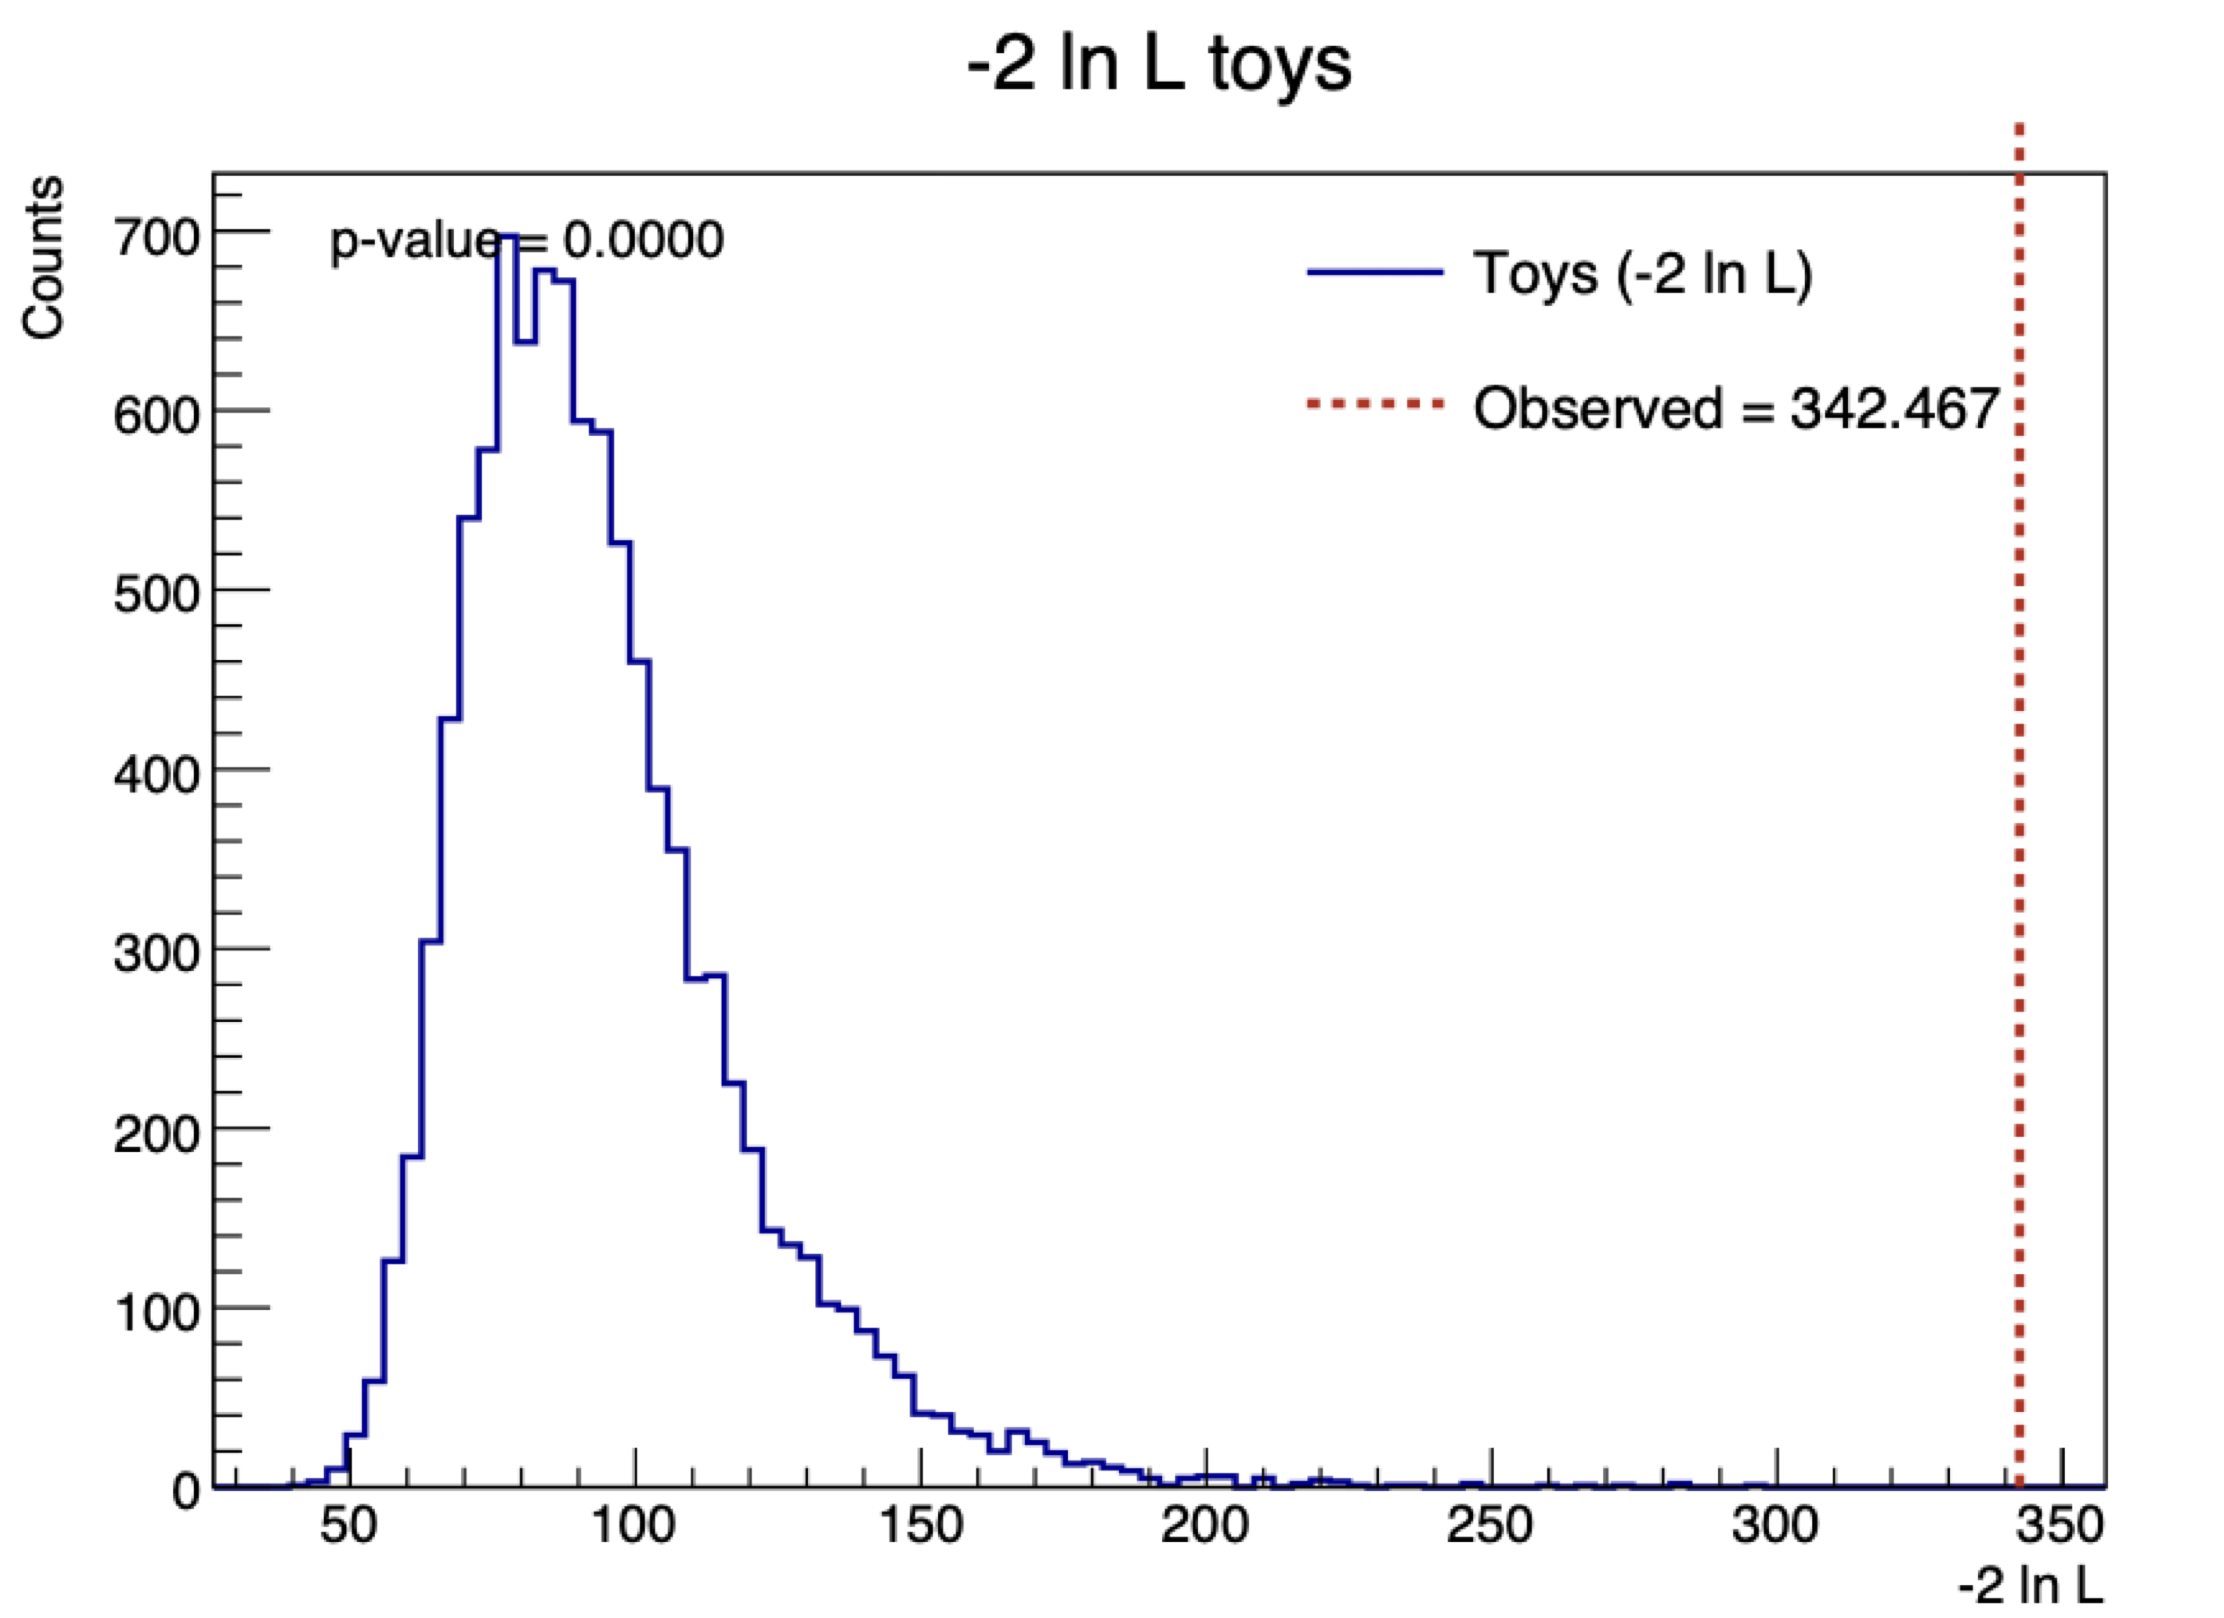
\includegraphics[
          width=0.75\textwidth,
          alt={}
      ]{sections/5sa-analysis/images/a2c4_100pct_lda_backgroundfit_toys.png}
      \caption{
        Distribution of the log-likelihood of pseudoexperiments built on 100\% A2 Configuration 4 data (blue distribution) compared to the log-likelihood of the observed 100\% data (red line) both calculated against the 10\% background model scaled up for a factor of 10.
      }
      \label{fig:backgroundcheck_a2c4_toys}
    \end{figure}

    \begin{figure}
      \centering
      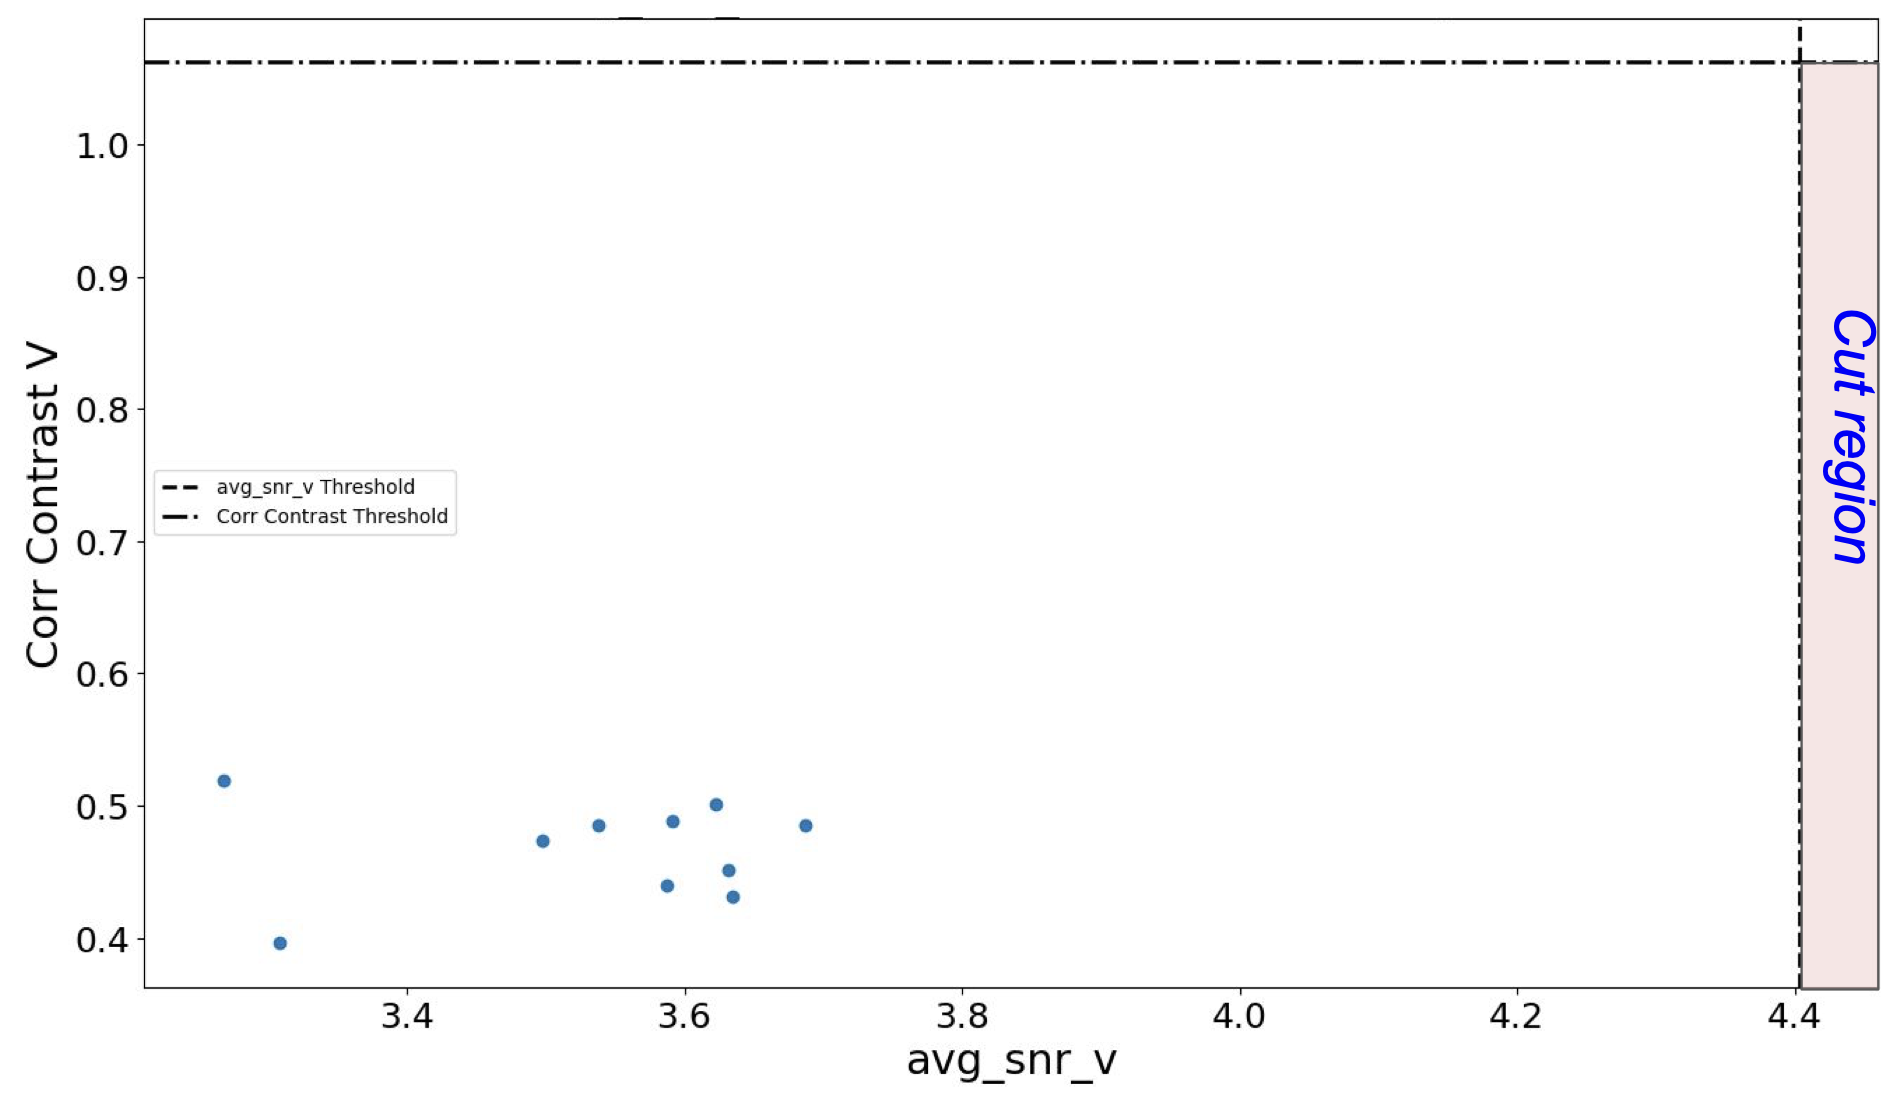
\includegraphics[
          width=0.75\textwidth,
          alt={}
      ]{sections/5sa-analysis/images/a2c3_100pct_lda_backgroundfit_outliers.png}
      \caption{
        Events from the A2 Configuration 3 distribution plotted in Fig.~\ref{fig:backgroundcheck_a2c3} with the highest LDA scores plotted by \texttt{corr\_contrast\_v} (relating the maximum reconstruction correlation score to the average) against \texttt{avg\_snr\_v} (signal strength).
        These are the variables used in the Low Reconstruction Confidence Cut defined in Section~\ref{sec:lrcc}. 
        The events plotted have \texttt{corr\_contrast\_v} well within the range the Low Reconstruction Confidence Cut isolates events for, but the \texttt{avg\_snr\_v} scores were too low for the events to be cut. 
        These events are therefore just thermal outliers with no indication that they are signal-like and would corrupt our background model.
      }
      \label{fig:backgroundcheck_a2c3_outliers}
    \end{figure}

    \begin{figure}
      \centering
      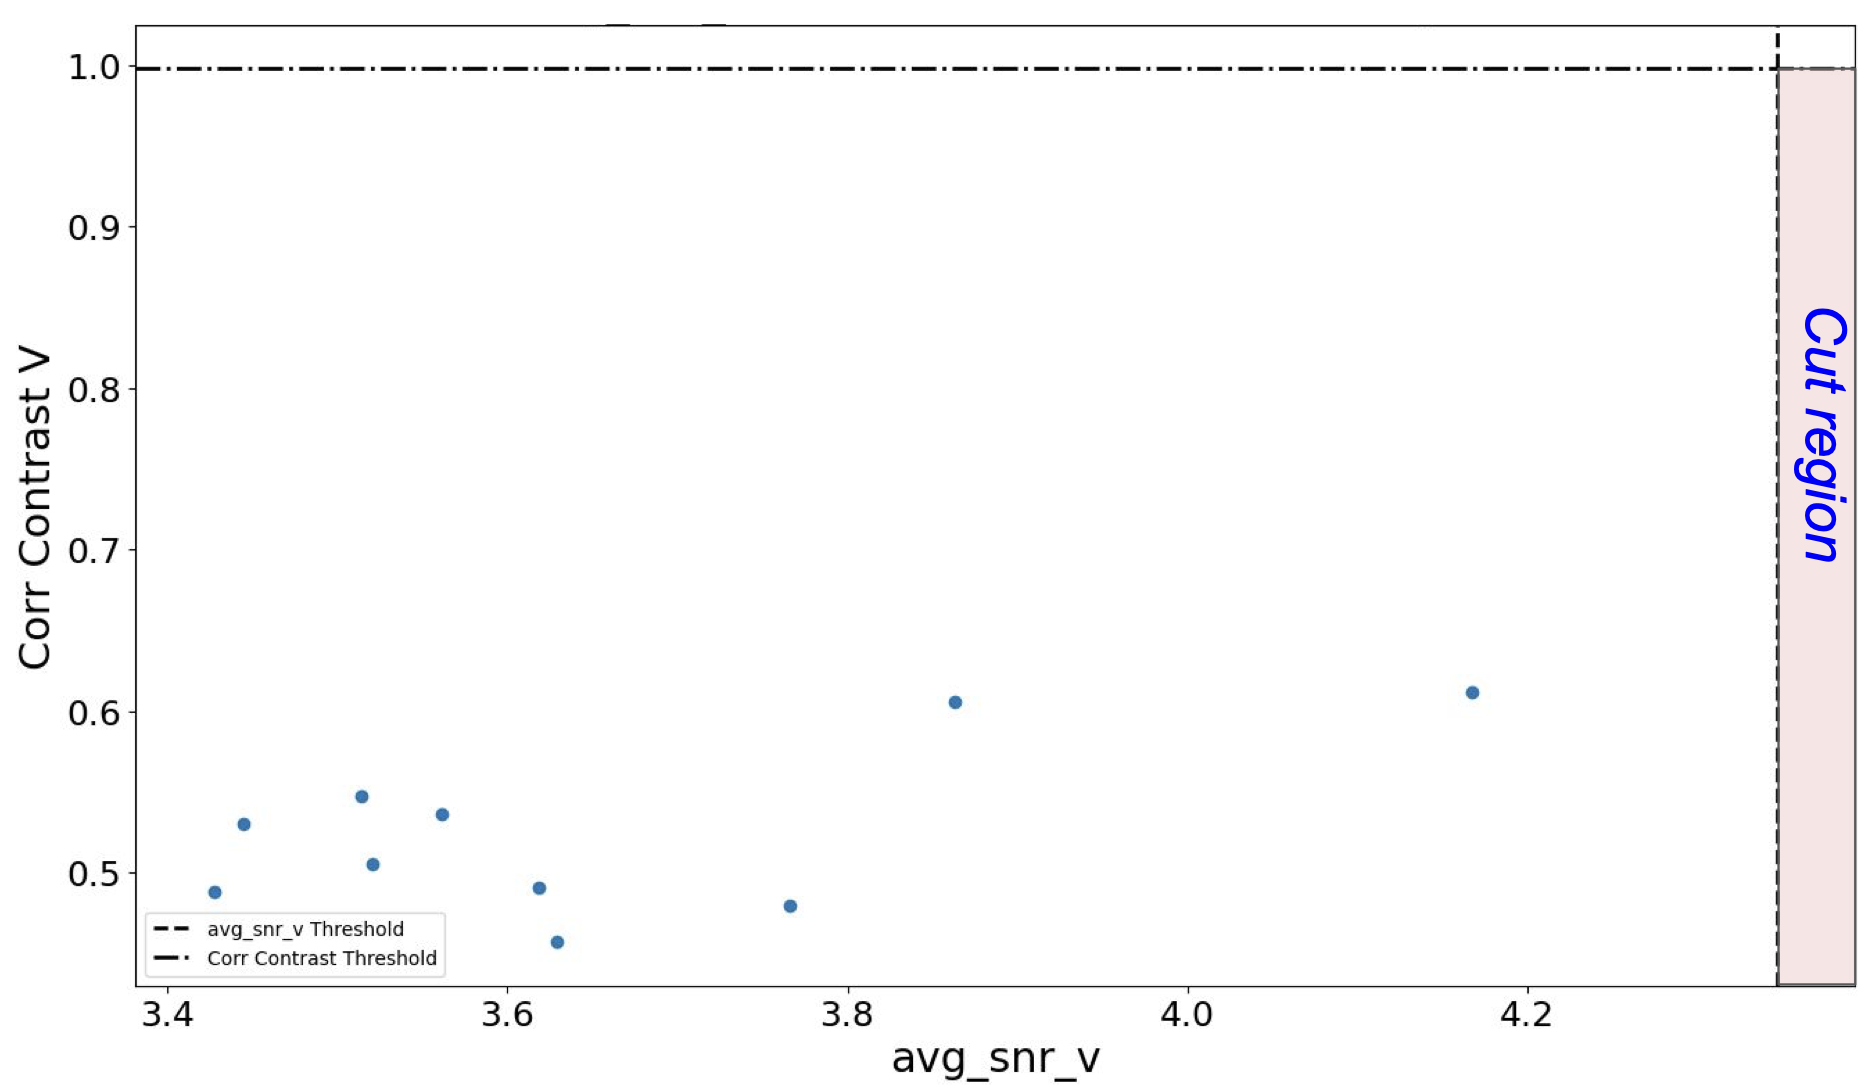
\includegraphics[
          width=0.75\textwidth,
          alt={}
      ]{sections/5sa-analysis/images/a2c4_100pct_lda_backgroundfit_outliers.png}
      \caption{
        Events from the A2 Configuration 4 distribution plotted in Fig.~\ref{fig:backgroundcheck_a2c3} with the highest LDA scores plotted by \texttt{corr\_contrast\_v} (relating the maximum reconstruction correlation score to the average) against \texttt{avg\_snr\_v} (signal strength).
        These are the variables used in the Low Reconstruction Confidence Cut defined in Section~\ref{sec:lrcc}. 
        The events plotted have \texttt{corr\_contrast\_v} well within the range the Low Reconstruction Confidence Cut isolates events for, but the \texttt{avg\_snr\_v} scores were too low for the events to be cut. 
        These events are therefore just thermal outliers with no indication that they are signal-like and would corrupt our background model.
      }
      \label{fig:backgroundcheck_a2c4_outliers}
    \end{figure}

    To investigate the low p-value on A2 configuration 3 and configuration 4, we first looked for run-level anomalies then looked at each event driving the disagreement between the 10\% model and the 100\% model.
    For configuration 3, we identified runs that had unstable firmware (6558-6569) and poor restabilization after a reported power fail (7100), all of which should have been in the Bad Run Log.
    We then established that all remaining events would have been cut by the Low Reconstruction Confidence Cut described in Section~\ref{sec:lrcc} if these events had been more signal-like, meaning these events were determined to be thermal-like but were upward fluctuations of the backgrounds enough to invalidate the background model, as shown in Fig.~\ref{fig:backgroundcheck_a2c3_outliers}.
    All outliers in the configuration 4 background LDA model were similar, they would have been removed by the Low Reconstruction Confidence Cut if they had been more signal-like, as shown in Fig.~\ref{fig:backgroundcheck_a2c4_outliers}. 
    These outliers were therefore deemed inconsequential and, after adding those runs to the Bad Run Log and therefore excluding these events from analysis, the 100\% background fit to configurations 3 and 4 were deemed to be compatible with the 10\% fits. 

  \subsection{Time Isolation Cut}

    As neutrinos are expected to be rare, it is even rarer that multiple diffuse neutrino observations would occur within a short time window. 
    To avoid collections of temporally clustered, unanticipated, neutrino-like background events from passing this analysis, we enforce a Time Isolation Cut to remove events that pass all cuts but occur within a short time window. 
    This time window was determined via a toy Monte Carlo simulation which sampled a number of neutrino events from a Poisson distribution with a mean of 15 and randomly distributed these events over the 10.6 year livetime covered by this analysis. 
    The time between consecutive events was calculated for all trials and plotted in Figure~\ref{fig:isolation_condition}.
    The time window with less than a 0.001\% probability of removing neutrinos was 5.8 hours and is used to defined the Time Isolation Cut window.

    \begin{figure}
        \centering
        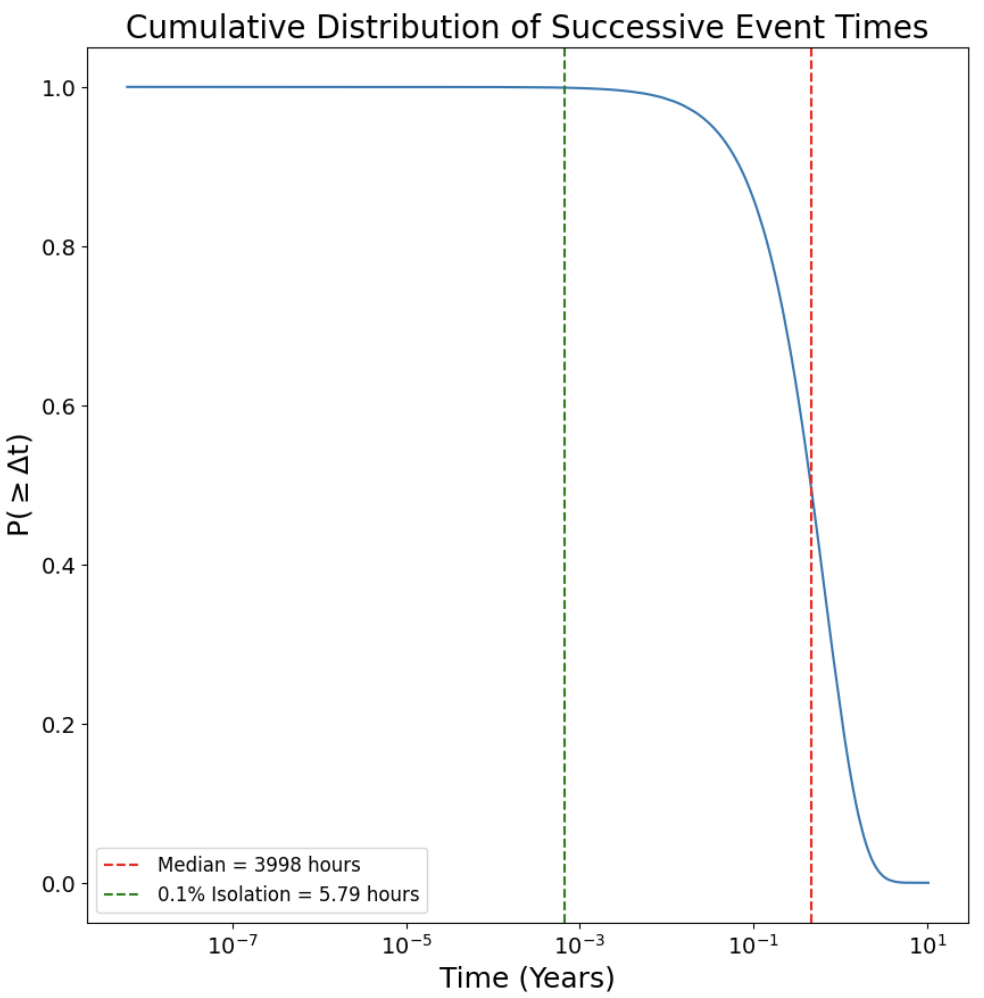
\includegraphics[
            width=0.75\textwidth,
            alt={}
        ]{sections/5sa-analysis/images/isolation.png}
        \caption{
          Cumulative distribution of the time difference between successive events in the toy Monte Carlo simulation of neutrino event detection times (blue).
          The average time separation between successive neutrino events is 3998 hours (red, 5.48 months).
          99.9\% of events occur at least 5.79 hours apart (green).
        }
        \label{fig:isolation_condition}
    \end{figure}

    However, this analysis considers neutrino events that may involve multiple cascades resulting from muon stochastic losses, tau stochastic losses, and tau decays. 
    We expect that these types of events will not trigger the same detector twice very often, given the lengthy, $\mathcal{O}(\text{1 ms})$ deadtime of ARA stations and geometric constraints of Askaryan radiation, but in Figure~\ref{fig:multistation} we showed that we expect multiple stations to observe one or more cascades resulting from $10^{19}$~eV neutrinos 10\% of the time, increasing to 35\% for neutrinos with $10^{21}$~eV of energy.
    We therefore retain passing event multiplets within a time window of 5~s. 

\pagebreak
\section{Inspection of Passing Events \label{sec:passing_events}}

    As this type of experiment and analysis expects to observe 0 or 1 event on a background of $\sim\!0$ events, any events that pass all analysis cuts will need to be assessed to determine if they are consistent with simulated neutrino events or some unanticipated technical background. 
    The analysis will not be substantially changed, however a posteriori inspection of any new backgrounds may warrant an update to the analysis cuts. 
    This should be performed in a regimented way and cuts should only be made more conservative.

    \subsection{Approach to Analyzing Unblinded Data}

      For any events that pass all analysis cuts, our goal is to analyze all analysis variables for the events before consulting the waveform and reconstruction skymap - preserving analysis ``blindness'' as long as possible. 
      Some examples of first stage analyzes include analyzing the time each event occurred, the reconstructed azimuth and elevation of events, conducting a KS test for azimuthal randomness, and consulting analysis variables associated with the Spark Event Cut and Anomalous Channel Cut which identify glitches. 
      If more information is needed, we will then consult the event waveforms, spectra, and reconstruction skymaps. 
      We expect that the only events that pass the analysis will be neutrino candidates.
      If a population of events passes the analysis and is subsequently determined to be inconsistent with our expectation of neutrino observations, appears to be a new class of unanticipated glitches or unexpected technical background, and can be removed in a principled fashion, then we will employ a new cut and the events will not be included in the upcoming Feldman Cousins factor calculation that determines the upper limit set by the analysis. 
      Any remaining events will be assessed for compatibility with our expectation of neutrino observations. % How is this different from an LDA? why didn't we use this instead of the LDA?
      If any events are more consistent with background than expected neutrino events, we will update our background estimate if the Poisson p-value to observe such an upward fluctuation is greater than $3\sigma$.

      Ultimately, the number of events that pass this analysis and that cannot be explained as an unanticipated background will contribute to the number of observed neutrino candidates by this analysis.
      This will be used to calculate the neutrino flux or upper limit on the neutrino flux in Section~\ref{sec:5sa_results}.

    \subsection{A Posterior Investigation of the Passing Event}

      The results of the analysis on the 100\% revealed a single passing event taken by the Phased Array (PA). 
      As only one event was found, no events were cut by the Time Isolation Cut. 
      After analyzing the event, we determined that it was a glitch.
      Furthermore, we identified that this class of events is a type of technical background that has been observed on stations A1-A5.
      Two dedicated cuts were already developed and used to address this class of events, the Spark Event Cut and the Anomalous Channel Cut.
      Earlier investigations assumed the malfunction was on the data acquisition (DAQ) board of A1-A5 which would not affect the PA which has a different DAQ board.
      However, closer inspection of this event indicated downhole electronics emitted radiation.
      This causes the waveforms of some channels to saturate while simultaneously generating radio-wavelength emission that is observed by nearby antennas.
      This means that glitches on A5 strings can be observed by the PA.
      We have not seen this glitch occur on the PA string.
      Given this new understanding, we expanded the cuts to remove PA events within 0.1~s of A5 events removed by the Spark Event Cut and the Anomalous Event Cut. 
      This removes the passing event so it will not be included in the Feldman Cousins upper limit calculation.
      The rest of this section details the study of this event following the prescription outlined in the previous section and how we determined this event was caused by a glitch. 

      \begin{figure}
        \centering
        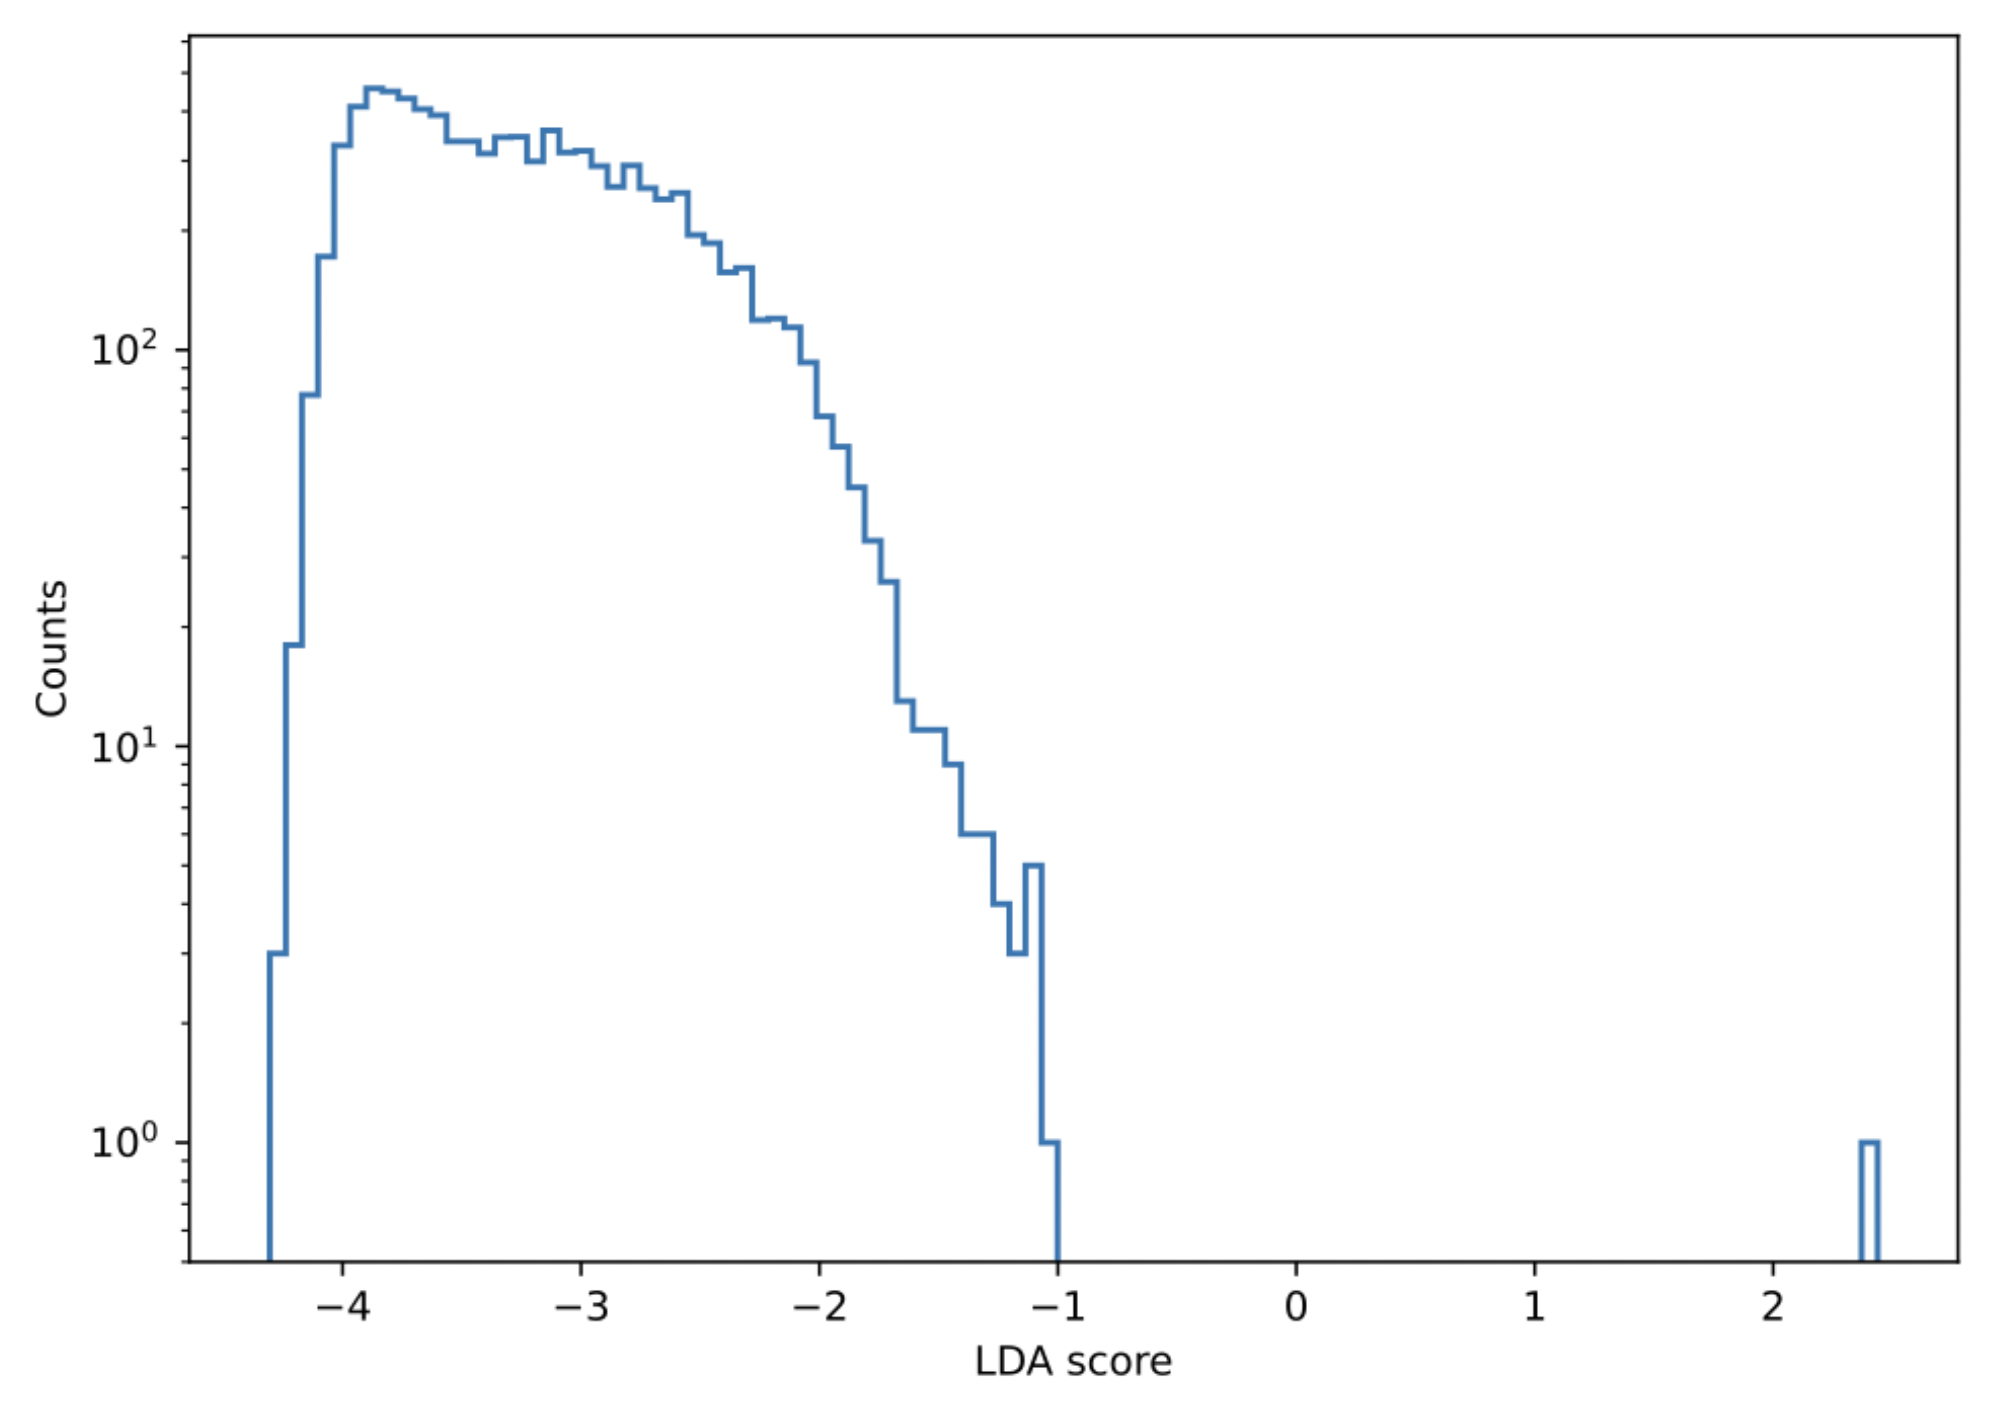
\includegraphics[
          width=0.7\linewidth,
          alt={}
        ]{sections/5sa-analysis/images/passing_lda_parun767.png}
        \caption{
          LDA distribution of events in PA run 767. The event that passed the analysis is the outlier with an LDA score of 2.43 and the LDA cut for this configuration was 1.17.
        }
        \label{fig:passing_LDA}
      \end{figure}

      The passing event's LDA score was 2.43 and was a significant outlier to the rest of the events in the run, as shown in Figure~\ref{fig:passing_LDA}.
      Some analysis variables of the PA event are presented in Table~\ref{tab:paevent} but the full suite is provided in Appendix~\ref{app:pa_passingevent}. 
      In short, this event
      \begin{itemize}
        \item was taken on April 4, 2018 at 06:01:17 UTC,
        \item saturated the PA DAQ when it was recorded,
        \item observed an SNR of 12.5 in the VPols, and
        \item observed an SNR of 11.8 in the HPols.
      \end{itemize}
      The event reconstructs to an elevation of $-35^{\circ}$ and, from the \texttt{mindepth\_v}, indicates that the highest elevation with a reconstruction correlation score that is 60\% of the maximum lies at an elevation angle of $-27.6^{\circ}$.
      This reconstruction is of good quality and suggests an in-ice origin for this signal.

      \begin{table}
        \centering
        \begin{tabular}{
          | >{\centering\arraybackslash}m{3.5cm}  
          | >{\centering\arraybackslash}m{3.5cm}  
          | >{\centering\arraybackslash}m{2.5cm}  
          >{\centering\arraybackslash}m{3.5cm}  |
        }
          \hline
          PA Analysis Variable & Corresponding AraProc Analysis Variable & Value & Note \\
          \hline
          \texttt{avgHpolSnr} & \texttt{avg\_snr\_h} & 11.78 &  \\
          \texttt{avgPaSnr} & \texttt{avg\_snr\_v} & 12.46 &  \\
          \texttt{avgRms} & \texttt{avg\_rms\_v} & 57.71 V &  \\
          \texttt{bestCorr} & \texttt{global\_max\_corr} & 0.18 &  \\
          \texttt{bestPhi} & \texttt{global\_max\_phi} & 5.67 rad &  \\
          \texttt{bestTheta} & \texttt{global\_max\_theta} & 2.18 rad & Elevation angle \\
          \texttt{corrContrast} & \texttt{corr\_contrast\_v} & 7.01 &  \\
          \texttt{cswPaSnr} & \texttt{csw\_snr\_v} & 12.89 &  \\
          \texttt{eventNo} & \texttt{event\_number} & 89985 &  \\
          \texttt{imp} & \texttt{impulsivity\_v} & 0.81 &  \\
          \texttt{ldaScore} & \texttt{} & 2.44 &  \\
          \texttt{runNo} & \texttt{run\_number} & 767 &  \\
          \texttt{s2} & \texttt{avg\_s2\_v} & 11.25 &  \\
          \texttt{unixTime} & \texttt{unixtime} & 1522821677 &  \\
          \hline
        \end{tabular}
        \caption{
          Analysis variables for the passing event calculated using the PA analysis framework, the corresponding analysis variable calculated by AraProc, the value of the PA analysis variable, and any notes regarding the variable.
        }
        \label{tab:paevent}
      \end{table}

      \begin{figure}
        \centering
        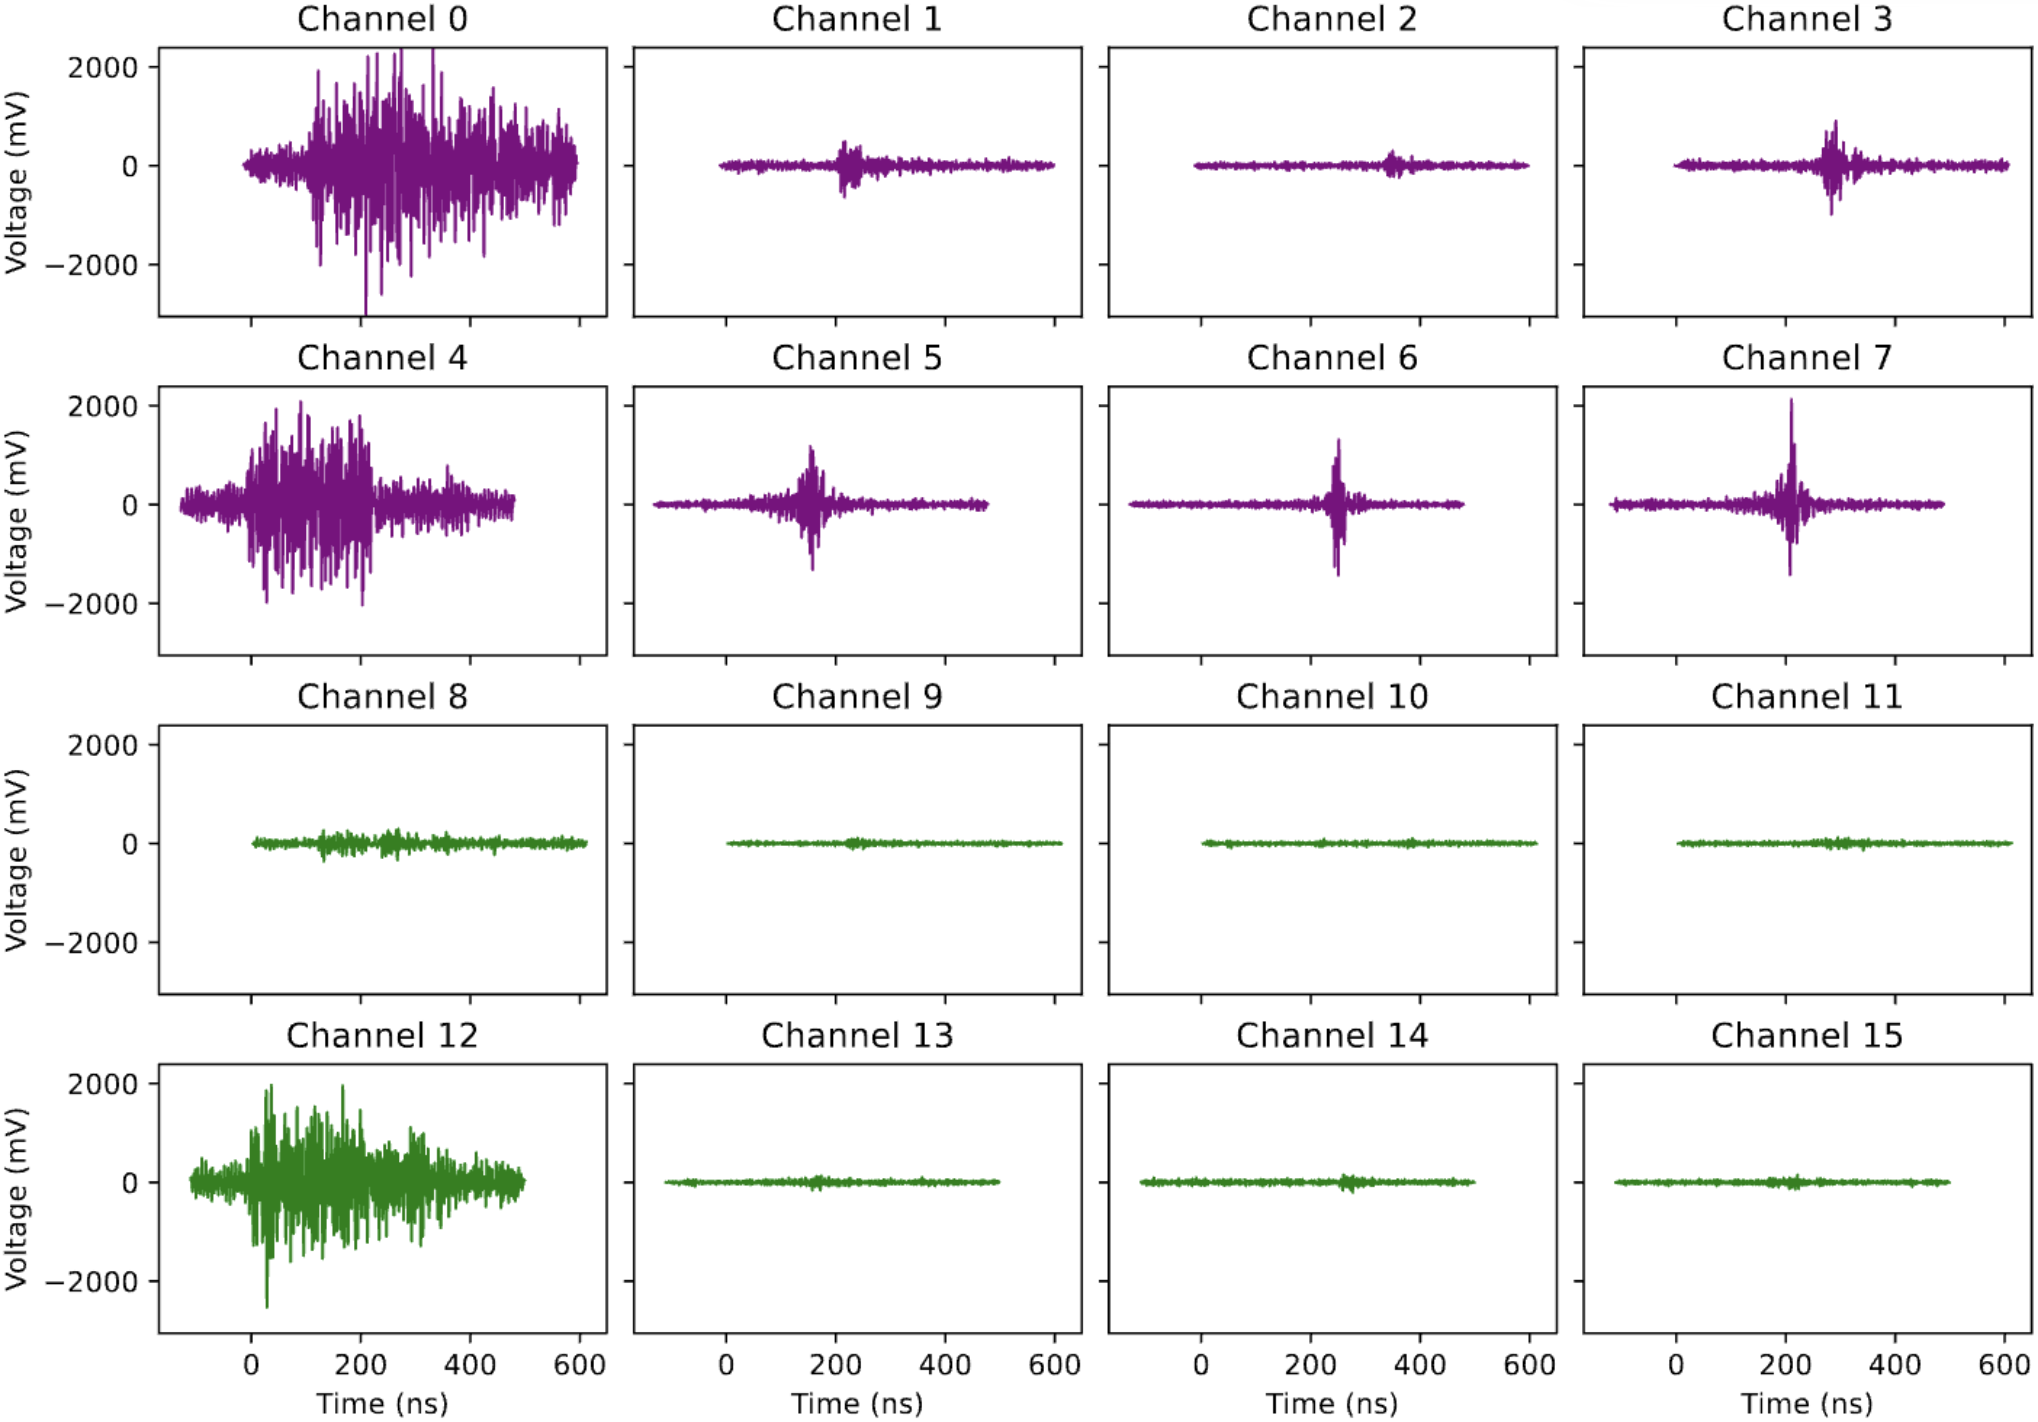
\includegraphics[
          width=\linewidth,
          alt={}
        ]{sections/5sa-analysis/images/passingevent_a5waveform.png}
        \caption{
          The voltage versus time waveforms in each A5 antenna for event 64066 of Run 2899, the A5 event corresponding to the PA event that passed the analysis.
          The high root-mean-square voltage observed in Channel 0, 4, and 12 (which are all located on the same string) is a typical feature of the events removed by the Anomalous Channel Cut defined in Section~\ref{sec:acc}.
          Impulsive signals are also visible on the three other A5 strings.
        }
        \label{fig:passing_a5waveform}
      \end{figure}

      The PA is colocated with A5 and an A5 event was recorded at the same time as this passing PA event.
      % As discussed in Section~\ref{sec:triggering}, signals that trigger both A5 and the PA trigger A5 first
      The A5 event was removed from the analysis by the Anomalous Channel Cut and indicate anomalous waveforms incompatible with expectations of a neutrino observation.
      Figure~\ref{fig:passing_a5waveform} shows high root-mean-square voltage in channels 0, 4, and 12 and impulsive signatures on strings 2, 3 and 4 of the A5 event. 
      The characteristics of these waveforms are consistent with the A4 event that inspired the Anomalous Channel Cut\index{Cut, Anomalous Channel} as described in Section~\ref{sec:acc}.

      We also looked for events in stations A1-A4 that occurred within 24 hours of the passing PA event. 
      We found no events in A1-A3 and one event in A4 that occurred within 0.5~seconds of the PA and A5 events. 
      This A4 event was also the same event from the 10\% sample that motivated the creation of the Anomalous Channel cut. 
      The A4 event is shown in Figure~\ref{fig:a4outlier} demonstrating the same waveform characteristics as the A5 event shown in Figure~\ref{fig:passing_a5waveform}- one string has multiple antenna waveforms demonstrating power surges and impulsive signatures on the remaining strings.
      There were no activities or occurrences that could explain the A4, A5, and PA events with our current understanding, including ARA monitoring activities, IceCube activities, activation of the radio pulsers at the top of the IceCube volume, South Pole Station activities, and natural phenomena (e.g. earthquakes, solar activity, etc)

      % Our list was as follows: 
      % \begin{itemize}
      %   \item Do all waveforms have a pulse?
      %   \item Do the spectra resemble Askaryan radiation?
      %   \item Are all waveforms similar?
      %   \item Do any channels have waveforms similar to channels 0, 4, 12 in the coincident A5 event shown in Fig.~\ref{fig:passing_a5waveform}?
      % \end{itemize}
      The waveform for the PA passing event is shown in Fig.~\ref{fig:passing_pawaveform}. 
      Immediately, we see that each waveform has a clear pulse, they all look similar, and none resemble channels 0, 4, and 12 in the A5 passing event.
      The PA waveforms all look similar to the waveforms observed by A5 strings 2, 3, and 4 - resembling calibration pulsers, like the one shown in Figure~\ref{fig:noiseevent}. 
      However, the A5 event does not reconstruct into the region where calibration pulsers lie.

      \begin{figure}
        \centering
        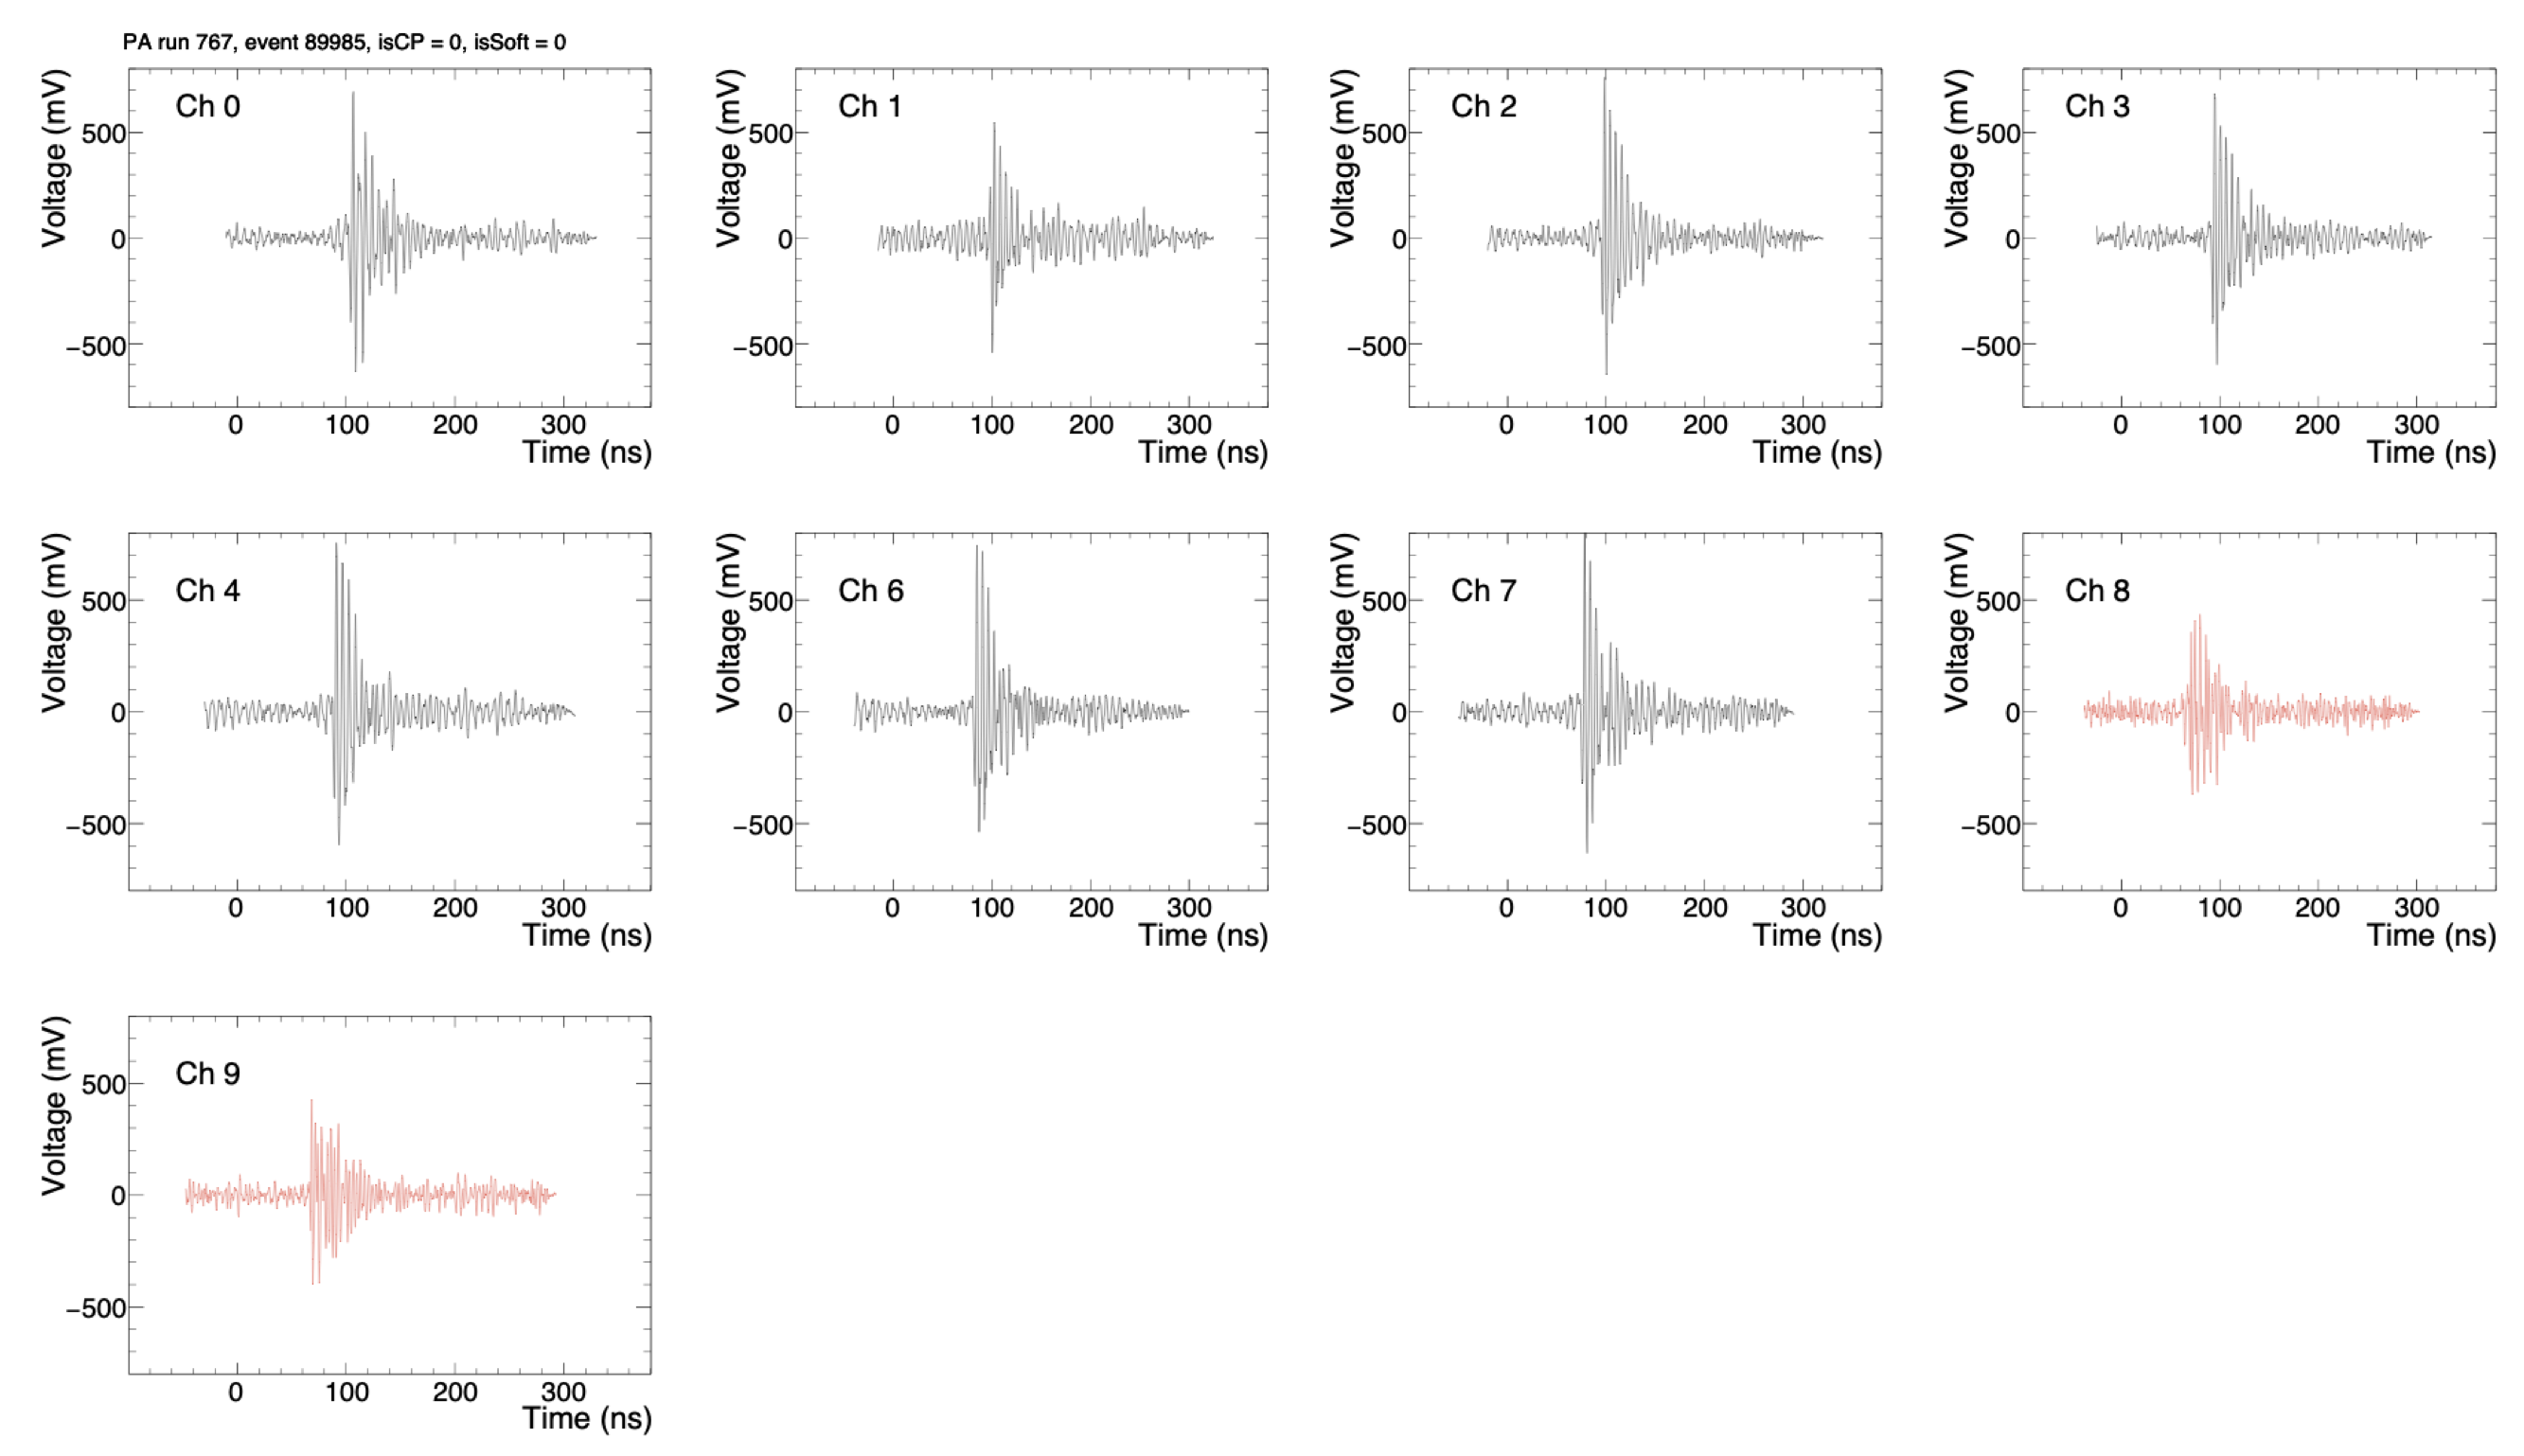
\includegraphics[
          width=\linewidth,
          alt={}
        ]{sections/5sa-analysis/images/passing_pawaveform.png}
        \caption{
          The voltage versus time waveforms in each PA antenna for event 89985 of Run 767, the event that passed the analysis.
          Channel 0 is the top antenna of the PA string and channel 9 is the bottom antenna.
          Channels 0-7 (black) are the vertically polarized antennas from which we construct the PA trigger. 
          Channel 8 and channel 9 (red) are the horizontally polarized antennas at the bottom of the PA string used to enhance angular event reconstruction.
          % This is bandpassed
        }
        \label{fig:passing_pawaveform}
      \end{figure}

      % \comment{I could show the PA event's spectrum and compare it to a calibration pulser but I'd need to ask Marco to generate it for me.}

      \begin{figure}
        \centering
        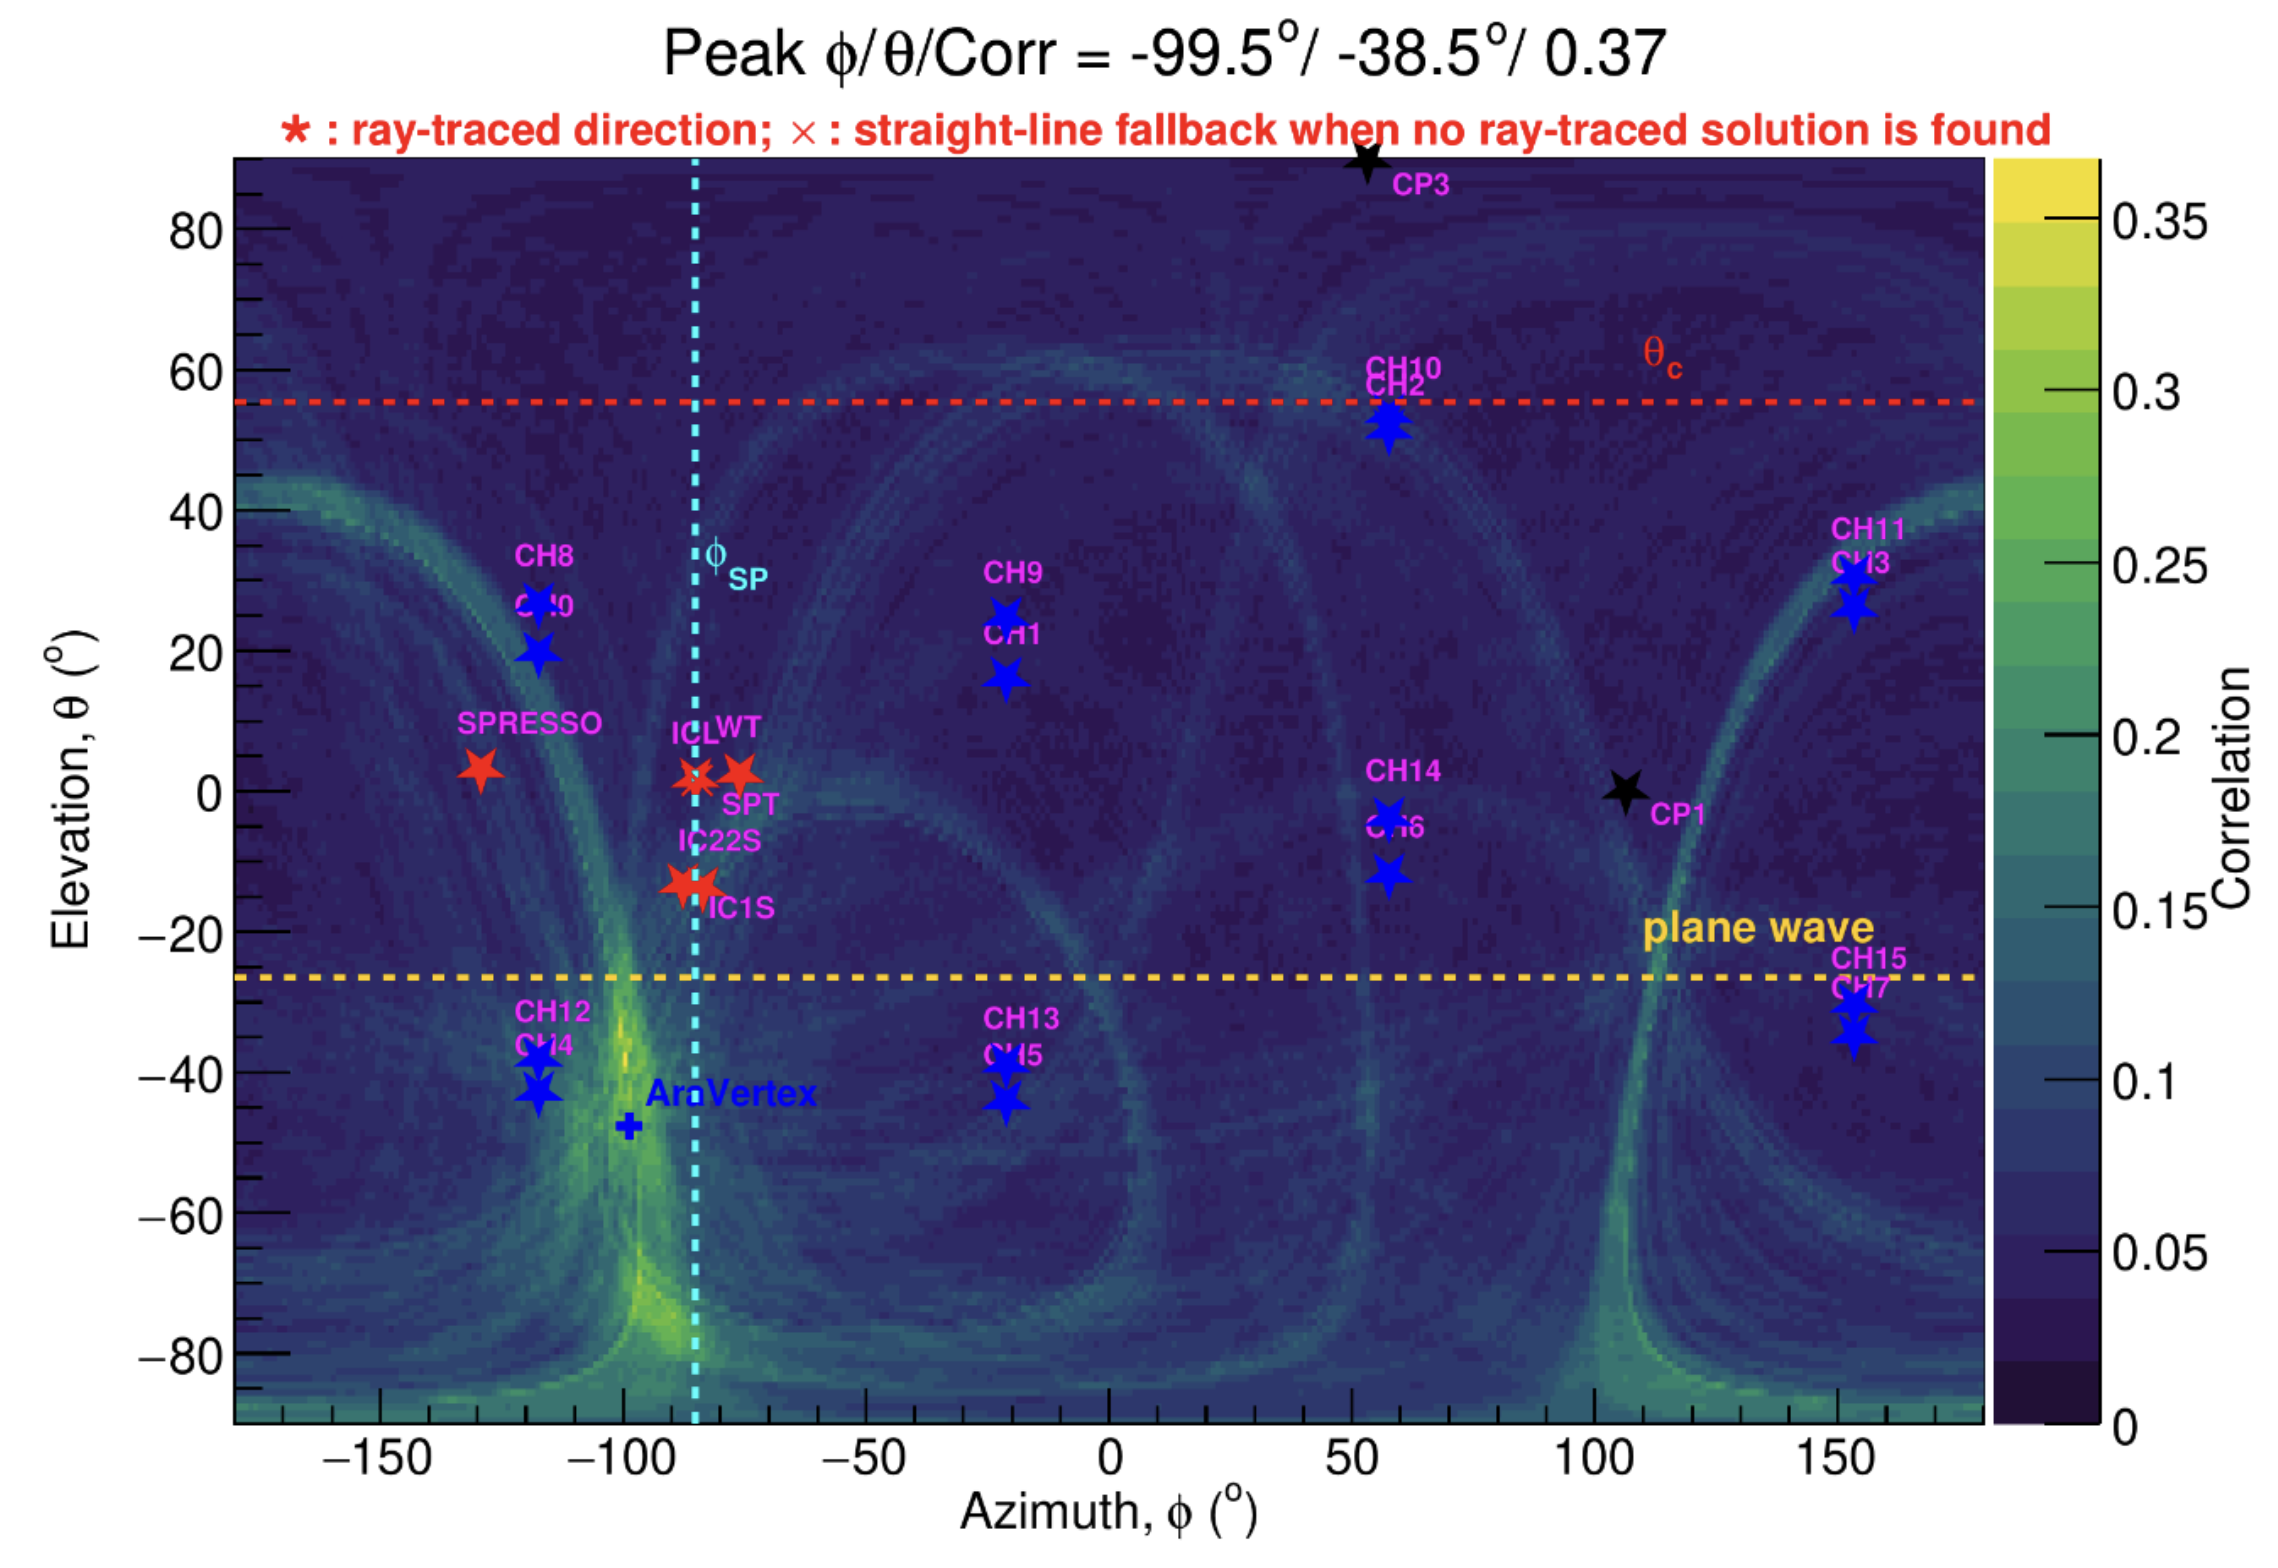
\includegraphics[
          width=\linewidth,
          alt={}
        ]{sections/5sa-analysis/images/passingevent_a5reco.png}
        \caption{
          Reconstruction of the A5 run 2899 event 64066, the event that occurred at the same time as the PA passing event. 
          The cross-correlation score assuming the signals originated from $-175.5^{\circ}\leq \phi \leq 175.5^{\circ}$ (x-axis) and $-89.5^{\circ}\leq \theta \leq 89.5^{\circ}$ (y-axis) are shown as a heat map.
          The location with the greatest correlation score is located at ($-99.5^{\circ}$, $-38.5^{\circ}$).
          The hit-time based reconstruction algorithm, \texttt{AraVertex}, reconstructs the event around ($-100^{\circ}$, $-48^{\circ}$) and is marked with a blue cross.
          Reconstruction assuming a plane wave solution estimates the signal originated from an elevation of $-26^{\circ}$ as is shown with the yellow, dashed line.
          All reconstructions suggest the event originates within $20^{\circ}$ in elevation (and azimuth for the interferometric and hit-time based reconstructions) of the A5 antennas 4 and 12 located around ($-120^{\circ}$, $-40^{\circ}$), marked with blue stars. 
        }
        \label{fig:passing_a5reco}
      \end{figure}

      Since the signals in the PA string and A5 strings 2, 3, and 4 resembled calibration pulsers but didn't reconstruct where we expect calibration pulses to come from, we added the locations of A5 and PA antennas to the reconstruction skymaps as shown in Fig~\ref{fig:passing_a5reco}.
      This showed that the AraVertex algorithm reconstructed the A5 event within $20^{\circ}$ of the locations of antennas 4 and 12. 
      The same effect was observed when we plotted the skymap of correlation scores for the A5 event's interferometric reconstruction using a map radius equal to the distance between A5 antenna 4 and the station center - the best interferometric reconstruction is $20^{\circ}$ away from the locations of antenna 4 and 12. 
      We repeated this exercise for the A4 event shown in Fig.~\ref{fig:a4outlier} and found the event reconstructed where antennas 6 and 14 are, the same channels exhibiting power surge behavior.
      The analysis presented in Ref.~\citep{ara_a23} also discovered 7 events of this nature which gave rise to the original Spark Event Cut.% \footnote{\url{https://aradocs.wipac.wisc.edu/cgi-bin/DocDB/ShowDocument?docid=2032}}.

      The impulsive signatures on the strings presented in Fig.~\ref{fig:a4outlier} were not understood when designing the Anomalous Channel Cut, but would not be classified as potential neutrino observations given the string of anomalous waveforms in the same event. 
      The anomalous waveforms were assumed to have been created by the data acquisition board which is housed in the vault at the surface, but as the impulsive signals in the same event resemble coherent radio emission reconstructing in deep ice, this suggests that the technical malfunction occurs on the string itself near the antennas. 
      This may be caused by the low noise amplifiers which are connected to and located next to each antenna, which can push power into the connected antenna, causing the antennas to temporally and spontaneously pulse radio waves like the calibration pulsers do.
      This may also be related to horizontally polarized antenna feeds, since no events like these occur after the 2019-2020 South Pole summer season.
      This was the season when all vertically polarized A5 antennas were connected to the PA data acquisition board and most horizontally polarized A5 antennas were left disconnected after the A5 board malfunctioned and stopped taking data (see Section~\ref{sec:pa_hardware} for more information).

      Based on these findings, an a posteriori cut was defined and applied to remove this class of technical backgrounds.
      We employ a cut that removes PA events within 0.05 seconds of A5 events that are cut by the Spark Event Cut defined in Section~\ref{sec:sec} or the Anomalous Channel Cut defined in Section~\ref{sec:acc}.
      219 A5 events were removed from the full sample by these cuts, leading to a negligible decrease in PA livetime of 21.9 seconds. 
      With the A1-A5 Anomalous Channel cut expanded to exclude nearby PA events, this event, which is clearly technical background, no longer passes all cuts and is rejected by this analysis.

      We have not found an explanation for why the A4 event occurred at the same time as the PA event which passed the analysis (and the corresponding A5 event).
      Over the whole array and livetime, the number of events removed by the Spark Event and Anomalous Channel cut is 13 for A1, 150 for A2, 90 for A3, 202 for A4, and 219 for A5. 
      Of these events, there were at most 3 coincident events across stations so we expect the simultaneous A4 and A5+PA spark events was a rare occurrence, though we have not completely ruled out that the A4 and A5 events were not random.
      User login records for the South Pole remote access computer for April 4, 2018 indicate there was an active user at the time of the PA passing event, but they were not affiliated with ARA, so it is unlikely that the events were associated with this person.
  
\section{Results\label{sec:5sa_results}}

    In absence of an observed neutrino event, we construct an upper limit on the observed neutrino flux.
    The 90\% confidence level upper limit factor relies on the number of observed events (0, for this analysis) and the number of expected backgrounds. 
    We modeled backgrounds for the Geometry Cut, the Zenith Cut, and the LDA Cut.
    As discussed in Section~\ref{sec:gc}, the windows used in the Geometry Cut were defined such that the number of passing events was $2\times10^{-5}$ for the 10\% sample, meaning $2\times10^{-4}$ for the 100\% sample. 
    We multiply this by our expected untagged calibration pulser event rate of $10^{-4}$ for each station to achieve a background leakage of $2\times 10^{-8}$ events per window.  
    For both the Zenith Cut and LDA Cut, the number of expected background events is an output from the optimization performed in Section~\ref{sec:optimization}. 
    The number of background events per station and array-wide are presented in Table~\ref{tab:backgrounds}.

    \begin{figure}
      \centering
      \includegraphics[
        width=\linewidth,
        alt={}
      ]{sections/5sa-analysis/images/Background-Leakage.pdf}
      \caption{
        The number of background events expected (based on the fits to 10\% of the data) to ``leak'' into the final dataset based on the Geometry Cut and models defined in Section~\ref{sec:gc}, the Zenith Cut defined in Section~\ref{sec:zc_slc} and Optimized in Section~\ref{sec:optimization}, and the thermal-like LDA cut defined in Section~\ref{sec:lda} and optimized in Section~\ref{sec:optimization}.
        The number of leaked events is presented per station and for the array as a whole.
      }
      \label{tab:backgrounds}
    \end{figure}

    The final upper limit of this analysis is established using the simulations defined in Chapter~\ref{chap:veff} and Eq.~\ref{eq:phi_UL} and is reported in Tab~\ref{tab:results}.

    \begin{table}[ht!]
      \centering
      \begin{tabular}{|c|c|}
        \hline
        & $N_{\text{events}}$ \\
        \hline
        Background & 0.13 \\
        Observed & 0 \\
        90\% CL Upper Limit & 2.44 \\
        \hline
      \end{tabular}
      \caption{
        Expected number of background events, observed number of events that passed this analysis, and the \citep{feldman_cousins} 90\% confidence level upper limit on the number of events for this analysis.
      }
      \label{tab:results}
    \end{table}

    The differential upper limit to the cosmic neutrino flux is shown as the bold line in Fig.~\ref{fig:5sa_sensitivity}, with the analysis' Single Event Sensitivity (SES) and trigger level upper limit. 
    % We establish 90\% confidence when stating that the true rate of neutrinos in each energy bin could be up to 2.44, according to the Feldman Cousins formulation.
    The SES represents the flux required to observe at least 1 event in each energy bin.
    The number of events we predict exist in our sample after all cuts have been applied is given in Tab.~\ref{tab:5sa_eventrates}.
    The sensitivity achieved by this analysis can be compared to results by other experiments and a collection of neutrino flux models, including the models that yield the greatest neutrino flux from \citep{flux-kotera,flux-muzio,flux-ahlers-halzen}.

    \begin{figure}
        \centering
        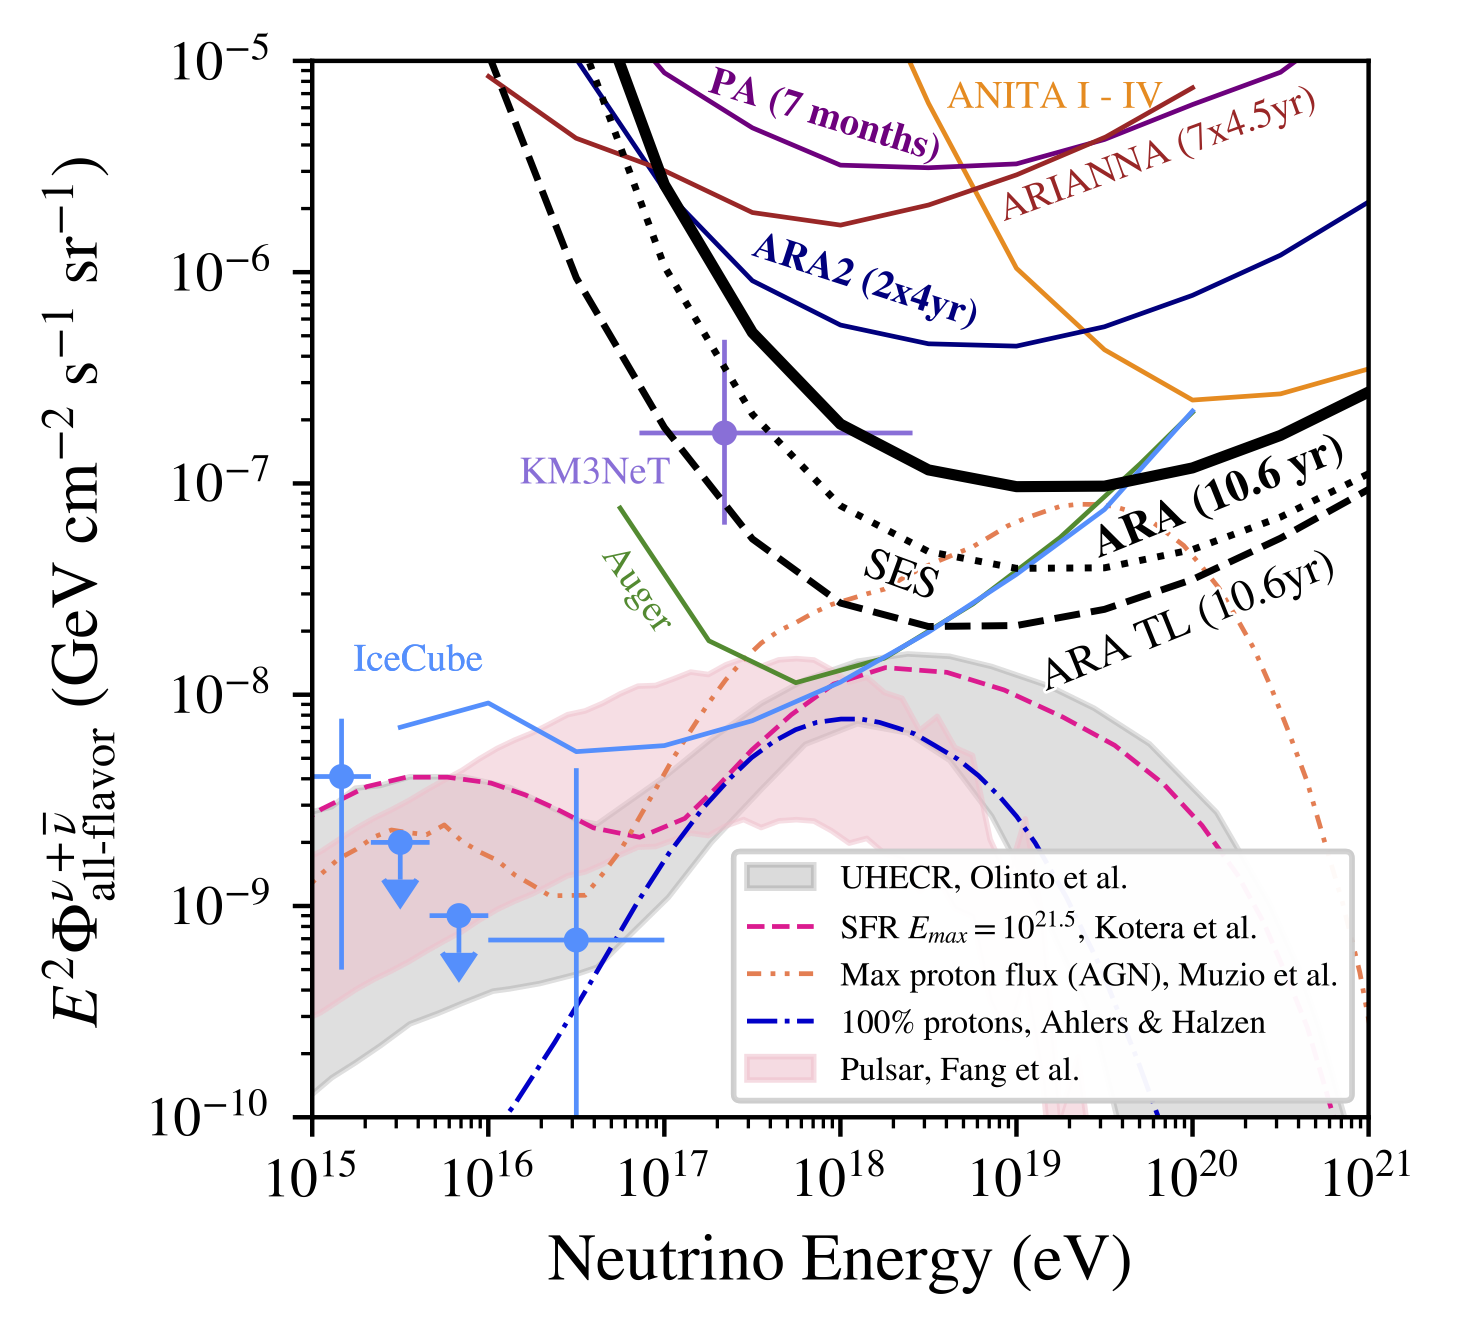
\includegraphics[
            width=0.75\textwidth,
            alt={}
        ]{sections/5sa-analysis/images/5sa_e2Sensitivity_astrocosmo-5SA.pdf}
        \caption{
          Analysis level sensitivity of the array-wide neutrino search through 10.6 years of ARA data (solid black curve). 
          The single event sensitivity (SES) of the analysis level sensitivity is also presented (dotted black curve) along with the trigger level sensitivity (ARA TL, dashed black curve).
          Previous experimental results from IceCube~\citep{icecube_search-ehe, icecube_search-combined-fit}, KM3NeT~\citep{km3net_neutrino}, Auger~\citep{flux-auger}, ARIANNA~\citep{arianna_testbed}, ANITA I--IV~\citep{anita_iv}, and earlier ARA analyses (ARA2~\citep{ara_a23} and PA~\citep{ara_pa_analysis}) are also shown (colored solid).
          A selection of optimistic cosmogenic and astrophysical neutrino flux models are presented as well~\citep{flux-kotera,flux-muzio,flux-ahlers-halzen,flux-fang-pulsars, flux_olinto}.
        }
        \label{fig:5sa_sensitivity}
    \end{figure}

    \begin{table}
      \centering
      \begin{tabular}{ 
          >{\centering\arraybackslash}m{5cm} 
          >{\centering\arraybackslash}m{3cm} | 
          >{\centering\arraybackslash}m{3cm} 
          >{\centering\arraybackslash}m{3cm} 
        }
        Model & Model Type & $N_{\text{events}}$ \hspace{0.5cm} (Trigger Level) & $N_{\text{events}}$ \hspace{0.5cm}  (Analysis Level) \\
        \hline
        \hline
        Global Upper Limit \citep{icecube_search-ehe, anita_iv} & Experimental & 21.64 & 6.24 \\
        \citep{flux-muzio} & Cosmogenic & 12.11 & 2.79 \\
        \citep{flux-kotera} & Cosmogenic & 2.09 & 0.41 \\
        100\% Protons \citep{flux-ahlers-halzen} & Cosmogenic & 0.87 & 0.15 \\
        \citep{flux-fang-pulsars} & Astrophysical & 1.31 & 0.20 \\
        \citep{km3net_neutrino} & Experiment & 12.30 & 1.73 \\
        \citep{icecube_search_extension} & Experiment & 0.19 & 0.03 \\
      \end{tabular}
      \caption{
        Expected number of neutrino events expected at trigger level and at analysis level based on various astrophysical models, cosmogenic models, and experimental fluxes and upper limits. 
        These results may be compared to the Feldman-Cousins upper limit of 2.44 events, established by the observation of 0 events on an expected background of 0.13 events in this analysis.
      }
      \label{tab:5sa_eventrates}
    \end{table}

%% etc, etc.

%% Do you have appendices?  If so, add them here, just like chapters.
\begin{appendices}
    \chapter{5 Station Analysis L2 Variables \label{app:5savariables}}

This is a limited collection of analysis variables calculated as a part of the analysis presented in Chapter~\ref{chap:5sa_cleaning} and Chapter~\ref{chap:5sa_analysis}. 
Full definitions of each variable may be found in AraProc source code.

\section{\texttt{avg\_rms} \label{sec:rms}}

  The average root-mean-square ($RMS$, also referred to as $\sigma$) of noise portions of waveforms is calculated using a jackknife technique. 
  The full waveform is split into 50 segments and the RMS of the waveform without each segment is calculated in the so-called $RMS_{\text{all-but}}$. 
  Segments that contain non-thermal signals have an $RMS_{\text{all-but}}$ that is significantly less than the average of $RMS_{\text{all-but}}$ values for all segments. 
  Segments with an $RMS_{\text{all-but}}$ value more than one standard deviation lower than the mean of all other $RMS_{\text{all-but}}$ values are isolated. 
  Once all segments with non-thermal contributions are isolated, the $RMS$ is calculated over all remaining segments. 

  \begin{figure}
    \centering
    \begin{subfigure}[t]{0.48\textwidth}
      \centering
      \includegraphics[width=\textwidth]{sections/5sa-cleaning/images_variables/a2nu_1d_avg_rms_v.pdf}
    \end{subfigure}
    ~
    \begin{subfigure}[t]{0.48\textwidth}
      \centering
      \includegraphics[width=\textwidth]{sections/5sa-cleaning/images_variables/a2_10pct_1d_avg_rms_v.pdf}
    \end{subfigure}
    ~
    \begin{subfigure}[t]{0.48\textwidth}
      \centering
      \includegraphics[width=\textwidth]{sections/5sa-cleaning/images_variables/a2nu_2d_avg_rms_v_vs_avg_snr_v_rf.pdf}
    \end{subfigure}
    ~
    \begin{subfigure}[t]{0.48\textwidth}
      \centering
      \includegraphics[width=\textwidth]{sections/5sa-cleaning/images_variables/a2nu_2d_avg_rms_v_vs_global_max_corr_rf.pdf}
    \end{subfigure}
    \caption{
      Top, 1-dimensional distributions of simulated neutrinos following an $E^{-2}$ spectrum (top left) and data (top right) for the analysis variable \texttt{avg\_rms\_v}. 
      The distribution of data has had all cuts applied to RF events except for the final thermal LDA cut described in Section~\ref{sec:lda}.
      The purple curve (which exactly overlays the orange curve) shows these RF events, blue shows software triggered events, and green shows calibration pulser events.
      Bottom, 2-dimensional distributions of simulated neutrinos for the analysis variable \texttt{avg\_rms\_v} as a function of \texttt{avg\_snr\_v} and \texttt{global\_max\_corr\_v}.
    }
    \label{fig:avg_rms}
  \end{figure}

\pagebreak
\section{\texttt{avg\_rpr} and \texttt{csw\_rpr}}

    The root power ratio ($RPR$) approximates the maximum power in a waveform and divides it by the voltage of the noise background, in a calculation similar to the signal-to-noise ratio ($SNR$).
    The $RPR$ is calculated two ways, first by squaring the raw waveform, squaring each value (as the proxy for power), smoothing the squared waveform, and extracting the maximum value then dividing it by the $RMS$ of the noise background in the waveform via the calculation defined in Section~\ref{sec:rms}.
    The second method follows the same approach but uses the Coherently Summed Waveform instead of the raw waveform to perform the calculation.
    For both methods, the average $RPR$ is calculated over all like-polarization channels and returned.
    Example distributions are shown in Figure~\ref{fig:avg_rpr}.
  
    \begin{figure}
      \centering
      \begin{subfigure}[t]{0.48\textwidth}
        \centering
        \includegraphics[width=\textwidth]{sections/5sa-cleaning/images_variables/a2nu_1d_avg_rpr_v.pdf}
      \end{subfigure}
      ~
      \begin{subfigure}[t]{0.48\textwidth}
        \centering
        \includegraphics[width=\textwidth]{sections/5sa-cleaning/images_variables/a2_10pct_1d_avg_rpr_v.pdf}
      \end{subfigure}
      ~
      \begin{subfigure}[t]{0.48\textwidth}
        \centering
        \includegraphics[width=\textwidth]{sections/5sa-cleaning/images_variables/a2nu_2d_avg_rpr_v_vs_avg_snr_v_rf.pdf}
      \end{subfigure}
      ~
      \begin{subfigure}[t]{0.48\textwidth}
        \centering
        \includegraphics[width=\textwidth]{sections/5sa-cleaning/images_variables/a2nu_2d_avg_rpr_v_vs_global_max_corr_rf.pdf}
      \end{subfigure}
      \caption{
        Top, 1-dimensional distributions of simulated neutrinos following an $E^{-2}$ spectrum (top left) and data (top right) for the analysis variable \texttt{avg\_rpr\_v}. 
        The distribution of data has had all cuts applied to RF events except for the final thermal LDA cut described in Section~\ref{sec:lda}.
        The purple curve (which exactly overlays the orange curve) shows these RF events, blue shows software triggered events, and green shows calibration pulser events.
        Bottom, 2-dimensional distributions of simulated neutrinos for the analysis variable \texttt{avg\_rpr\_v} as a function of \texttt{avg\_snr\_v} and \texttt{global\_max\_corr\_v}.
      }
      \label{fig:avg_rpr}
    \end{figure}

\pagebreak
\section{\texttt{avg\_s2}}

  \texttt{avg\_s2} is a measure of signal causality constructed similarly to the \texttt{wavefront\_rms}. 
  For all antennas of like-polarization, the time of maximum peak-to-peak voltage in any 20 nanosecond window of every waveform is identified. 
  Again assuming that a plane wave arrived at each antenna at the determined time of maximal voltage separation, for each pair of antennas we calculate the average spacetime interval as
  \begin{equation}
    s^2 = \Delta r^2 - ({c}{n})^2 \Delta t^2
    \label{eq:avg_s2}
  \end{equation}
  where $\Delta r$ is the distance between a pair of antennas, $c$ is the speed of light in a vacuum, $n$ is the index of refraction of the medium, and  $\Delta t$ is the time difference between the assumed signal arrival in each antenna (the time of maximal voltage separation).
  When $s^2$ is positive this indicates a causal relationship between signals in each channel. 
  When $s^2$ is negative, this indicates an acausal, non-physical signal that would not be expected of an arriving impulsive signal.
  We take the average $s^2$ calculated over all antenna pairs of like-polarization and report this as the \texttt{avg\_s2}.
  Example distributions are shown in Figure~\ref{fig:avg_s2}.

  \begin{figure}
    \centering
    \begin{subfigure}[t]{0.48\textwidth}
      \centering
      \includegraphics[width=\textwidth]{sections/5sa-cleaning/images_variables/a2nu_1d_avg_s2_v.pdf}
    \end{subfigure}
    ~
    \begin{subfigure}[t]{0.48\textwidth}
      \centering
      \includegraphics[width=\textwidth]{sections/5sa-cleaning/images_variables/a2_10pct_1d_avg_s2_v.pdf}
    \end{subfigure}
    ~
    \begin{subfigure}[t]{0.48\textwidth}
      \centering
      \includegraphics[width=\textwidth]{sections/5sa-cleaning/images_variables/a2nu_2d_avg_s2_v_vs_avg_snr_v_rf.pdf}
    \end{subfigure}
    ~
    \begin{subfigure}[t]{0.48\textwidth}
      \centering
      \includegraphics[width=\textwidth]{sections/5sa-cleaning/images_variables/a2nu_2d_avg_s2_v_vs_global_max_corr_rf.pdf}
    \end{subfigure}
    \caption{
      Top, 1-dimensional distributions of simulated neutrinos following an $E^{-2}$ spectrum (top left) and data (top right) for the analysis variable \texttt{avg\_s2\_v}. 
      The distribution of data has had all cuts applied to RF events except for the final thermal LDA cut described in Section~\ref{sec:lda}.
      The purple curve (which exactly overlays the orange curve) shows these RF events, blue shows software triggered events, and green shows calibration pulser events.
      Bottom, 2-dimensional distributions of simulated neutrinos for the analysis variable \texttt{avg\_s2\_v} as a function of \texttt{avg\_snr\_v} and \texttt{global\_max\_corr\_v}.
    }
    \label{fig:avg_s2}
  \end{figure}

\pagebreak
\section{\texttt{avg\_snr}}
  
    The average signal-to-noise ratio ($SNR$) is calculated using Equation~\ref{eq:snr} by identifying the maximum peak-to-peak voltage ($V_{\text{max}} - V_{\text{min}}$) within an 20~ns window, dividing this value by two (to quantify the amount of ``signal'' in the waveform), then dividing this number by the $RMS$ voltage for the waveform as defined in Section~\ref{sec:rms} (to quantify the ``noise'', also referred to as $\sigma$).
    The $SNR$ values in each like-polarization channel are averaged together to achieve the average $SNR$.
    Example distributions are shown in Figure~\ref{fig:avg_snr}.
  
    \begin{figure}
      \centering
      \begin{subfigure}[t]{0.48\textwidth}
        \centering
        \includegraphics[width=\textwidth]{sections/5sa-cleaning/images_variables/a2nu_1d_avg_snr_v.pdf}
      \end{subfigure}
      ~
      \begin{subfigure}[t]{0.48\textwidth}
        \centering
        \includegraphics[width=\textwidth]{sections/5sa-cleaning/images_variables/a2_10pct_1d_avg_snr_v.pdf}
      \end{subfigure}
      ~
      \begin{subfigure}[t]{0.48\textwidth}
        \centering
        \includegraphics[width=\textwidth]{sections/5sa-cleaning/images_variables/a2nu_2d_global_max_corr_vs_avg_snr_v_rf.pdf}
      \end{subfigure}
      \caption{
        Top, 1-dimensional distributions of simulated neutrinos following an $E^{-2}$ spectrum (top left) and data (top right) for the analysis variable \texttt{avg\_snr\_v}. 
        The distribution of data has had all cuts applied to RF events except for the final thermal LDA cut described in Section~\ref{sec:lda}.
        The purple curve (which exactly overlays the orange curve) shows these RF events, blue shows software triggered events, and green shows calibration pulser events.
        Bottom, 2-dimensional distributions of simulated neutrinos for the analysis variable \texttt{avg\_snr\_v} as a function of \texttt{global\_max\_corr\_v}.
      }
      \label{fig:avg_snr}
    \end{figure}
  
\section{\texttt{corr\_snr}}

  The correlation $SNR$ is calculated by identifying all pairs of like-polarization channels, calculating the cross correlation function of their two waveforms, then determining the SNR (following Equation~\ref{eq:snr}) of the cross correlation function for each pair. 
  The average over the SNR for each pair's correlation function is what is returned as the \texttt{corr\_snr}.
  Example distributions are shown in Figure~\ref{fig:corr_snr}.
  
  \begin{figure}
    \centering
    \begin{subfigure}[t]{0.48\textwidth}
      \centering
      \includegraphics[width=\textwidth]{sections/5sa-cleaning/images_variables/a2nu_1d_corr_snr_v.pdf}
    \end{subfigure}
    ~
    \begin{subfigure}[t]{0.48\textwidth}
      \centering
      \includegraphics[width=\textwidth]{sections/5sa-cleaning/images_variables/a2_10pct_1d_corr_snr_v.pdf}
    \end{subfigure}
    ~
    \begin{subfigure}[t]{0.48\textwidth}
      \centering
      \includegraphics[width=\textwidth]{sections/5sa-cleaning/images_variables/a2nu_2d_corr_snr_v_vs_avg_snr_v_rf.pdf}
    \end{subfigure}
    ~
    \begin{subfigure}[t]{0.48\textwidth}
      \centering
      \includegraphics[width=\textwidth]{sections/5sa-cleaning/images_variables/a2nu_2d_corr_snr_v_vs_global_max_corr_rf.pdf}
    \end{subfigure}
    \caption{
      Top, 1-dimensional distributions of simulated neutrinos following an $E^{-2}$ spectrum (top left) and data (top right) for the analysis variable \texttt{corr\_snr\_v}. 
      The distribution of data has had all cuts applied to RF events except for the final thermal LDA cut described in Section~\ref{sec:lda}.
      The purple curve (which exactly overlays the orange curve) shows these RF events, blue shows software triggered events, and green shows calibration pulser events.
      Bottom, 2-dimensional distributions of simulated neutrinos for the analysis variable \texttt{corr\_snr\_v} as a function of \texttt{avg\_snr\_v} and \texttt{global\_max\_corr\_v}.
    }
    \label{fig:corr_snr}
  \end{figure}
  
\pagebreak
\section{\texttt{csw\_snr} \label{sec:csw}}
  
    \begin{figure}[!ht]
      \centering
      \centering
      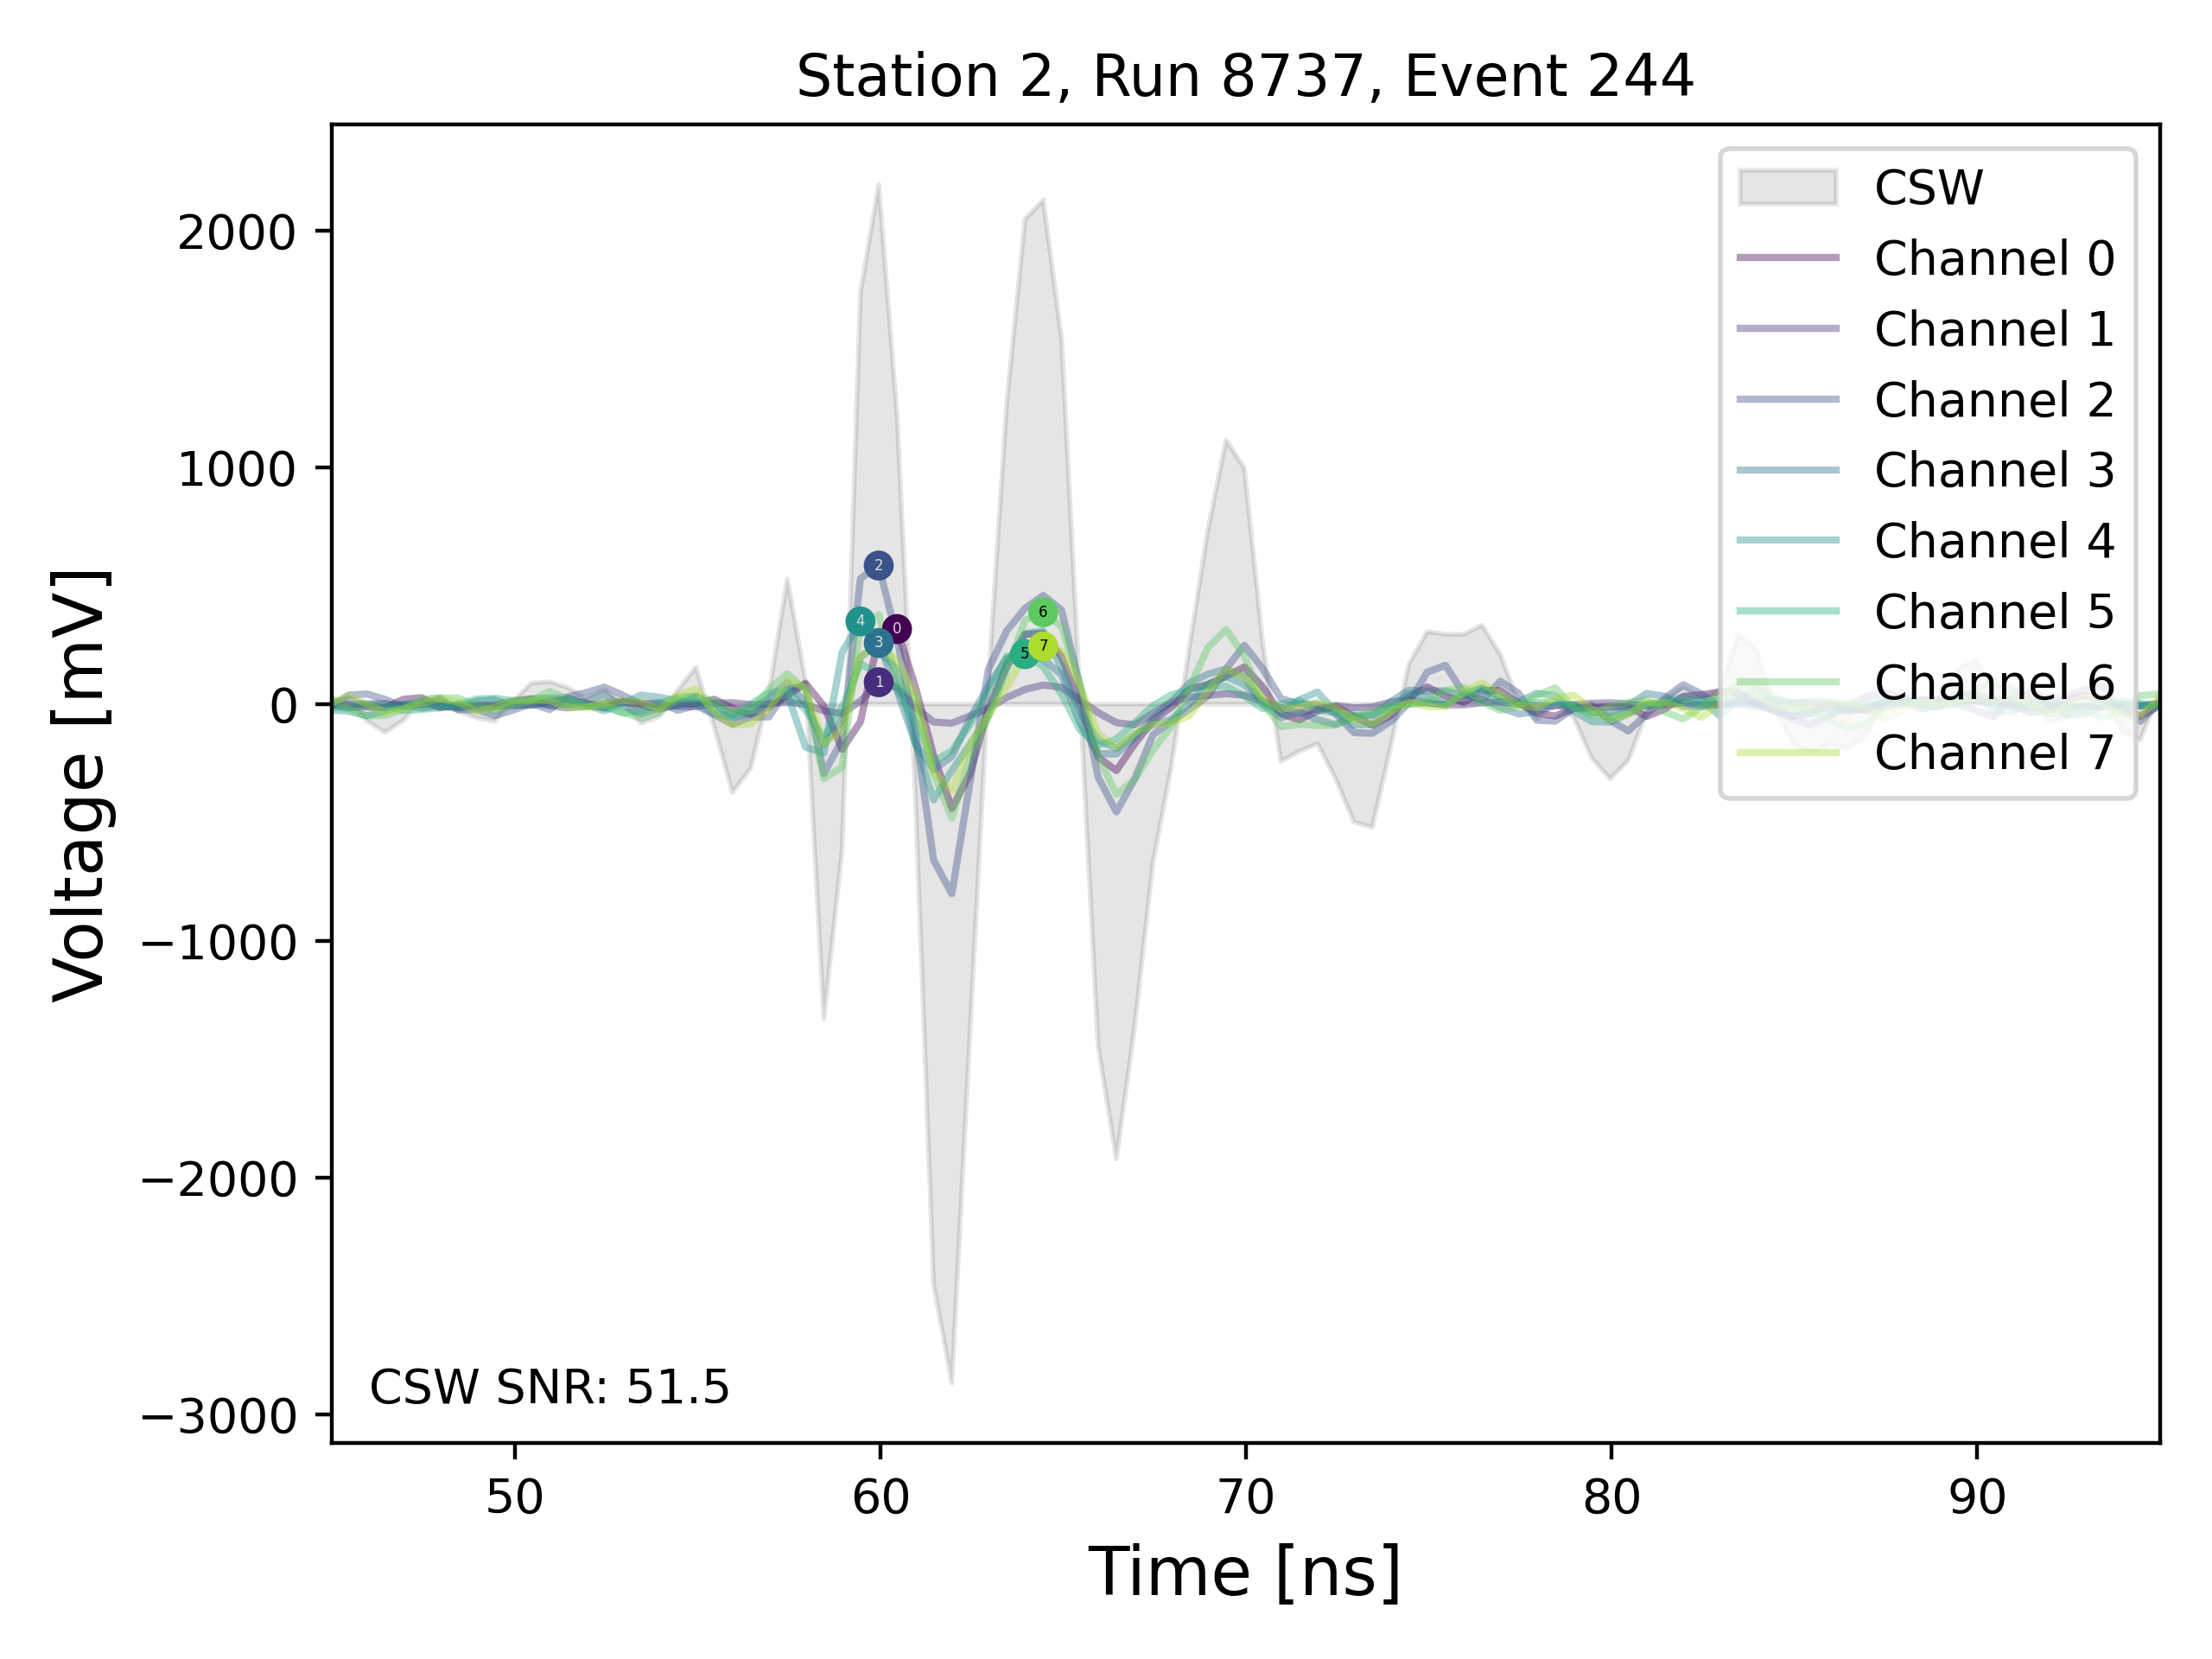
\includegraphics[width=0.75\textwidth]{sections/5sa-cleaning/images_variables/csw_s2_r8737_e244.png}
      \caption{
        Example of a Coherently Summed Waveform (CSW, grey) and the waveforms composing the CSW. 
        The circles on each channel mark the location of each waveform's maximum voltage.
      }
      \label{fig:csw}
    \end{figure}

    The Coherently Summed Waveform (CSW) SNR is calculated by determining the SNR of the CSW composed of all like-polarization antennas. 
    The CSW is constructed first by reconstructing an events arrival direction using the interferometric reconstruction algorithm described in Section~\ref{sec:reco}. 
    The expected arrival time of signals from this reconstructed location to each like-polarization antenna are used to translate each waveform in time. 
    For highly correlated signals, the peak of each waveform should now align at the same time bin. 
    When each waveform is added together, the signal increases roughly at a factor of $N_a$ (the number of antennas) but the noise increases at a factor of roughly $\sqrt{N_a}$. 
    This allows highly correlated signals that are low in signal strength to rise out of the noise floor, increasing their chance of passing all analysis cuts. 
    Before summing all waveforms, each waveform's time delay is allowed to change by up to 20~ns to maximize the CSW.
    An example of a CSW is shown in Figure~\ref{fig:csw} and example distributions are shown in Figure~\ref{fig:csw_snr}.
  
    \begin{figure}
      \centering
      \begin{subfigure}[t]{0.48\textwidth}
        \centering
        \includegraphics[width=\textwidth]{sections/5sa-cleaning/images_variables/a2nu_1d_csw_snr_v.pdf}
      \end{subfigure}
      ~
      \begin{subfigure}[t]{0.48\textwidth}
        \centering
        \includegraphics[width=\textwidth]{sections/5sa-cleaning/images_variables/a2_10pct_1d_csw_snr_v.pdf}
      \end{subfigure}
      ~
      \begin{subfigure}[t]{0.48\textwidth}
        \centering
        \includegraphics[width=\textwidth]{sections/5sa-cleaning/images_variables/a2nu_2d_csw_snr_v_vs_avg_snr_v_rf.pdf}
      \end{subfigure}
      ~
      \begin{subfigure}[t]{0.48\textwidth}
        \centering
        \includegraphics[width=\textwidth]{sections/5sa-cleaning/images_variables/a2nu_2d_csw_snr_v_vs_global_max_corr_rf.pdf}
      \end{subfigure}
      \caption{
        Top, 1-dimensional distributions of simulated neutrinos following an $E^{-2}$ spectrum (top left) and data (top right) for the analysis variable \texttt{csw\_snr\_v}. 
        The distribution of data has had all cuts applied to RF events except for the final thermal LDA cut described in Section~\ref{sec:lda}.
        The purple curve (which exactly overlays the orange curve) shows these RF events, blue shows software triggered events, and green shows calibration pulser events.
        Bottom, 2-dimensional distributions of simulated neutrinos for the analysis variable \texttt{csw\_snr\_v} as a function of \texttt{avg\_snr\_v} and \texttt{global\_max\_corr\_v}.
      }
      \label{fig:csw_snr}
    \end{figure}

\pagebreak
\section{\texttt{global\_max\_corr} and \texttt{reco\_result\_*\_corr}}
  
  The cross correlation of all pairs of like-polarized antennas is performed on a sphere with a radius equal to the pulser's distance from the station's center (this is also called the ``nearby" reconstruction) and a sphere with a radius of 300 meters (called the ``distant" reconstruction). 
  %The reconstructed correlation is computed by determining which point on the sphere the signals must have come from to be maximally correlated.
  %The correlation is first computed between pairs of antennas where waveforms have been shifted in time according to the arrival delay of signals if they were to arrive from a certain location on the sphere. 
  %Once time-shifted, the two waveforms are cross correlated to obtain their correlation value. 
  %% What is the correlation? The maximum of the correlation function or the area under the curve or what? 
  %% Is the total correlation an average of the correlation between all antennas? 
  %It is a process that requires significant computation time as multiple locations on the sphere are tested in search of the best position on the sphere. 
  
  The maximum correlation in all four reconstructions (two polarizations, two distances) is saved to a variable called \texttt{global\_max\_corr} while the maximum correlation in horizontally and vertically polarized antennas separately are saved as \texttt{global\_max\_corr\_h} and \texttt{global\_max\_corr\_v}, respectively. Shown in Figure~\ref{fig:global_max_correlation} are example distributions of the \texttt{global\_max\_corr} variable.
  
    \begin{figure}
      \centering
      \begin{subfigure}[t]{0.48\textwidth}
        \centering
        \includegraphics[width=\textwidth]{sections/5sa-cleaning/images_variables/a2nu_1d_global_max_corr.pdf}
      \end{subfigure}
      ~
      \begin{subfigure}[t]{0.48\textwidth}
        \centering
        \includegraphics[width=\textwidth]{sections/5sa-cleaning/images_variables/a2_10pct_1d_global_max_corr.pdf}
      \end{subfigure}
      ~
      \begin{subfigure}[t]{0.48\textwidth}
        \centering
        \includegraphics[width=\textwidth]{sections/5sa-cleaning/images_variables/a2nu_2d_global_max_corr_vs_avg_snr_v_rf.pdf}
      \end{subfigure}
      \caption{
        Top, 1-dimensional distributions of simulated neutrinos following an $E^{-2}$ spectrum (top left) and data (top right) for the analysis variable \texttt{global\_max\_corr}. 
        The distribution of data has had all cuts applied to RF events except for the final thermal LDA cut described in Section~\ref{sec:lda}.
        The purple curve (which exactly overlays the orange curve) shows these RF events, blue shows software triggered events, and green shows calibration pulser events.
        Bottom, 2-dimensional distributions of simulated neutrinos for the analysis variable \texttt{global\_max\_corr} as a function of \texttt{avg\_snr\_v}.
      }
      \label{fig:global_max_correlation}
    \end{figure}

\section{\texttt{hilbert\_snr}}

    The Hillbert SNR is the average SNR of each waveform from like-polarized antennas after being Hilbert Enveloped. 
    Example distributions are show in in Figure~\ref{fig:hilbert_snr}.
  
    \begin{figure}
      \centering
      \begin{subfigure}[t]{0.48\textwidth}
        \centering
        \includegraphics[width=\textwidth]{sections/5sa-cleaning/images_variables/a2nu_1d_hilbert_snr_v.pdf}
      \end{subfigure}
      ~
      \begin{subfigure}[t]{0.48\textwidth}
        \centering
        \includegraphics[width=\textwidth]{sections/5sa-cleaning/images_variables/a2_10pct_1d_hilbert_snr_v.pdf}
      \end{subfigure}
      ~
      \begin{subfigure}[t]{0.48\textwidth}
        \centering
        \includegraphics[width=\textwidth]{sections/5sa-cleaning/images_variables/a2nu_2d_hilbert_snr_v_vs_avg_snr_v_rf.pdf}
      \end{subfigure}
      ~
      \begin{subfigure}[t]{0.48\textwidth}
        \centering
        \includegraphics[width=\textwidth]{sections/5sa-cleaning/images_variables/a2nu_2d_hilbert_snr_v_vs_global_max_corr_rf.pdf}
      \end{subfigure}
      \caption{
        Top, 1-dimensional distributions of simulated neutrinos following an $E^{-2}$ spectrum (top left) and data (top right) for the analysis variable \texttt{hilbert\_snr\_v}. 
        The distribution of data has had all cuts applied to RF events except for the final thermal LDA cut described in Section~\ref{sec:lda}.
        The purple curve (which exactly overlays the orange curve) shows these RF events, blue shows software triggered events, and green shows calibration pulser events.
        Bottom, 2-dimensional distributions of simulated neutrinos for the analysis variable \texttt{hilbert\_snr\_v} as a function of \texttt{avg\_snr\_v} and \texttt{global\_max\_corr\_v}.
      }
      \label{fig:hilbert_snr}
    \end{figure}

\pagebreak
\section{\texttt{*imp*}}

    All impulsivity metrics are calculated using the cumulative distribution function (CDF) of the Hilbert enveloped CSW (defined in Section~\ref{sec:csw}) integrated outwards from the maximum point in the Hilbert enveloped waveform.
    Examples of these so-called impulsivity CDFs for an impulsive event, a perfectly impulsive (delta function) event, and a perfectly non-impulsive event are shown in Figure~\ref{fig:impulsivity_cdfs}.
  
    \begin{figure}[!ht]
      \centering
      \begin{subfigure}[t]{0.48\textwidth}
        \centering
        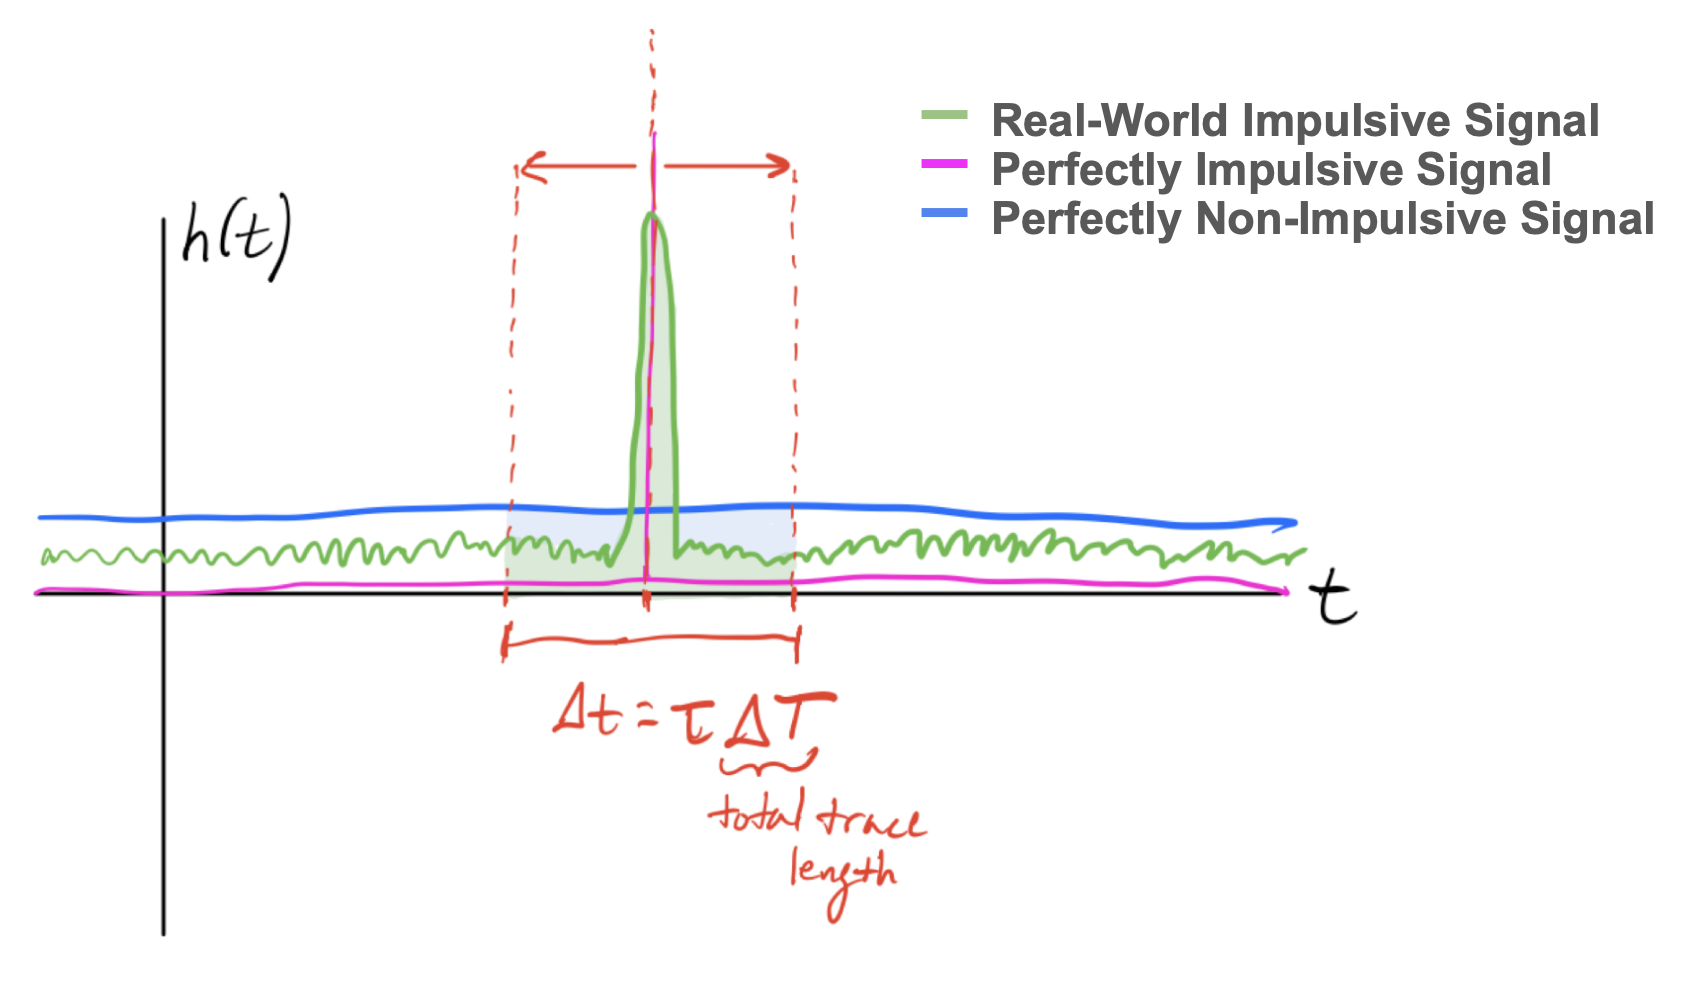
\includegraphics[width=\textwidth]{sections/5sa-cleaning/images_variables/impulsivity_waveforms.png}
      \end{subfigure}
      ~
      \begin{subfigure}[t]{0.48\textwidth}
        \centering
        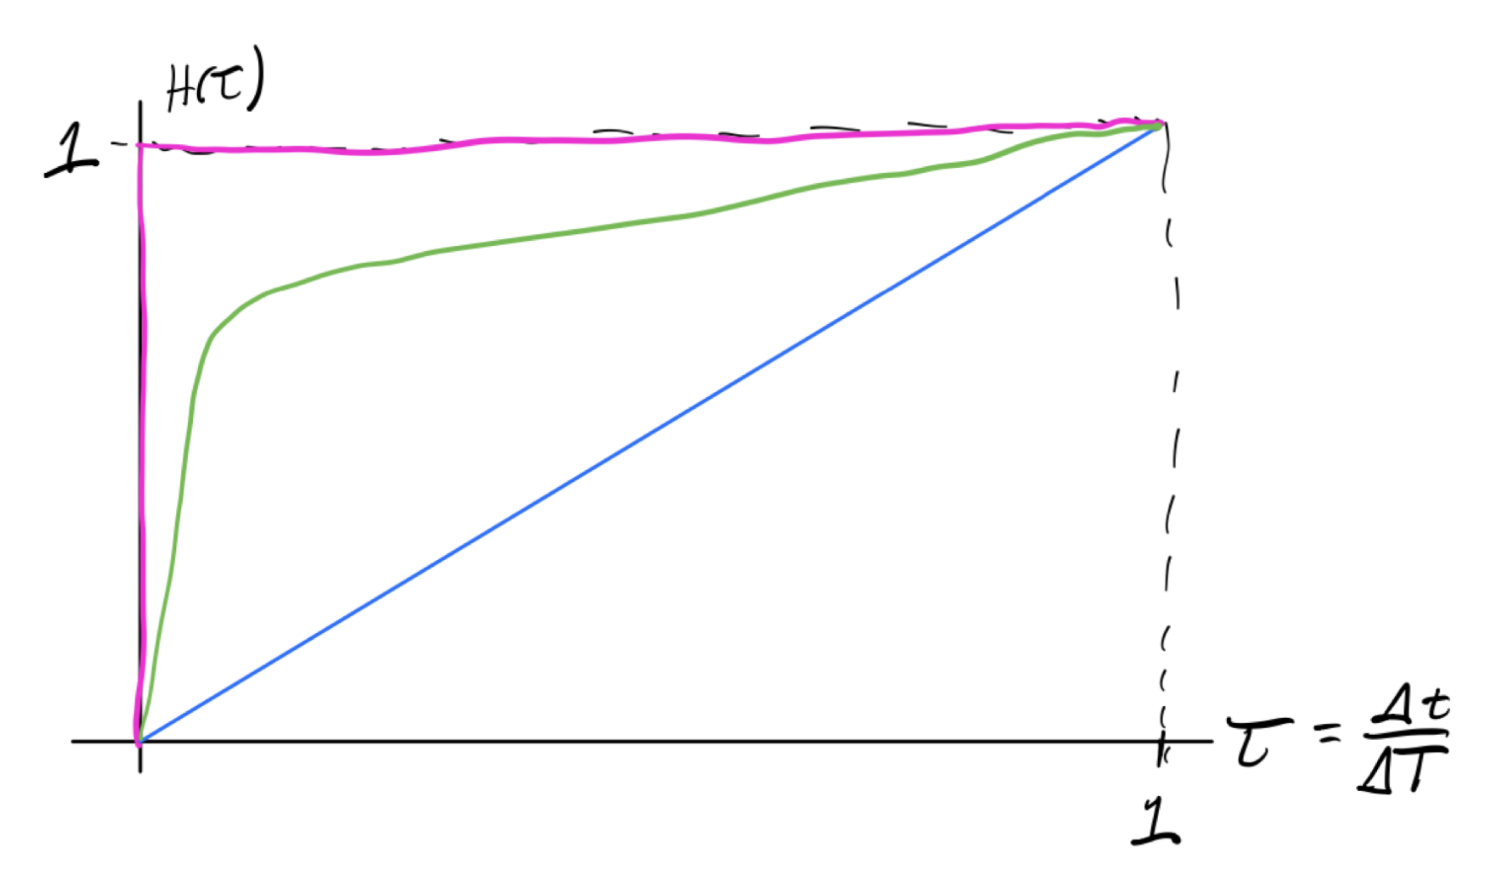
\includegraphics[width=\textwidth]{sections/5sa-cleaning/images_variables/impulsivity_cdfs.png}
      \end{subfigure}
      \caption{Left, cartoons of Hilbert enveloped waveforms for a real-world impulsive event (green), a perfectly impulsive event (pink), and a perfectly non-impulsive event. Right, cartoons of the corresponding impulsivity cumulative distribution function for each waveform shown on the left. }
      \label{fig:impulsivity_cdfs}
    \end{figure}

  \subsection{\texttt{impulsivity}}

      The impulsivity is calculated as 
      \begin{equation}
        \texttt{impulsivity} = \frac{1}{2} \overline{CDF} - 1
        \label{eq:impulsivity}
      \end{equation}
      where $\overline{CDF}$ is the average value of the impulsivity cumulative distribution function for this event's CSW.
      Example distributions are show in Figure~\ref{fig:impulsivity}.
    
      \begin{figure}
        \centering
        \begin{subfigure}[t]{0.48\textwidth}
          \centering
          \includegraphics[width=\textwidth]{sections/5sa-cleaning/images_variables/a2nu_1d_impulsivity_v.pdf}
        \end{subfigure}
        ~
        \begin{subfigure}[t]{0.48\textwidth}
          \centering
          \includegraphics[width=\textwidth]{sections/5sa-cleaning/images_variables/a2_10pct_1d_impulsivity_v.pdf}
        \end{subfigure}
        ~
        \begin{subfigure}[t]{0.48\textwidth}
          \centering
          \includegraphics[width=\textwidth]{sections/5sa-cleaning/images_variables/a2nu_2d_impulsivity_v_vs_avg_snr_v_rf.pdf}
        \end{subfigure}
        ~
        \begin{subfigure}[t]{0.48\textwidth}
          \centering
          \includegraphics[width=\textwidth]{sections/5sa-cleaning/images_variables/a2nu_2d_impulsivity_v_vs_global_max_corr_rf.pdf}
        \end{subfigure}
        \caption{
          Top, 1-dimensional distributions of simulated neutrinos following an $E^{-2}$ spectrum (top left) and data (top right) for the analysis variable \texttt{impulsivity\_v}. 
          The distribution of data has had all cuts applied to RF events except for the final thermal LDA cut described in Section~\ref{sec:lda}.
          The purple curve (which exactly overlays the orange curve) shows these RF events, blue shows software triggered events, and green shows calibration pulser events.
          Bottom, 2-dimensional distributions of simulated neutrinos for the analysis variable \texttt{impulsivity\_v} as a function of \texttt{avg\_snr\_v} and \texttt{global\_max\_corr\_v}.
        }
        \label{fig:impulsivity}
      \end{figure}

  \pagebreak
  \subsection{Linear Fit Parameters \label{sec:imp_linearfit}}

      One way to describe an event's impulsivity is to perform a linear fit to an event's impulsivity CDF. 
      \begin{equation}
        y = mx + b
        \label{eq:linear}
      \end{equation}
      Perfectly non-impulsive events should be well described by this fit, as shown in Figure~\ref{fig:impulsivity_cdfs}. 
      For impulsive events, the y-intercept roughly characterizes how much power is in a signal. 
      Examples of linear fits performed to real data are shown in Figure~\ref{fig:linearimp}.

    \begin{figure}[!ht]
      \centering
      \begin{subfigure}[t]{0.48\textwidth}
        \centering
        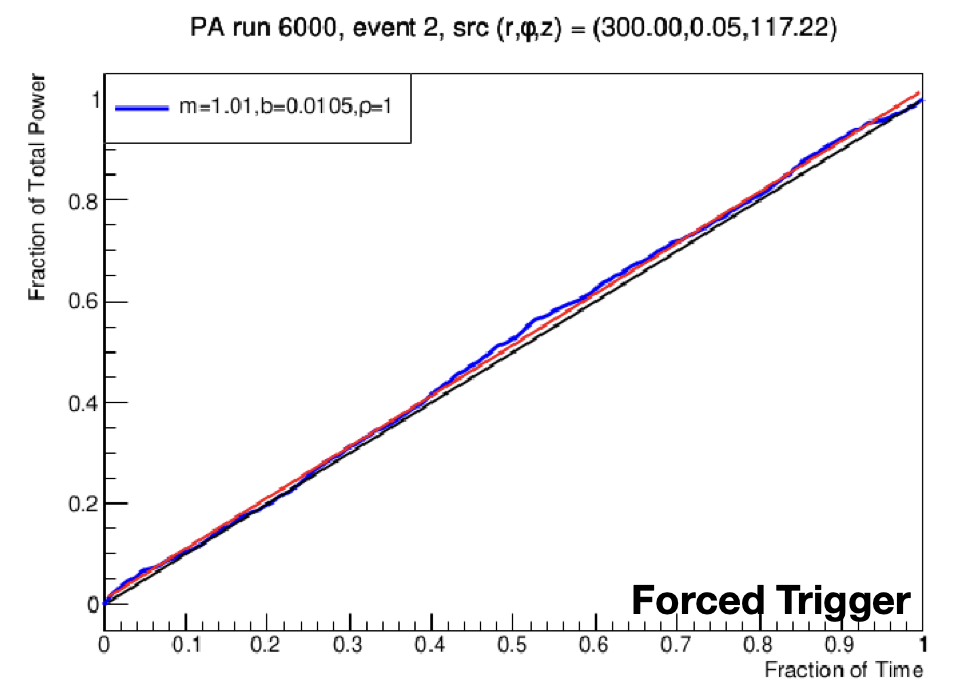
\includegraphics[width=\textwidth]{sections/5sa-analysis/plots/impLin_force_PA.png}
      \end{subfigure}
      ~
      \begin{subfigure}[t]{0.48\textwidth}
        \centering
        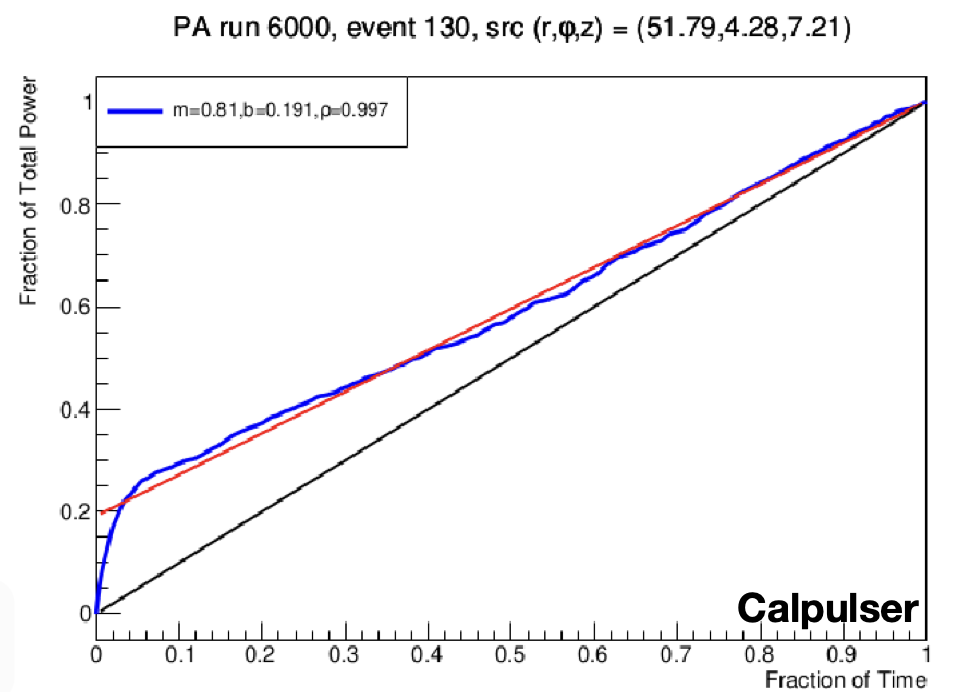
\includegraphics[width=\textwidth]{sections/5sa-analysis/plots/impLin_cp_PA.png}
      \end{subfigure}
      \caption{Example of a linear fit to an event's impulsivity curve courtesy of Marco Muzio.}
      \label{fig:linearimp}
    \end{figure}

    \subsubsection{\texttt{bImp}}

      This variable corresponds to the y-intercept of the linear fit calculated on a waveform's impulsivity CDF.
      Example distributions are shown in Figure~\ref{fig:bImp}.
    
      \begin{figure}
        \centering
        \begin{subfigure}[t]{0.48\textwidth}
          \centering
          \includegraphics[width=\textwidth]{sections/5sa-cleaning/images_variables/a2nu_1d_bImp_v.pdf}
        \end{subfigure}
        ~
        \begin{subfigure}[t]{0.48\textwidth}
          \centering
          \includegraphics[width=\textwidth]{sections/5sa-cleaning/images_variables/a2_10pct_1d_bImp_v.pdf}
        \end{subfigure}
        ~
        \begin{subfigure}[t]{0.48\textwidth}
          \centering
          \includegraphics[width=\textwidth]{sections/5sa-cleaning/images_variables/a2nu_2d_bImp_v_vs_avg_snr_v_rf.pdf}
        \end{subfigure}
        ~
        \begin{subfigure}[t]{0.48\textwidth}
          \centering
          \includegraphics[width=\textwidth]{sections/5sa-cleaning/images_variables/a2nu_2d_bImp_v_vs_global_max_corr_rf.pdf}
        \end{subfigure}
        \caption{
          Top, 1-dimensional distributions of simulated neutrinos following an $E^{-2}$ spectrum (top left) and data (top right) for the analysis variable \texttt{bImp\_v}. 
          The distribution of data has had all cuts applied to RF events except for the final thermal LDA cut described in Section~\ref{sec:lda}.
          The purple curve (which exactly overlays the orange curve) shows these RF events, blue shows software triggered events, and green shows calibration pulser events.
          Bottom, 2-dimensional distributions of simulated neutrinos for the analysis variable \texttt{bImp\_v} as a function of \texttt{avg\_snr\_v} and \texttt{global\_max\_corr\_v}.
        }
        \label{fig:bImp}
      \end{figure}
    
    \subsubsection{\texttt{mImp}}
    
      This variable corresponds to the slope of the linear fit calculated on a waveform's impulsivity CDF.
      Example distributions are shown in Figure~\ref{fig:mImp}.

      \begin{figure}
        \centering
        \begin{subfigure}[t]{0.48\textwidth}
          \centering
          \includegraphics[width=\textwidth]{sections/5sa-cleaning/images_variables/a2nu_1d_mImp_v.pdf}
        \end{subfigure}
        ~
        \begin{subfigure}[t]{0.48\textwidth}
          \centering
          \includegraphics[width=\textwidth]{sections/5sa-cleaning/images_variables/a2_10pct_1d_mImp_v.pdf}
        \end{subfigure}
        ~
        \begin{subfigure}[t]{0.48\textwidth}
          \centering
          \includegraphics[width=\textwidth]{sections/5sa-cleaning/images_variables/a2nu_2d_mImp_v_vs_avg_snr_v_rf.pdf}
        \end{subfigure}
        ~
        \begin{subfigure}[t]{0.48\textwidth}
          \centering
          \includegraphics[width=\textwidth]{sections/5sa-cleaning/images_variables/a2nu_2d_mImp_v_vs_global_max_corr_rf.pdf}
        \end{subfigure}
        \caption{
          Top, 1-dimensional distributions of simulated neutrinos following an $E^{-2}$ spectrum (top left) and data (top right) for the analysis variable \texttt{mImp\_v}. 
          The distribution of data has had all cuts applied to RF events except for the final thermal LDA cut described in Section~\ref{sec:lda}.
          The purple curve (which exactly overlays the orange curve) shows these RF events, blue shows software triggered events, and green shows calibration pulser events.
          Bottom, 2-dimensional distributions of simulated neutrinos for the analysis variable \texttt{mImp\_v} as a function of \texttt{avg\_snr\_v} and \texttt{global\_max\_corr\_v}.
        }
        \label{fig:mImp}
      \end{figure}
    
    \subsubsection{\texttt{rhoImp}}

      This variable corresponds to the correlation coefficient, $\rho$, of the linear fit calculated on a waveform's impulsivity CDF.
      Example distributions are shown in Figure~\ref{fig:rhoImp}.
    
      \begin{figure}
        \centering
        \begin{subfigure}[t]{0.48\textwidth}
          \centering
          \includegraphics[width=\textwidth]{sections/5sa-cleaning/images_variables/a2nu_1d_rhoImp_v.pdf}
        \end{subfigure}
        ~
        \begin{subfigure}[t]{0.48\textwidth}
          \centering
          \includegraphics[width=\textwidth]{sections/5sa-cleaning/images_variables/a2_10pct_1d_rhoImp_v.pdf}
        \end{subfigure}
        ~
        \begin{subfigure}[t]{0.48\textwidth}
          \centering
          \includegraphics[width=\textwidth]{sections/5sa-cleaning/images_variables/a2nu_2d_rhoImp_v_vs_avg_snr_v_rf.pdf}
        \end{subfigure}
        ~
        \begin{subfigure}[t]{0.48\textwidth}
          \centering
          \includegraphics[width=\textwidth]{sections/5sa-cleaning/images_variables/a2nu_2d_rhoImp_v_vs_global_max_corr_rf.pdf}
        \end{subfigure}
        \caption{
          Top, 1-dimensional distributions of simulated neutrinos following an $E^{-2}$ spectrum (top left) and data (top right) for the analysis variable \texttt{rhoImp\_v}. 
          The distribution of data has had all cuts applied to RF events except for the final thermal LDA cut described in Section~\ref{sec:lda}.
          The purple curve (which exactly overlays the orange curve) shows these RF events, blue shows software triggered events, and green shows calibration pulser events.
          Bottom, 2-dimensional distributions of simulated neutrinos for the analysis variable \texttt{rhoImp\_v} as a function of \texttt{avg\_snr\_v} and \texttt{global\_max\_corr\_v}.
        }
        \label{fig:rhoImp}
      \end{figure}

    \subsubsection{\texttt{impLinChi2}}

      This variable corresponds to the $\Chi^2$ calculated for a waveform's impulsivity CDF and its linear fit.
      Example distributions are shown in Figure~\ref{fig:impLinChi2}.
    
      \begin{figure}
        \centering
        \begin{subfigure}[t]{0.48\textwidth}
          \centering
          \includegraphics[width=\textwidth]{sections/5sa-cleaning/images_variables/a2nu_1d_impLinChi2_v.pdf}
        \end{subfigure}
        ~
        \begin{subfigure}[t]{0.48\textwidth}
          \centering
          \includegraphics[width=\textwidth]{sections/5sa-cleaning/images_variables/a2_10pct_1d_impLinChi2_v.pdf}
        \end{subfigure}
        ~
        \begin{subfigure}[t]{0.48\textwidth}
          \centering
          \includegraphics[width=\textwidth]{sections/5sa-cleaning/images_variables/a2nu_2d_impLinChi2_v_vs_avg_snr_v_rf.pdf}
        \end{subfigure}
        ~
        \begin{subfigure}[t]{0.48\textwidth}
          \centering
          \includegraphics[width=\textwidth]{sections/5sa-cleaning/images_variables/a2nu_2d_impLinChi2_v_vs_global_max_corr_rf.pdf}
        \end{subfigure}
        \caption{
          Top, 1-dimensional distributions of simulated neutrinos following an $E^{-2}$ spectrum (top left) and data (top right) for the analysis variable \texttt{impLinChi2\_v}. 
          The distribution of data has had all cuts applied to RF events except for the final thermal LDA cut described in Section~\ref{sec:lda}.
          The purple curve (which exactly overlays the orange curve) shows these RF events, blue shows software triggered events, and green shows calibration pulser events.
          Bottom, 2-dimensional distributions of simulated neutrinos for the analysis variable \texttt{impLinChi2\_v} as a function of \texttt{avg\_snr\_v} and \texttt{global\_max\_corr\_v}.
        }
        \label{fig:impLinChi2}
      \end{figure}


  \pagebreak
  \subsection{Functional Fit Parameters \label{sec:imp_functionalfit}}

    The functional fit uses an equation that roughly describes the Hilbert envelope of a real impulsive signal
    \begin{equation}
      h(t) \propto A e^{- t^2 / B^2 } + 1
      \label{eq:hilbert}
    \end{equation}
    to derive an equation describing the corresponding impulsivity CDF:
    \begin{equation}
      H(\tau) = \frac{ A ~ \text{erf}( \tau / B ) + \tau }{ A ~ \text{erf}( 1 / B ) + 1}
      \label{eq:functionalimp}
    \end{equation}
    where $A$ and $B$ are fit parameters, $\tau$ corresponds to the fraction of time in the waveform, and erf is the error response function. 
    An example of this functional fit applied to real data is shown in Figure~\ref{eq:functionalimp}.

    \begin{figure}[!ht]
      \centering
      \begin{subfigure}[t]{0.48\textwidth}
        \centering
        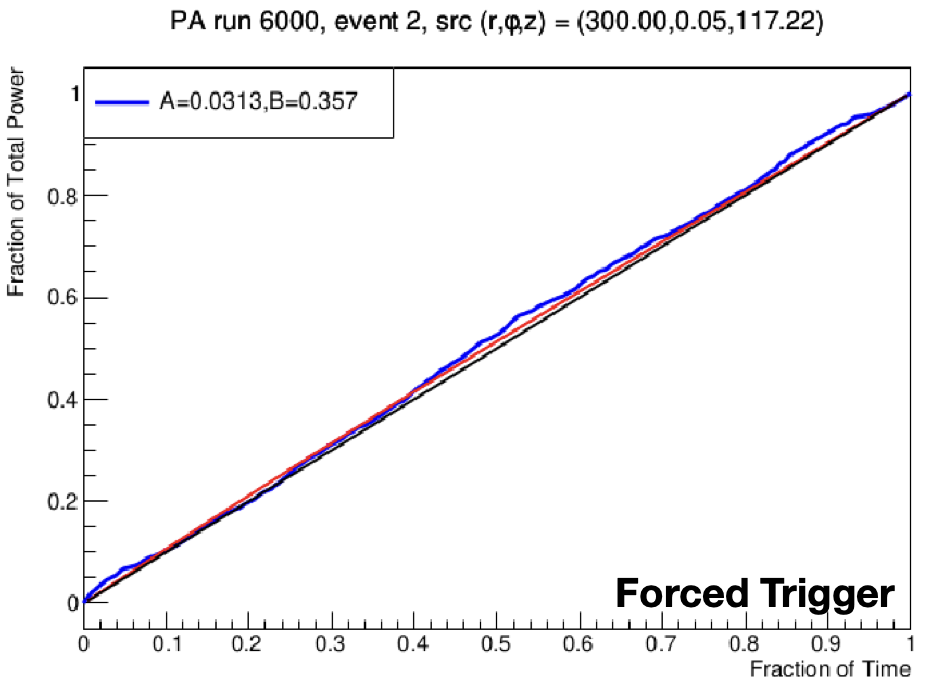
\includegraphics[width=\textwidth]{sections/5sa-analysis/plots/impErf_force_PA.png}
      \end{subfigure}
      ~
      \begin{subfigure}[t]{0.48\textwidth}
        \centering
        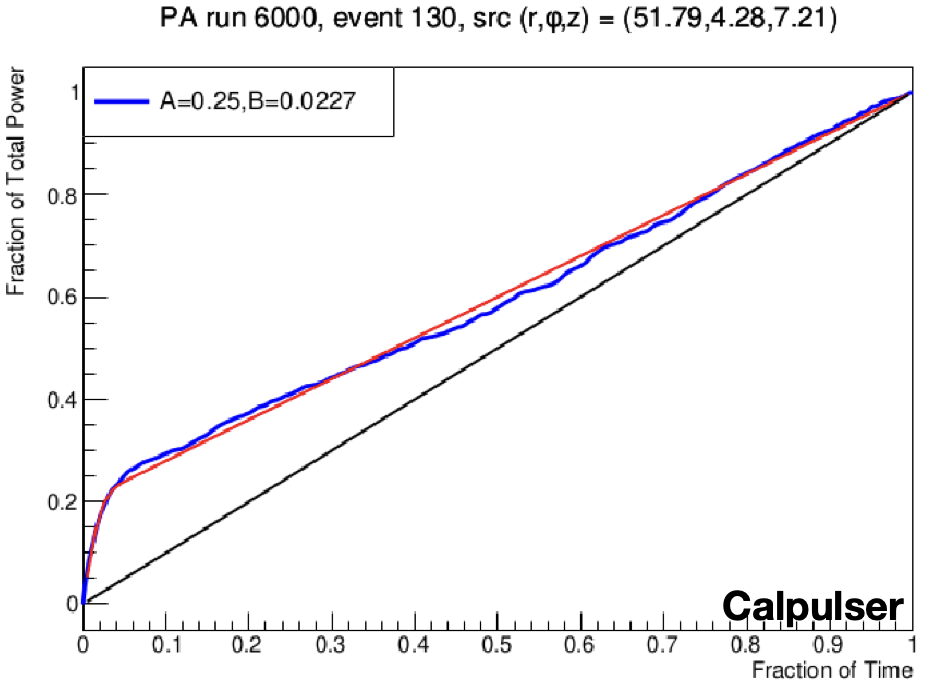
\includegraphics[width=\textwidth]{sections/5sa-analysis/plots/impErf_cp_PA.png}
      \end{subfigure}
      \caption{Example of the hilbert-inspired curve given by Equation~\ref{eq:functionalimp} fit to an event's impulsivity curve.}
      \label{fig:functionalimp}
    \end{figure}
    
    \subsubsection{\texttt{impErfA}}

      This variable corresponds to fit parameter $A$ of the functional impulsivity fit calculated on a waveform's impulsivity CDF, as defined in Equation~\ref{eq:functionalimp}.
      Example distributions are shown in Figure~\ref{fig:impErfA}.
    
      \begin{figure}
        \centering
        \begin{subfigure}[t]{0.48\textwidth}
          \centering
          \includegraphics[width=\textwidth]{sections/5sa-cleaning/images_variables/a2nu_1d_impErfA_v.pdf}
        \end{subfigure}
        ~
        \begin{subfigure}[t]{0.48\textwidth}
          \centering
          \includegraphics[width=\textwidth]{sections/5sa-cleaning/images_variables/a2_10pct_1d_impErfA_v.pdf}
        \end{subfigure}
        ~
        \begin{subfigure}[t]{0.48\textwidth}
          \centering
          \includegraphics[width=\textwidth]{sections/5sa-cleaning/images_variables/a2nu_2d_impErfA_v_vs_avg_snr_v_rf.pdf}
        \end{subfigure}
        ~
        \begin{subfigure}[t]{0.48\textwidth}
          \centering
          \includegraphics[width=\textwidth]{sections/5sa-cleaning/images_variables/a2nu_2d_impErfA_v_vs_global_max_corr_rf.pdf}
        \end{subfigure}
        \caption{
          Top, 1-dimensional distributions of simulated neutrinos following an $E^{-2}$ spectrum (top left) and data (top right) for the analysis variable \texttt{impErfA\_v}. 
          The distribution of data has had all cuts applied to RF events except for the final thermal LDA cut described in Section~\ref{sec:lda}.
          The purple curve (which exactly overlays the orange curve) shows these RF events, blue shows software triggered events, and green shows calibration pulser events.
          Bottom, 2-dimensional distributions of simulated neutrinos for the analysis variable \texttt{impErfA\_v} as a function of \texttt{avg\_snr\_v} and \texttt{global\_max\_corr\_v}.
        }
        \label{fig:impErfA}
      \end{figure}
    
    \subsubsection{\texttt{impErfB}}

      This variable corresponds to fit parameter $B$ of the functional impulsivity fit calculated on a waveform's impulsivity CDF, as defined in Equation~\ref{eq:functionalimp}.
      Example distributions are shown in Figure~\ref{fig:impErfB}.
    
      \begin{figure}
        \centering
        \begin{subfigure}[t]{0.48\textwidth}
          \centering
          \includegraphics[width=\textwidth]{sections/5sa-cleaning/images_variables/a2nu_1d_impErfB_v.pdf}
        \end{subfigure}
        ~
        \begin{subfigure}[t]{0.48\textwidth}
          \centering
          \includegraphics[width=\textwidth]{sections/5sa-cleaning/images_variables/a2_10pct_1d_impErfB_v.pdf}
        \end{subfigure}
        ~
        \begin{subfigure}[t]{0.48\textwidth}
          \centering
          \includegraphics[width=\textwidth]{sections/5sa-cleaning/images_variables/a2nu_2d_impErfB_v_vs_avg_snr_v_rf.pdf}
        \end{subfigure}
        ~
        \begin{subfigure}[t]{0.48\textwidth}
          \centering
          \includegraphics[width=\textwidth]{sections/5sa-cleaning/images_variables/a2nu_2d_impErfB_v_vs_global_max_corr_rf.pdf}
        \end{subfigure}
        \caption{
          Top, 1-dimensional distributions of simulated neutrinos following an $E^{-2}$ spectrum (top left) and data (top right) for the analysis variable \texttt{impErfB\_v}. 
          The distribution of data has had all cuts applied to RF events except for the final thermal LDA cut described in Section~\ref{sec:lda}.
          The purple curve (which exactly overlays the orange curve) shows these RF events, blue shows software triggered events, and green shows calibration pulser events.
          Bottom, 2-dimensional distributions of simulated neutrinos for the analysis variable \texttt{impErfB\_v} as a function of \texttt{avg\_snr\_v} and \texttt{global\_max\_corr\_v}.
        }
        \label{fig:impErfB}
      \end{figure}
    
    \subsubsection{\texttt{impErfLinChi2}}

      This variable corresponds to the $\Chi^2$ calculated for the functional impulsivity fit of a waveform's impulsivity CDF.
      Example distributions are shown in Figure~\ref{fig:impErfLinChi2}.
    
      \begin{figure}
        \centering
        \begin{subfigure}[t]{0.48\textwidth}
          \centering
          \includegraphics[width=\textwidth]{sections/5sa-cleaning/images_variables/a2nu_1d_impErfLinChi2_v.pdf}
        \end{subfigure}
        ~
        \begin{subfigure}[t]{0.48\textwidth}
          \centering
          \includegraphics[width=\textwidth]{sections/5sa-cleaning/images_variables/a2_10pct_1d_impErfLinChi2_v.pdf}
        \end{subfigure}
        ~
        \begin{subfigure}[t]{0.48\textwidth}
          \centering
          \includegraphics[width=\textwidth]{sections/5sa-cleaning/images_variables/a2nu_2d_impErfLinChi2_v_vs_avg_snr_v_rf.pdf}
        \end{subfigure}
        ~
        \begin{subfigure}[t]{0.48\textwidth}
          \centering
          \includegraphics[width=\textwidth]{sections/5sa-cleaning/images_variables/a2nu_2d_impErfLinChi2_v_vs_global_max_corr_rf.pdf}
        \end{subfigure}
        \caption{
          Top, 1-dimensional distributions of simulated neutrinos following an $E^{-2}$ spectrum (top left) and data (top right) for the analysis variable \texttt{impErfLinChi2\_v}. 
          The distribution of data has had all cuts applied to RF events except for the final thermal LDA cut described in Section~\ref{sec:lda}.
          The purple curve (which exactly overlays the orange curve) shows these RF events, blue shows software triggered events, and green shows calibration pulser events.
          Bottom, 2-dimensional distributions of simulated neutrinos for the analysis variable \texttt{impErfLinChi2\_v} as a function of \texttt{avg\_snr\_v} and \texttt{global\_max\_corr\_v}.
        }
        \label{fig:impErfLinChi2}
      \end{figure}
    
  \subsection{\texttt{impSig}}

      This variable calculates the significance of the functional fit (defined in Section~\ref{sec:imp_functionalfit}) compared to the linear fit (defined in Section~\ref{sec:imp_linearfit}).
      Example distributions are shown in Figure~\ref{fig:impSig}.
    
      \begin{figure}
        \centering
        \begin{subfigure}[t]{0.48\textwidth}
          \centering
          \includegraphics[width=\textwidth]{sections/5sa-cleaning/images_variables/a2nu_1d_impSig_v.pdf}
        \end{subfigure}
        ~
        \begin{subfigure}[t]{0.48\textwidth}
          \centering
          \includegraphics[width=\textwidth]{sections/5sa-cleaning/images_variables/a2_10pct_1d_impSig_v.pdf}
        \end{subfigure}
        ~
        \begin{subfigure}[t]{0.48\textwidth}
          \centering
          \includegraphics[width=\textwidth]{sections/5sa-cleaning/images_variables/a2nu_2d_impSig_v_vs_avg_snr_v_rf.pdf}
        \end{subfigure}
        ~
        \begin{subfigure}[t]{0.48\textwidth}
          \centering
          \includegraphics[width=\textwidth]{sections/5sa-cleaning/images_variables/a2nu_2d_impSig_v_vs_global_max_corr_rf.pdf}
        \end{subfigure}
        \caption{
          Top, 1-dimensional distributions of simulated neutrinos following an $E^{-2}$ spectrum (top left) and data (top right) for the analysis variable \texttt{impSig\_v}. 
          The distribution of data has had all cuts applied to RF events except for the final thermal LDA cut described in Section~\ref{sec:lda}.
          The purple curve (which exactly overlays the orange curve) shows these RF events, blue shows software triggered events, and green shows calibration pulser events.
          Bottom, 2-dimensional distributions of simulated neutrinos for the analysis variable \texttt{impSig\_v} as a function of \texttt{avg\_snr\_v} and \texttt{global\_max\_corr\_v}.
        }
        \label{fig:impSig}
      \end{figure}

  % https://aradocs.wipac.wisc.edu/cgi-bin/DocDB/ShowDocument?docid=2964 impulsivity metrics
  
\pagebreak
\section{\texttt{mindepth\_v} \label{sec:mindepth}}

  \begin{figure}[!ht]
    \centering
    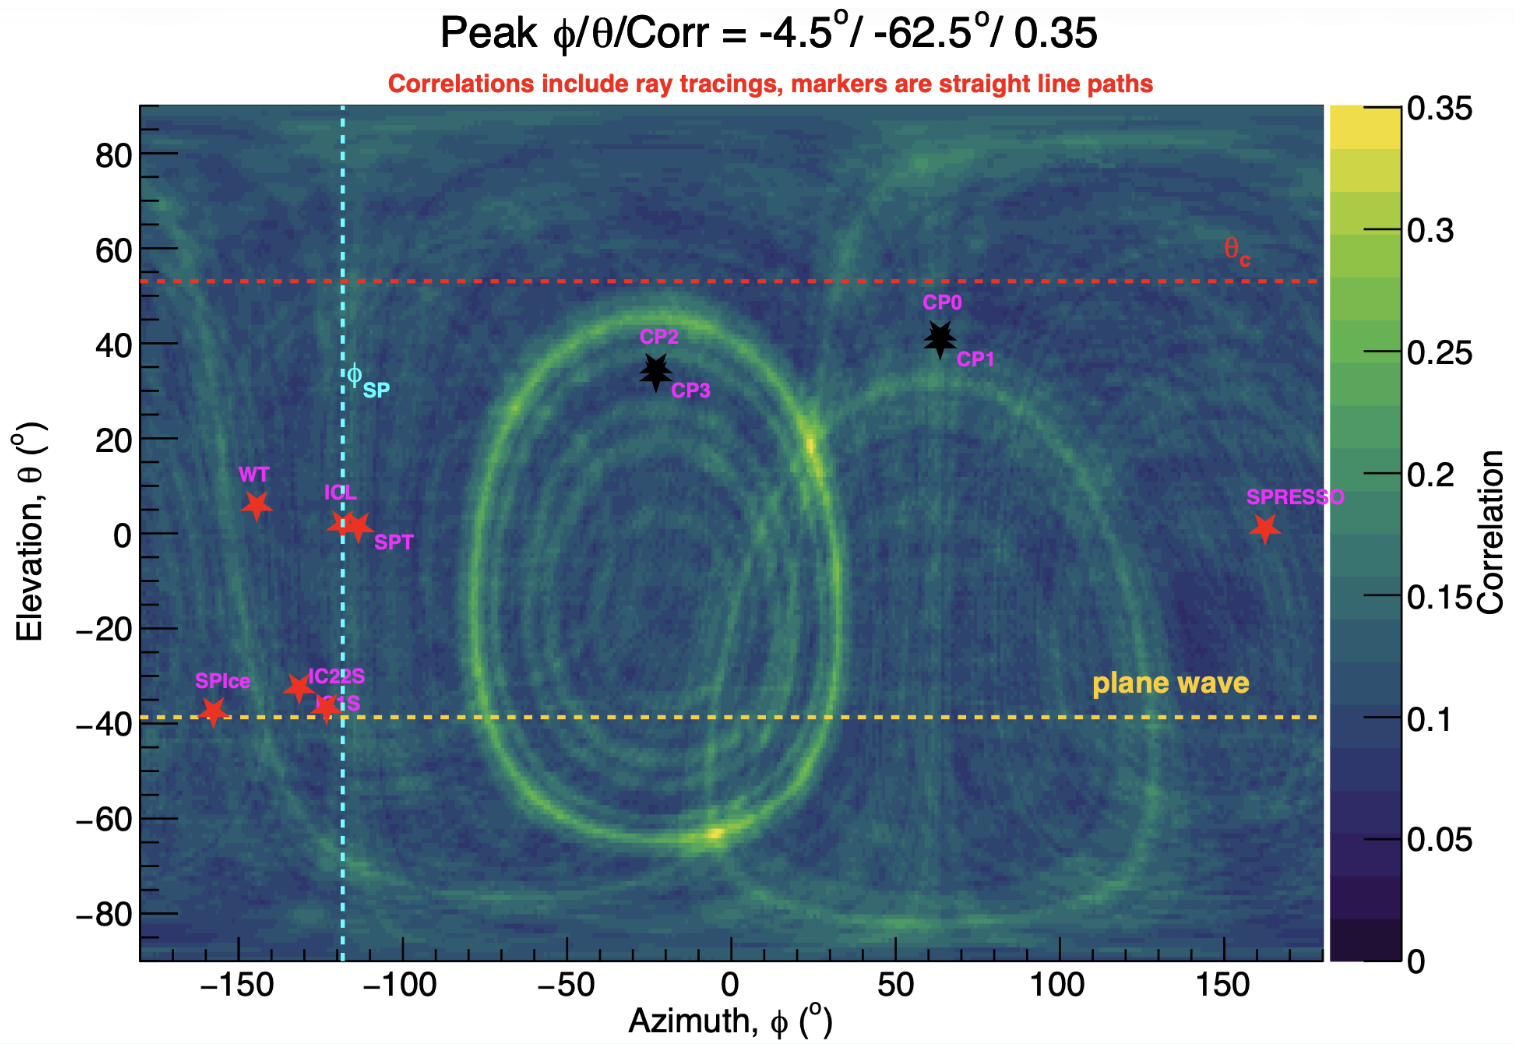
\includegraphics[
        width=0.75\textwidth,
        alt={}
    ]{sections/5sa-cleaning/images/a1r3183e65990_mindepth.pdf}
    \caption{An example of an event with a high \texttt{mindepth\_v}, meaning this event has many possible reconstructions that imply this event originated near the surface. This example is A1, run 3183, event 65990.}
    \label{fig:lowmindepth}
  \end{figure}

  This variable is calculated using the map of correlation values for all locations on the sky in azimuth and elevation to identify the highest elevation in the reconstruction map with a correlation value $\geq 60$\% of the map's maximimum correlation value.
  Taking Figure~\ref{fig:lowmindepth} for example, the maximum correlation value of this reconstruction skymap is 0.35 and we find the highest elevation a location on the sky with a correlation score of 0.21 ($0.6 \times 3.5$) is at an elevation of 68.5$^{\circ}$.
  We take this one step further and convert this maximum elevation angle into a minimum depth from the surface 
  \begin{equation}
    d = z_{\text{SC}} - r \sin{\theta}
    \label{eq:mindepth}
  \end{equation}
  where $z_{\text{SC}}$ is the average antenna depth for the station, $r$ is the radius of the reconstruction sphere, and $\theta$ is the elevation angle.
  For Figure~\ref{fig:lowmindepth}, which is the reconstruction of an A1 event using the pulser map radius (defined in Tab.~\ref{tab:cpdist}), $z_{\text{SC}}=-67.5$~m and $r=48.02$~m.
  This yields a \texttt{mindepth\_v}$=22.7$~m for this event. 
  This conversion to \texttt{mindepth\_v} was done to more easily compare our event reconstructions to the average depth of cosmic ray cores that impact into the ice - the deepest surface-related background we expect to observe, in theory.
  Example distributions are shown in Figure~\ref{fig:mindepthv}.
    
  \begin{figure}
    \centering
    \begin{subfigure}[t]{0.48\textwidth}
      \centering
      \includegraphics[width=\textwidth]{sections/5sa-cleaning/images_variables/a2nu_1d_mindepth_v.pdf}
    \end{subfigure}
    ~
    \begin{subfigure}[t]{0.48\textwidth}
      \centering
      \includegraphics[width=\textwidth]{sections/5sa-cleaning/images_variables/a2_10pct_1d_mindepth_v.pdf}
    \end{subfigure}
    ~
    \begin{subfigure}[t]{0.48\textwidth}
      \centering
      \includegraphics[width=\textwidth]{sections/5sa-cleaning/images_variables/a2nu_2d_mindepth_v_vs_avg_snr_v_rf.pdf}
    \end{subfigure}
    ~
    \begin{subfigure}[t]{0.48\textwidth}
      \centering
      \includegraphics[width=\textwidth]{sections/5sa-cleaning/images_variables/a2nu_2d_mindepth_v_vs_global_max_corr_rf.pdf}
    \end{subfigure}
    \caption{
      Top, 1-dimensional distributions of simulated neutrinos following an $E^{-2}$ spectrum (top left) and data (top right) for the analysis variable \texttt{mindepth\_v}. 
      The distribution of data has had all cuts applied to RF events except for the final thermal LDA cut described in Section~\ref{sec:lda}.
      The purple curve (which exactly overlays the orange curve) shows these RF events, blue shows software triggered events, and green shows calibration pulser events.
      Bottom, 2-dimensional distributions of simulated neutrinos for the analysis variable \texttt{mindepth\_v} as a function of \texttt{avg\_snr\_v} and \texttt{global\_max\_corr\_v}.
    }
    \label{fig:mindepthv}
  \end{figure}


\pagebreak
\section{\texttt{wavefront\_rms\_v}}

  \texttt{wavefront\_rms} is a measure of how compatible observed waveforms are with an arriving plane wave. 
  We use a simplified version of what was originally proposed by Carl Pfender and explained in~\citep{thesis_clark}
  For like-polarization antennas, we determine the time of maximum peak-to-peak (maximum-to-minimum) voltage in any 20 nanosecond window over the whole waveform.
  We then assume, for the purpose of this calculation, that the signal from a potential plane wave arrived at this antenna at this time of maximum peak-to-peak voltage separation.
  For each pair of antennas, the time difference between these maximum peak-to-peak times is used to calculate the arrival angle of the signal as
  \begin{equation}
    cos(\theta) = \frac{c \Delta t}{n \Delta d}
    \label{eq:wavefrontrms}
  \end{equation}
  where $c$ is the speed of light in a vacuum, $\Delta t$ is the time delay between antennas, $n$ is the refractive index of the medium (ice), and $\Delta d$ is the distance between the two antennas. 
  When comparing the arrival angle calculated by each pair of antennas, if a plane wave was observed then these arrival angles should all be similar. 
  If a thermal-like event was observed, then these calculated arrival angles should all be quite different from each other. 
  To quantify this, we calculate the variance of all the calculated arrival angles (contrary to the variable name of ``RMS'').
  When this variance, the \texttt{wavefront\_rms}, is small, the recorded waveform has a strong likelihood of originating from a plane wave and when it is large, this scenario is less likely.
  Example distributions are shown in Figure~\ref{fig:wavefront_rms}.
    
  \begin{figure}
    \centering
    \begin{subfigure}[t]{0.48\textwidth}
      \centering
      \includegraphics[width=\textwidth]{sections/5sa-cleaning/images_variables/a2nu_1d_wavefront_rms_v.pdf}
    \end{subfigure}
    ~
    \begin{subfigure}[t]{0.48\textwidth}
      \centering
      \includegraphics[width=\textwidth]{sections/5sa-cleaning/images_variables/a2_10pct_1d_wavefront_rms_v.pdf}
    \end{subfigure}
    ~
    \begin{subfigure}[t]{0.48\textwidth}
      \centering
      \includegraphics[width=\textwidth]{sections/5sa-cleaning/images_variables/a2nu_2d_wavefront_rms_v_vs_avg_snr_v_rf.pdf}
    \end{subfigure}
    ~
    \begin{subfigure}[t]{0.48\textwidth}
      \centering
      \includegraphics[width=\textwidth]{sections/5sa-cleaning/images_variables/a2nu_2d_wavefront_rms_v_vs_global_max_corr_rf.pdf}
    \end{subfigure}
    \caption{
      Top, 1-dimensional distributions of simulated neutrinos following an $E^{-2}$ spectrum (top left) and data (top right) for the analysis variable \texttt{wavefront\_rms\_v}. 
      The distribution of data has had all cuts applied to RF events except for the final thermal LDA cut described in Section~\ref{sec:lda}.
      The purple curve (which exactly overlays the orange curve) shows these RF events, blue shows software triggered events, and green shows calibration pulser events.
      Bottom, 2-dimensional distributions of simulated neutrinos for the analysis variable \texttt{wavefront\_rms\_v} as a function of \texttt{avg\_snr\_v} and \texttt{global\_max\_corr\_v}.
    }
    \label{fig:wavefront_rms}
  \end{figure}


  \end{appendices}

%% Are you a big nerd with a colophon?  Add it here.
\singlespacing
\begin{colophon}
\input{backmatter/colophon}
\end{colophon}

%% McBride is a very nice style (some version is included in this distribution)
\bibliographystyle{aasjournal}
\bibliography{bibliography}

%% Want an index?  Neither did I.
\printindex

\end{document}
